%!TEX TS-program = xelatex
%---------------------------------------------------------------------------%
%->> 深圳大学毕业论文模板
%---------------------------------------------------------------------------%
%- 载入模板类
\documentclass{szuthesis}% 默认形式
% \documentclass[print]{szuthesis}% 打印预览版本,可以自动生成额外的空白页用于打印
% \documentclass[fontset=windows|adobe|mac|ubuntu]{szuthesis}% 选择字库
%---------------------------------------------------------------------------%
% - 载入配置信息,包含论文封面信息、必要的package
%---------------------------------------------------------------------------%TITLE
%->> Cover information 封面信息
%---------------------------------------------------------------------------%
\classid{\ TP39\;}% 分类号
\udc{\ \ \ 004\ \ }
\confidential{\ \ \ \ \ 公开}% 密级
%- 注:\title包含两个参数
% \title{深圳大学\LaTeX{}模板}{}% 单行题目,第二个参数为空
\title{***}{}% 多行题目
%- 注:英文题目用于生成Abstract的页眉,只有一个参数
\TITLE{***}
\author{\ \ \ \ \ \ \ \ ***}% 论文作者
\idnumber{\ \ \ \ \ \ \ \ ***}
\major{\ \ \ \ \ \ \ \ 计算机科学与技术}% 学科专业名称
\dtype{\ \ \ \ \ \ \ \ 工学}
%- 注:以下两个类型支持多行
\institute{\ \ \ \ \ \ \ \ 计算机与软件学院}% 院系名称单行
% \institute{某某学院\\某某实验室}% 院系名称多行
\advisor{\ \ \ \ \ \ \ \ ***}% 指导教师单行v
% \advisor{张老师\ 教授\\王老师\ 研究员}% 指导教师多行
\DEGREE{MasterXS}% 学术硕士
% \DEGREE{MasterZY}\degree{\ \ \ \ \ \ \ \ \ \ \ \ \ \ \ \ 工程硕士}% 专业硕士
%---------------------------------------------------------------------------%
%->> other config
%---------------------------------------------------------------------------%
%- 添加两个命令方便输出
\DeclareRobustCommand\cs[1]{\texttt{\char`\\#1}}
\providecommand\pkg[1]{{\sffamily#1}}
%-
\addbibresource{Biblio/ref.bib}% 参考文献路径
\setlength\bibitemsep{0.0ex plus 0.2ex minus 0.2ex}% set distance between bib entrie
%-
\setcounter{tocdepth}{3}% depth for the table of contents,设为2可不显示subsubsection
\setcounter{secnumdepth}{3}% depth for section numbering, default is 2
%-
%- 某些小语种会超出版面边界,提示Overfull \hbox{}...,中英日韩无需使用(或使用宏包microtype)
% \setlength\emergencystretch{1em}
%-
%- 重新设置 equation, figure, table 的序号
%\numberwithin{equation}{section}% set enumeration level
%\renewcommand{\theequation}{\thesection\arabic{equation}}% configure the label style
%\numberwithin{figure}{section}% set enumeration level
%\renewcommand{\thefigure}{\thesection\arabic{figure}}% configure the label style
%\numberwithin{table}{section}% set enumeration level
%\renewcommand{\thetable}{\thesection\arabic{table}}% configure the label style
\counterwithout{footnote}{chapter}% footnote编号全局连续
%-
%---------------------------------------------------------------------------%
%->> Package
%---------------------------------------------------------------------------%
% -> szuthesis.cls中已经导入的包
% - etoolbox, a toolbox of programming facilities
% - geometry, for layout
% - expl3, LaTeX3 programming environment
% - array
% - ulem, underline
% - xeCJKfntef, underline for CJK
% - fancyhdr, header and footer
% - biblatex
%-
\usepackage{titlesec}
\usepackage{ctex}
\xeCJKsetup{AutoFakeBold=true}
\usepackage{multirow}
\usepackage{hyperref}
\usepackage{makecell}
\usepackage{graphicx}
\usepackage{adjustbox}
\DeclareGraphicsExtensions{.pdf,.jpg,.png,.eps,.tif,.bmp}% 默认图片格式
\graphicspath{{Image/}}% 默认图片检索路径
%-
% \usepackage[format=plain,hangindent=2.0em,font={small},skip=8pt,labelsep=space,labelfont={bf,\song},textfont={bf,\song}]{caption}
\usepackage{fontspec}
\usepackage[format=plain,hangindent=2.0em,skip=8pt,labelsep=space]{caption}
\DeclareCaptionFont{songsong}{\song}
\captionsetup{
    font={small,bf,songsong}
}
%-
% \captionsetup{
%     figurename=图,
%     tablename=表,
%     labelsep=space, % 标签和文本之间的分隔符为一个空格
%     labelfont=bf, % 标签字体加粗
%     textfont=bf % 文本字体加粗
% }

\renewcommand{\thefigure}{\thechapter-\arabic{figure}} % 重新定义图的编号格式
\renewcommand{\thetable}{\thechapter-\arabic{table}} % 重新定义表的编号格式

\renewcommand{\theequation}{\thechapter-\arabic{equation}} % 重新定义公式的编号格式
% \captionsetup{font={\song\zihao{5}}}
\usepackage{subcaption}% 处理子图
%-
% \usepackage[list=off]{bicaption} % 双语caption
% \DeclareCaptionOption{bi-second}[]{
%     \def\tablename{Table}%
%     \def\figurename{Figure}%
% }
% \captionsetup[bi-second]{bi-second}
%-
\usepackage[section]{placeins}% 阻止图片浮动超出当前section
%-
\usepackage{enumitem}% 列表环境功能提升
\setlist{nosep}% 默认文本行间距
% \setlist[enumerate]{wide=\parindent}% 是否悬挂对齐,不建议全局修改
% \setlist[itemize]{wide=\parindent}
%-
% \usepackage{verbatim}
%-
% \usepackage{chemfig}% draw 2D chemical structures
% \usepackage[version=4]{mhchem}% typeset chemical formulae [mhchem|chemformula]
%-
% \usepackage{microtype}% improves general appearance of the text, 启用后降低编译效率
%-
% \usepackage{pdflscape}% landscape environment, \begin{landscape} ... \end{landscape}
%-
% \usepackage[usenames,dvipsnames,svgnames,table]{xcolor}% color support
%-
% \usepackage{tikz}% automatically load pgf package, plot with tex
% \usetikzlibrary{positioning, arrows, calc, trees }%
%-
\usepackage{booktabs} % 三线表
\usepackage{siunitx} % Required for S column type
% \usepackage{multirow} % For multirow feature
\usepackage{array}    % For table column formatting
\usepackage{rotating} % For \rotatebox
% \usepackage{graphicx}
\usepackage{amssymb} % For checkmark and xmark
%-
% \usepackage{tikz}
\usepackage{import}

\usetikzlibrary{3d}
\usepackage{pgfplots}
\pgfplotsset{compat=1.17}
\usepackage{xcolor}


% %%%%%%%%%%%%%%%%%%%%%%%%%%%%%%%%%%%%%%%%%%%%%%%%%%%%%%%%%%%%%%%%%%%%%%%%%%%%%%%%%%%%%%%%%%%%%%%%%%%%%%%%%%%%%%%%%%%%%%%%%%%%%%%%%%%
% %%%%%%%%%%%%%%%%%%%%%%%%%%%%%%%%%%%%%%%%%%%%%%%%%%%%%%%%%%%%%%%%%%%%%%%%%%%%%%%%%%%%%%%%%%%%%%%%%%%%%%%%%%%%%%%%%%%%%%%%%%%%%%%%%%%
% % \documentclass[border=8pt, multi, tikz]{standalone} 

% \subimport{./layers/}{init}
% \usetikzlibrary{positioning}
% \usetikzlibrary{3d} %for including external image 

% \def\ConvColor{rgb:yellow,5;red,2.5;white,5}
% \def\ConvReluColor{rgb:yellow,5;red,5;white,5}
% \def\PoolColor{rgb:red,1;black,0.3}
% \def\UnpoolColor{rgb:blue,2;green,1;black,0.3}
% \def\FcColor{rgb:blue,5;red,2.5;white,5}
% \def\FcReluColor{rgb:blue,5;red,5;white,4}
% \def\SoftmaxColor{rgb:magenta,5;black,7}   
% \def\SumColor{rgb:blue,5;green,15}
% \def\ConcatColor{rgb:blue,5;red,2.5;white,5}
% \definecolor{TimeEmbedColor}{RGB}{88,88,88}

% \newcommand{\copymidarrow}{\tikz \draw[-Stealth,line width=0.8mm,draw={rgb:blue,4;red,1;green,1;black,3}] (-0.3,0) -- ++(0.3,0);}
% %%%%%%%%%%%%%%%%%%%%%%%%%%%%%%%%%%%%%%%%%%%%%%%%%%%%%%%%%%%%%%%%%%%%%%%%%%%%%%%%%%%%%%%%%%%%%%%%%%%%%%%%%%%%%%%%%%%%%%%%%%%%%%%%%%%
% %%%%%%%%%%%%%%%%%%%%%%%%%%%%%%%%%%%%%%%%%%%%%%%%%%%%%%%%%%%%%%%%%%%%%%%%%%%%%%%%%%%%%%%%%%%%%%%%%%%%%%%%%%%%%%%%%%%%%%%%%%%%%%%%%%%

% \usetikzlibrary{quotes,arrows.meta}
% \usetikzlibrary{positioning}
% \def\edgecolor{rgb:blue,4;red,1;green,4;black,3}
% \newcommand{\midarrow}{\tikz \draw[-Stealth,line width =0.8mm,draw=\edgecolor] (-0.3,0) -- ++(0.3,0);}

% \usepackage{}
% \usepackage{Box}
% \usepackage{RightBandedBox}

\usepackage{listings}% 代码片段
\def\lstlistingname{代码}
\lstset{%
    basicstyle=\linespread{1.2}\small, % 字体
    breaklines=true,                   % 自动换行
    frame=lines,                       % 上下的边框,可选none|single|shadowbox等
    keepspaces=true,
    showstringspaces=false,            % string的空格添加标记,defaul:true
    tabsize=2,                         % tab长度
    % stringstyle=\color{DarkViolet},
    % backgroundcolor=\color{gray!10},
    % commentstyle=\color{ForestGreen},
    % keywordstyle=\color{blue},
}
%-
% \usepackage{amsmath,amsfonts}
% \usepackage{bm}
% \usepackage{array}
% \usepackage{booktabs}
% \usepackage{longtable}
\usepackage{tabularx}
% \usepackage{algorithm}
% \usepackage{algorithmic}
\usepackage{diagbox}
% \usepackage[boxed,ruled,lined]{algorithm2e}
\usepackage[ruled,vlined,linesnumbered]{algorithm2e} % 算法描述
\SetAlgorithmName{算法}{}{}
\SetArgSty{textit}
% 设置算法标题的字体样式
\SetAlCapNameFnt{\zihao{5}\song}
\SetAlCapFnt{\zihao{5}\song}
\SetAlgoCaptionSeparator{:}
% 设置算法体的整体字体
\SetAlFnt{\zihao{5}\song\itshape}
\renewcommand{\thealgocf}{\thechapter-\arabic{algocf}}%重新定义算法编号

%重置算法计数器
\makeatletter
\@addtoreset{algocf}{chapter}
\makeatother
%---------------------------------------------------------------------------%
%->> 配置数学环境
%---------------------------------------------------------------------------%

\usepackage{pifont}
\newcommand*{\dif}{\mathop{}\!\mathrm{d}}
%- 符号表,参考 http://milde.users.sourceforge.net/LUCR/Math/mathpackages/amssymb-symbols.pdf
\usepackage{amsthm} % 定理引理等环境
\theoremstyle{plain}% for theorems, lemmas, propositions, etc
\newtheorem{theorem}              {定理} [chapter]
\newtheorem{axiom}      [theorem] {公理}
\newtheorem{lemma}      [theorem] {引理}
\newtheorem{corollary}  [theorem] {推论}
\newtheorem{assertion}  [theorem] {断言}
\newtheorem{proposition}[theorem] {命题}
\newtheorem{conjecture} [theorem] {猜想}
\newtheorem{assumption} [theorem] {假设}
\theoremstyle{definition}% for definitions and examples
\newtheorem{definition}           {定义} [chapter]
\newtheorem{example}              {例}   [chapter]
\newtheorem{problem}              {问题} [chapter]
\newtheorem{exercise}             {练习} [chapter]
\theoremstyle{remark}% for remarks and notes
\newtheorem*{remark}              {注}
\newtheorem*{solution}            {解}
% \usepackage{mathtools}
\usepackage{unicode-math}
%- 注:unicode-math可以配置数学公式字体,注意包冲突!
%- 已知可能存在冲突的包:amscd,amsfonts,bbm,bm,eucal,eufrak,mathrsfs
\setmathfont{XITSMath-Regular}[
    Extension=.otf, BoldFont=XITSMath-Bold, Ligatures=TeX, StylisticSet = 1,
]
\setmathfont{XITSMath-Regular}[
    Extension=.otf, range={scr,bfscr}, Ligatures=TeX, StylisticSet = 2,
]
\setmathfont{XITSMath-Regular}[
    Extension=.otf, range={cal,bfcal}, Ligatures=TeX, StylisticSet = 1,
]
% \setmathfont{XITS Math Bold}[version=bold]% for bold version % 不兼容StylisticSet=2
% \newenvironment{szumathbf}{\bfseries\mathversion{bold}}{}
\def\XITSMathFontOptions{
    Extension=.otf, BoldFont=XITSMath-Bold, Ligatures=TeX, StylisticSet = 1
}
\setmathrm{XITSMath-Regular}[\XITSMathFontOptions]
\setmathsf{XITSMath-Regular}[\XITSMathFontOptions]
\setmathtt{XITSMath-Regular}[\XITSMathFontOptions]
%-
\def\boldsymbol#1{\symbfit{#1}}
\providecommand{\Vector}[1]{\symbfit{#1}}
\providecommand{\Matrix}[1]{\symbfit{#1}}
\providecommand{\Tensor}[1]{\symbfit{#1}}
\providecommand{\Dif}{\symrm{d}}
\providecommand{\Const}[1]{\symrm{#1}}
\providecommand{\deltarm}{\symrm{\delta}}
\providecommand{\Div}{\operatorname{div}}
\providecommand{\Trace}{\operatorname{tr}}
%---------------------------------------------------------------------------%
%->> 链接,生成书签,在最后
%---------------------------------------------------------------------------%
\usepackage{hyperref}% 超链接,生成书签,[注:放在最后]
\hypersetup{% set hyperlinks
    pdfencoding=auto,% allows non-Latin based languages in bookmarks
    psdextra=true,% extra support for math symbols in bookmarks
    bookmarksnumbered=true,% put section numbers in bookmarks
    pdftitle={\szutitle},% title
    pdfauthor={\szuauthor},% author
    pdfsubject={\szutitle},% subject
    pdfstartview={FitH},% fits the width of the page to the window
    % colorlinks=true,% false: boxed links; true: colored links
    % linkcolor=black,% color of internal links
    % citecolor=blue,% color of links to bibliography
    % filecolor=blue,% color of file links
    % urlcolor=blue,% color of external links
    hidelinks,% hide links color and box
}
%---------------------------------------------------------------------------%
%->> END
%---------------------------------------------------------------------------%

%---------------------------------------------------------------------------%
%- 辅助命令,后文中的所有\include均可在此单独列出,用逗号隔开,
%- 以此只编译必要的章节,加快编译速度,待全文完成后可注释本命令,即可编译全文。
%- 也可注释部分内容,正文中所有的内容均可注释后避免其参与编译,包含maketitle等命令,
%- 执行此命令或注释后可能导致章节序号发生错误,无需担心,全文编译后即可恢复
% \includeonly{Tex/Abstract,Tex/Appendix}
% %---------------------------------------------------------------------------%
\begin{document}
%-
\maketitle% 制作封面
%-
%- 声明包含两种形式,
%- 如果参数为空则可自动生成默认声明页,也可设置参数导入签字后的扫描版PDF文件
% \makedeclaration{declaration}% 制作声明,参数为扫描版文件名,默认在Image下
\makedeclaration{}% 制作声明,自动生成
%-
\frontmatter% 初始化摘要页环境,不建议注释
%-
%---------------------------------------------------------------------------%
%->> Abstract
%---------------------------------------------------------------------------%
%-
%-> 中文摘要
%-
\begin{abstract}
    \markboth{摘\quad 要}{}
中文摘要
    
\keywords{短文本,主题模型,数据增强,变分自编码器,数据挖掘}% 中文关键词
\end{abstract}
%-
%-> 英文摘要
%-
\begin{ABSTRACT}
ABSTRACT


\KEYWORDS{short text, topic model, data augmentation, variational autoencoder, data mining}% 英文关键词
\end{ABSTRACT}
%---------------------------------------------------------------------------%
%-
\tableofcontents% 目录
%-
\mainmatter% 初始化正文环境,不建议注释
%-
\chapter{绪论}\label{chap:intro}

\section{研究背景}\label{sec:background}
随着信息技术和互联网媒体的崛起,如博客、维基百科、社交媒体平台等,文本数据已经成为当代社会信息传播的重要载体。其中,短文本作为信息传播的一种高效形式,其数量在互联网时代经历了爆炸性的增长。短文本通常指的是字数较少、内容简洁的文本数据。它们的主要特点是信息量密集,但表达形式极为简洁。比如在社交平台中,不论是用户发表的微博和小红书,还是标题、弹幕以及评论等,绝大多数都以短文本的形式存在。由于短文本在个人日常交流、商业广告、新闻报道等领域扮演着重要的角色,对短文本进行分析研究不仅对于理解和挖掘网络社会的信息动态具有重要意义,也对于商业智能和公共管理等领域的决策支持具有实际价值。

目前,主题模型仍是一种高效挖掘短文本数据集的常用算法。主题挖掘能够自动发现文本中隐藏的主题,是为了文本信息提取这一任务所设计的一类无监督机器学习技术,使得人们能够更快速且全面地理解文本所包含的内容。该方法通过对文档语料库进行统计分析,能够将包含大量文档的语料库压缩成一个简短的摘要,以揭示语料库中的潜在主题。这个简短的摘要采用主题的形式,即一组相关的词语,因此被称为主题模型。同时,每个文档可以被表示为在这些潜在主题上的一个分布。这种“文档-主题-词”结构提供了语义可解释性,使我们能够更好地理解语料库所包含的主题信息。

基于主题模型的有效性和可解释性,短文本主题挖掘在现实生活中得到了广泛的应用。例如,在商业领域,通过分析消费者的短评和反馈,能够及时捕捉市场趋势和消费者需求,为产品开发和市场营销提供指导。在社交媒体分析中,通过对大量用户发表的短文本进行主题挖掘,可以迅速了解公众情绪、舆论走向或热点话题。自动检测社交媒体上的事件讨论,这在许多不同的领域中都有用途。例如,在国家安全行动中用于预测骚乱并检测虚假信息\cite{DisruptiveEventDetection},而人为地监控社交媒体中的反社会行为和反事实行为是十分受限制的。利用主题模型,可以深入挖掘和利用海量短文本背后有价值的信息。
    
%由于主题模型的有效性和可解释性,主题挖掘在现实生活中得到了广泛的应用。举例来说,在医疗领域,电子健康记录提供了丰富的临床信息,使用主题模型可以提取流行病学模式以了解和预测患者的疾病风险\cite{PredictDisease}。另一个例子是自动检测社交媒体上的事件讨论,这在许多不同的领域中都有用途。例如,在国家安全行动中用于预测骚乱并检测虚假信息\cite{DisruptiveEventDetection},而人为地监控社交媒体中的反社会行为和反事实行为是十分受限制的。此外,社交网络舆情已成为风险防范管理的重要情报源,从中检测及分析事件将成为实时了解业务风险和廉政风险动态,进而及时开展风险布控和纪检监察行动的重要渠道之一。
\subsection{短文本特征概述}
随着社交媒体和电商平台的不断发展,短文本已经成为当今互联网时代常见的一类文本。短文本的长度,少则几个词,多则十几个词,与常规长度的文本相比存在相当大的差别。传统的书籍和科学文章存在着具有辨识度的单词共现模式,而短文本可能拥有非常不同的模式\cite{survey_2023}。短文本数据,尤其是互联网中的短文本,具有如下的特征:(1)稀疏性:社交媒体短文本不同于编辑精良的文章,往往只包含少数匆忙输入的单词。因此短文本的长度十分有限。此外,社交媒体数据的词汇不断演变,新词和标签不断涌现。帖子中包含多种语言并不罕见,缩写更是常规。在社交媒体帖子中,相较于长文本,高频的单词共现模式几乎不存在。(2)语境缺失:由于篇幅限制,短文本往往缺乏足够的上下文信息来清晰地表达其含义。这使得理解和分析短文本的语义内容更加困难。(3)动态性和时效性:社交媒体等平台上的短文本往往与当前事件、趋势和公众关注点密切相关,展现出强烈的动态性和时效性。(4)潜在主题的复杂性:单个短文本所包含的信息有限,但文本与文本之间的联系可以揭示复杂且多样的主题信息。
% \subsection{短文本特征概述}
% 随着社交媒体和电商平台的不断发展,短文本已经成为当今互联网时代常见的一类文本。比如在社交平台中,不论是用户发表的微博和小红书,还是标题、弹幕以及评论等,绝大多数都是短文本。这些文本的长度,少则几个词,多则十几个词,和常规长度的文本相比存在相当大的差别。与常规文本不同,短文本数据,尤其是互联网中的短文本,具有如下的特征\cite{Evolution}:
%此外,传统的主题模型主要聚焦于常规文本的主题挖掘,如NMF\cite{NMF}(Non-negative Matrix Factorization)和LDA\cite{LDA}(Latent Dirichlet Allocation)等在发现学术文章等长文本的潜在主题结构上有着强大的能力\cite{StrongAbility}。这促使我们希望在短文本上实现类似的强大和准确的效果。然而,在对社交媒体等短文本语料进行分析时,传统主题模型的表现并不理想。

% \begin{itemize}
%     \item[(1)] 稀疏性。社交媒体短文本不同于编辑精良的文章,往往只包含少数匆忙输入的单词。因此短文本的长度十分有限。此外,社交媒体数据的词汇不断演变,新词和标签不断涌现。帖子中包含多种语言并不罕见,缩写更是常规。在社交媒体帖子中,相较于长文本,高频的单词共现模式几乎不存在。
%     \item[(2)] 数据量。不同于每年出版数千本书籍和研究论文,每天都有数百万条社交媒体帖子生成。许多最初的主题模型是建立在统计模型的基础上的,这些模型的推断方法会变得很棘手,往往需要一些简化才能适用于大量的文本分析。
%     \item[(3)] 变化速度。信息不再以年度、季度、月度甚至每周的频率发布,社交媒体促使信息实时发布。这意味着今天的主题可能与昨天不同,明天可能也不相同。
% \end{itemize}

\subsection{短文本主题模型的挑战}
由于主题模型往往依赖于文档层面的单词共现信息来推断潜在主题\cite{STTM},但由于短文本噪声多、数据量大、文本长度短等特征,要找到短文本数据集中的词共现性信息是相当有挑战性的。即使是最先进的(针对常规文本的)主题模型,在应用于短文本时,往往也会挖掘出嘈杂甚至是无法解释的主题。因此,短文本主题模型的核心问题在于短文本可使用的单词共现信息相对较少。如果能够使模型利用更为充分和可靠的语义信息,就有望有效提升主题模型在短文本集上的效果。因此已有的研究工作大致可分成两个类别\cite{ZJHNY},一类方法基于短文本的特性,引入先验知识以增加词语共现信息,从而缓解稀疏性问题。另一类方法借助外部知识引入除词语共现信息之外的语义信息,与词语共现信息在建模过程中形成互补。

第一类方法引入适用于短文本特性的假设来缓解稀疏性问题。这类方法通常利用对短文本集的先验知识,设计特定的模型以更好地适应短文本的特征。例如,考虑到短文本的长度有限,一个短文本的内容可能仅涉及有限的主题。利用这种先验知识设计模型,可以使主题模型更贴近短文本集的特性。然而,这些基于先验知识的主题模型主要依赖传统的统计推断方法,如变分推断和Gibbs采样。随着主题模型结构变得复杂,这些推断方法的复杂度显著增加。同时,在处理大规模文本集时,难以有效扩展或利用GPU等并行计算设备\cite{NTMsurvey}。

第二类方法引入外部语义信息,让模型能够同时使用词语共现信息和其他语义信息。以微博为例,元信息如标签、作者、地点和时间戳等可以用于将短文聚合成长文,再对将传统的主题模型应用于这些短文上。然而,由于元数据的有限外部来源,这些方法未能达到预期的结果。同时聚合策略会减少文档数量,进而导致后续模型在建模时会面临文档数量有限这一问题。另一种直观的想法是借助外部语料将短文本扩充为长文本。但是,短文本集和扩充后得到的文本集需要在语义上尽量保持一致,否则这一做法会引入噪声,让主题模型的结果更差\cite{ZJHNY}。

综上,尽管许多研究提出了各种短文本主题模型以应对短文本的稀疏性,但是这些方法仍存在着适用性的问题以及计算时间复杂度较大的问题。下面本文将更详细的介绍已有的研究工作。

\section{国内外研究现状}\label{sec:relatedWork}
国内外研究者从多个方面展开工作来解决短文本主题挖掘存在的问题,这些工作主要分为两大类:第一类方法是引入适用于短文本特性的假设,从而增加词共现信息对短文本进行建模。第二类方法引入外部语义信息,让模型能够同时使用词语共现信息和其他语义信息。

\subsection{引入适用于短文本特性的假设}
这类方法可以分成四种策略\cite{STTM,XSJMXQQ},分别是基于狄利克雷多项混合(Dirichlet Multinomial Mixture,DMM)的模型,基于稀疏先验假设的模型,基于全局词共现信息的模型,以及基于文本自聚合的模型。

\textbf{(1)基于DMM的模型}

DMM\cite{DMM}模型最初Nigam等人由提出,已被广泛应用于推断短文本中的潜在主题。该模型基于一种简单的假设策略,即一个短文本仅包含一个潜在主题。相较于LDA模型假设一个文本包含多个主题,这更适用于短文本。DMM模型设计之初采用的是基于Expectation–Maximization(EM)的推断算法。而GSDMM\cite{GSDMM}提出了一个基于吉布斯采样(Gibbs Sampling)的DMM模型。许多方法都集中在利用词的嵌入表示来检索语义信息来进一步降低了稀疏度。PDMM\cite{PDMM}模型认为主题数应该服从于泊松分布,设计了一个基于泊松分布和词嵌入的DMM模型。GPU-DMM\cite{GPUDMM}模型和GPU-PDMM\cite{PDMM}模型基于广义波利亚罐(Generalized Pόlya Urn, GPU)模型和词嵌入,利用语义相似的词去提升DMM模型的采样过程。GPM\cite{GPM}采用伽马分布和泊松分布改进DMM,但在处理复杂短文本时性能有限。LF-DMM\cite{LFDMM}提出了基于潜在特征向量的DMM模型,通过改进特征词表示并引入词-主题映射来提高模型性能。Lap-DMM\cite{LAPDMM}提出了一种带有变分流形正则化的DMM主题模型,以提高主题分类准确率。然而,它基于文档之间的相似程度,具有一定的复杂性。MultiKE-DMM\cite{MKEDMM}模型利用知识图谱和词嵌入增强了DMM模型的采样过程。APU-DMM\cite{APUDMM}则通过自适应调整GPU-DMM的提升权重获得了更好的性能。

\textbf{(2)基于稀疏先验假设的模型}

稀疏主题模型对于主题数的假设区别于DMM和LDA模型。通常来说,每一个文本的内容应该关注在一小部分主题上,而不是仅仅一个主题或者所有的主题这样的极端情况。Dual-Sparse\cite{DualSparse}模型通过“Spike and Slab”\cite{SpikeSlab}先验限制短文本对应的主题数量以及每个主题包含的词汇数。稀疏主题编码\cite{STC}(STC)利用拉普拉斯先验直接控制文档主题分布的稀疏性。随着深度学习的发展,研究者们也将目光转向利用神经网络实现主题模型。NSTC\cite{NSTC}联合利用词嵌入和神经网络实现STC模型。Sparsemax-NVDM\cite{SparseMax,NVDM}利用变分自编码器\cite{VAE}(Variational AutoEncoder,VAE)和Sparsemax 激活函数构建主题模型,并且限制了一个短文本只能对应少数主题。CRNTM\cite{CRNTM}模型在神经网络主题模型的解码阶段用高斯分布引入了辅助数据集的词嵌入信息,并且利用贝塔分布限制了短文本对应的主题数量。DVAE.Sp\cite{DVAE}模型,直接利用Sigmoid激活函数函数选择与当前文本相关的主题。NQTM\cite{NQTM}模型则基于VQ-VAE\cite{VQVAE}(Vector Quantised Variational AutoEncoder)构建了稀疏的文档主题分布。TSCTM\cite{TSCTM}在NQTM的基础上加入了对比学习的思想以增强模型的表现。

\textbf{(3)基于全局词共现信息的模型}

为了解决词共现信息是不足的问题,一些模型尝试利用原始数据集中丰富的全局词共现信息来推断隐藏的主题。全局词共现可在一定程度上缓解短文本稀疏性问题。这些模型需要配置一个滑动窗口来提取词共现。这种类型的模型可以根据全局词共现的利用策略分为两类。第一类可以通过利用全局词共现信息推断潜在主题。例如,BTM\cite{BTM}模型假设构成一个双词的两个词具有相同的主题,这个主题是从整个数据集中的各种主题中得出的。而这两类中的第二类,比如WNTM\cite{WNTM}则基于全局词共现创建一个词共现网络,然后从构建的网络中找出隐藏的主题,其中每个单词都代表构建网络的一个节点。

然而,BTM可能会丢失一些在语料库中无法观察到的显著且连贯的词共现信息。它还容易受到噪声干扰,提取出许多不相关的双词。LS-BTM\cite{LS-BTM}利用潜在语义细节进行主题提取,并改善BTM的性能。然而,该模型使用了更多与主题不相关的双词。R-BTM\cite{R-BTM}通过使用词嵌入的相关词相似性列表来克服BTM模型连贯性消失的问题。NBTMWE\cite{NBTMWE}结合了来自外部语料库的噪声BTM和词嵌入技术,以改善主题的连贯性。UGTM\cite{UGTM}基于上下文数据的语义关系开发了用户图主题模型。这种方法在动态主题提取方面非常高效。GLTM\cite{GLTM}基于全局和局部词嵌入进行主题建模,该模型使用连续Skip-Gram模型与负采样的适当编码来训练全局嵌入,以获取局部词嵌入。CSTM是一种共同语义主题模型,通过使用单词来过滤短文本主题发现中的噪音。但是,这个模型在设置优先级和确定主题标签数量方面存在局限性。

\textbf{(4)基于文本自聚合的模型}

基于自聚合的模型增加了一个新的隐变量,长文本,然后构造了一个短文本-长文本-主题-词语的联合概率分布。只要让长文本的数量少于短文本的总数,就能够让长文本成为短文本的一个聚类。其好处是在主题推理过程中同时进行主题建模和文本自我聚类。SATM\cite{SATM}模型是最早提出的自聚合方法,它将每个短文视为隐藏的长篇伪文档的样本,并将其合并,使用吉布斯采样进行主题提取。优点是不依赖元数据或辅助信息,但却很容易过度拟合,而且计算成本也很高。为了提高SATM模型的性能,PTM\cite{PTM}模型和SPTM\cite{SPTM}模型提出了伪文档的概念,将短文隐性地结合起来,以解决数据稀少的问题。PYSTM\cite{PYSTM}模型通过狄利克雷过程采样伪长文本的数量,实现伪长文本数量的参数化。SenU-PTM\cite{SenU-PTM}根据词与词嵌入的语义相似性生成短语,并用新的词汇表对原始语料进行标注,接着根据原始文本和语义关系生成具有共现关系的意义单元。

\subsection{引入外部语义信息}
一些研究把目光转向了除词共现信息以外的语义信息。一种直观的方法是利用外部知识将短文本进行扩充变成长文本,从而增加单词共现信息。目前关于短文本主题建模的文档扩展方法,大多数侧重于扩展Twitter数据。ET-LDA\cite{ExTwitter}提出了基于推文作者或语料库词汇中的聚合方案。考虑到元信息,DLDA\cite{DualLDA}使用由推文中URL链接的网页作为元长文档,以识别推文中更好的主题。然而,在某些领域中可能无法获得有利的元数据。Pooling\cite{PoolTwitter}评估了四种推文汇总方案,以改善LDA的结果。DREx\cite{DREx}提出了共频扩展(CoFE)和基于分布表示的扩展(DREx),将短文本扩展为一个可观的伪文档。AOTM\cite{AOTM}提出了一种新的主题模型,用于从短的用户评论文本和普通文本中提取主题。通过考虑作者身份,AOTM为每个短文本的作者提供了一个概率分布,该分布覆盖了一系列仅由短文本示例化的主题。一些短文本主题模型就试图利用上下文语义信息,从而弥补稀疏的共现信息。SeaNMF\cite{SeaNMF}模型通过非负矩阵分解的方式, 把短文本集的词嵌入引入模型中。RLSeaNMF\cite{RLSeaNMF}模型构造了一个结合强化学习和SeaNMF的模型。COTM\cite{COTM}模型面向博客及其评论数据,将主题分成标准主题和非标准主题,把常规文本集的语义信息迁移到短文本集中去。ASTM\cite{ASTM}模型和AATM\cite{AATM}模型则引入辅助文本集的词语共现信息,并将模型与注意力机制结合起来。

\section{本文解决的主要问题}
近年来,许多研究针对主题模型提出了各种策略和方法来解决短文本数据的稀疏性问题。但是这些方法要么无法为主题模型提供充分且可靠的语义信息,要么存在适用性问题。在本论文中,我们主要解决了以下问题:

(1)为了给主题模型提供充分的语义信息,一种直接的方法是从短文本自身出发,对其进行扩充以实现数据增强的目的,从而增加文档层面的词共现信息。但现有的文本扩充方法往往无法保留文本原来的语义信息,即扩充之后的“伪”长文与原来的短文之间存在语义不一致的问题。我们的方法则可以保证这种语义一致性。此外,不同于抛弃原始短文本,只利用扩充文本的主题模型,我们的模型将短文本与扩充文本联合建模,既利用伪长文本的词共现信息,又注重原始短文本中的独特信息,实现了高质量的主题挖掘。

(2)在一个大的主题集合中,一个文本往往只涉及其中的小部分主题。稀疏主题模型针对这一事实,引入了额外的正则化约束项或稀疏先验分布,以增强短文本主题模型的表达能力。然而,这些主题模型在引入辅助变量时,往往以牺牲部分准确性为代价,假设隐变量的后验分布之间是无关的,以简化目标函数的推导过程,即平均场假设\cite{VI}。但在传统的非深度学习框架下,这些模型的推导和求解仍旧复杂。我们的模型则利用变分自编码器构建了稀疏增强的非均场主题模型,并且利用了非均值场假设对后验分布进行建模解决了上述的问题,从模型增强的角度实现了高质量的主题挖掘。

\section{论文主要研究内容}
\subsection{短文本主题模型的数据增强方法}
数据增强的目的是解决短文本的长度有限和词共现信息匮乏的问题。论文将从两个方面展开研究:首先是短文本扩充技术,旨在生成高质量的扩充文本,称为伪长文本。其次是研究短文本与伪长文本之间的联合建模方法,以提升短文本主题建模的有效性。具体的研究内容如下:

(1)\textbf{短文本扩充技术:}文本扩充是一种常用的数据增强方法,通过依据某个数据模型,从原始文本计算得到符合该模型的目标系统所需的文本数据。随着在主题建模任务中,文本扩充技术已被证明能显著提高模型性能。然而,在实际应用中,由于外部知识的有限性,可能难以得到高质量的文本数据以提升模型性能。为解决这一问题,本论文将研究基于大语言模型的短文本扩充技术,利用大语言模型强大的外部知识进行文本生成,从而获得与短文本语义尽可能一致的伪长文本数据。

(2)\textbf{短文本与伪长文本的联合建模:}以往的研究通常直接利用针对常规文本的主题模型对扩充后的文本进行主题建模。然而,文本生成过程中不可避免的会引入额外的主题信息,从而影响主题挖掘的效果。为了应对这个问题,本论文将研究一种短文本与伪长文本联合的方法,既利用伪长文本的词共现信息,又注重原始短文本中的稀疏信息,从而更好挖掘出短文本中的主题信息。


\subsection{短文本主题模型的模型增强方法}
模型稀疏性增强的目标是使模型学习到更具语义明确和清晰的潜在表达,以在一定程度上缓解短文本词共现信息的稀疏问题。本研究主要集中在以下两个主要方面进行研究:稀疏主题模型的设计以及如何利用神经网络实现稀疏主题模型的变分推断算法。具体的研究内容如下:

(1)\textbf{稀疏主题模型设计:}为了增强文本表示的稀疏性,一种直接的方法是生成峰值分布,使每个短文本只关注少数几个主题。为实施表达的稀疏性约束,往往通过引入了额外的正则化约束项或额外的先验变量来实现。然而,在实际应用中,由于神经网络的主要优化算法是梯度反传算法。而主题模型涉及到分布的采样,并不是所有的分布采样过程都能够得到有效的梯度计算。为了解决这个问题,将研究适合的稀疏先验,与经典的主题模型结合以使后续的深度学习方法能够进行推断。

(2)\textbf{基于非均值场的变分推断算法:}神经主题模型通常使用变分自编码器得到模型的参数估计然而,当引入额外的变量时,这些模型普遍基于均值场理论,假设隐变量之间具有强独立性,以降低其复杂的理论推导过程。但在实际的应用过程中,隐变量之间存在着一定的关系。为了简化推导过程而忽略隐变量之间的关系,将难以得到高质量的主题。针对以上问题,本论文将研究非均值场假设的神经变分推断算法,通过使用神经网络来建模稀疏主题模型的生成过程,从而简化复杂的推断过程。

\section{论文组织结构}
本文分为五章,具体组织安排如下:

第1章介绍了短文本主题模型的研究背景及意义、短文本主题模型的研究现状,分析了现有短文本主题模型存在的问题和挑战,介绍说明了本文的研究目标、研究内容与核心贡献。

第2章介绍了相关技术与理论,包括主题模型的概述以及经典的适用于常规文本的LDA模型和适用于短文本的DMM模型,最后介绍了吉布斯采样算法以及基于变分自编码器的主题模型。

第3章介绍了一种短文本数据增强的方法,基于引导的短文本扩充方法,该方法将短文本扩充为(伪)长文本。同时提出了提出一种将伪长文本与短文本视为成对数据的主题模型TPTM。

第4章介绍了一种基于稀疏性增强的短文本主题模型增强方法,基于非均值场推理的神经稀疏主题建模方法 SpareNTM。

第5章介绍了本论文的研究内容总结,并且对本文研究内容做出展望。

\chapter{相关技术与理论}\label{chap:preliminary}
\markboth{第二章\quad 相关技术与理论}{}
本章将首先给出主题模型的概述,其次对潜在狄利克雷分配模型进行介绍,这是一个经典的用于常规文本分析的主题模型;接着介绍了一个经典的短文本主题模型,狄利克雷多项混合模型;并介绍了这两种模型采用的推断算法吉布斯采样;最后介绍了基于变分自编码器进行推断的主题模型。

\section{主题模型概述}
主题模型通过对文档语料库进行统计分析,能够将包含大量文档的语料库压缩成一个简短的摘要,以揭示语料库中的潜在主题。这个简短的摘要采用主题的形式,即一组相关的词语,因此被称为主题模型。同时,每个文档可以被表示为在这些潜在主题上的一个分布。这种“文档-主题-词”结构提供了语义可解释性,使我们能够更好地理解语料库所包含的主题信息。

图\ref{Chp1_1}\cite{survey_2023}展示了主题模型的一个简单示例,从左到右依次是输入(文档集)、输出(潜在主题)和文本表征(文档-主题分布)。用户输入文档,主题建模算法返回一组与这些文档相关的主题。一些算法会同时返回每个主题中每个单词的权重或相关程度。然后,可以使用这些主题为集合中的文档进行标记,使用户能够了解每个文档和整个集合中主题的重要性。示例文档都是以魔法或中世纪世界为背景的书籍,因此返回的四个主题与这些书中描述的魔法内容相关。主题模型通过识别单词的共现模式并将这些单词模式分组成反映文档内容的主题来分析文本信息。其中一些主题甚至会包含相同的单词(例如示例中的“fairy”)。直观地说,具有一致性、可解释性且重叠单词较少的主题被认为是更高质量的主题。通常情况下,图\ref{Chp1_1}中每个主题所附带的标签都是人为添加的。例如,图中的“Magic”和“Travel”等主题标签通常不会由主题模型分配,一般称为第一个主题、第二个主题等。添加这些主题标签是为了更容易理解文档中已识别的单词集的分布,即主题-词分布。如果一个主题不具有一致性,即包含直观上不应该放在一起的单词,人们往往很难解释这一个主题的含义,那么它们就没办法被赋予适当的标签。

\begin{figure}[!htbp]
    \centering
    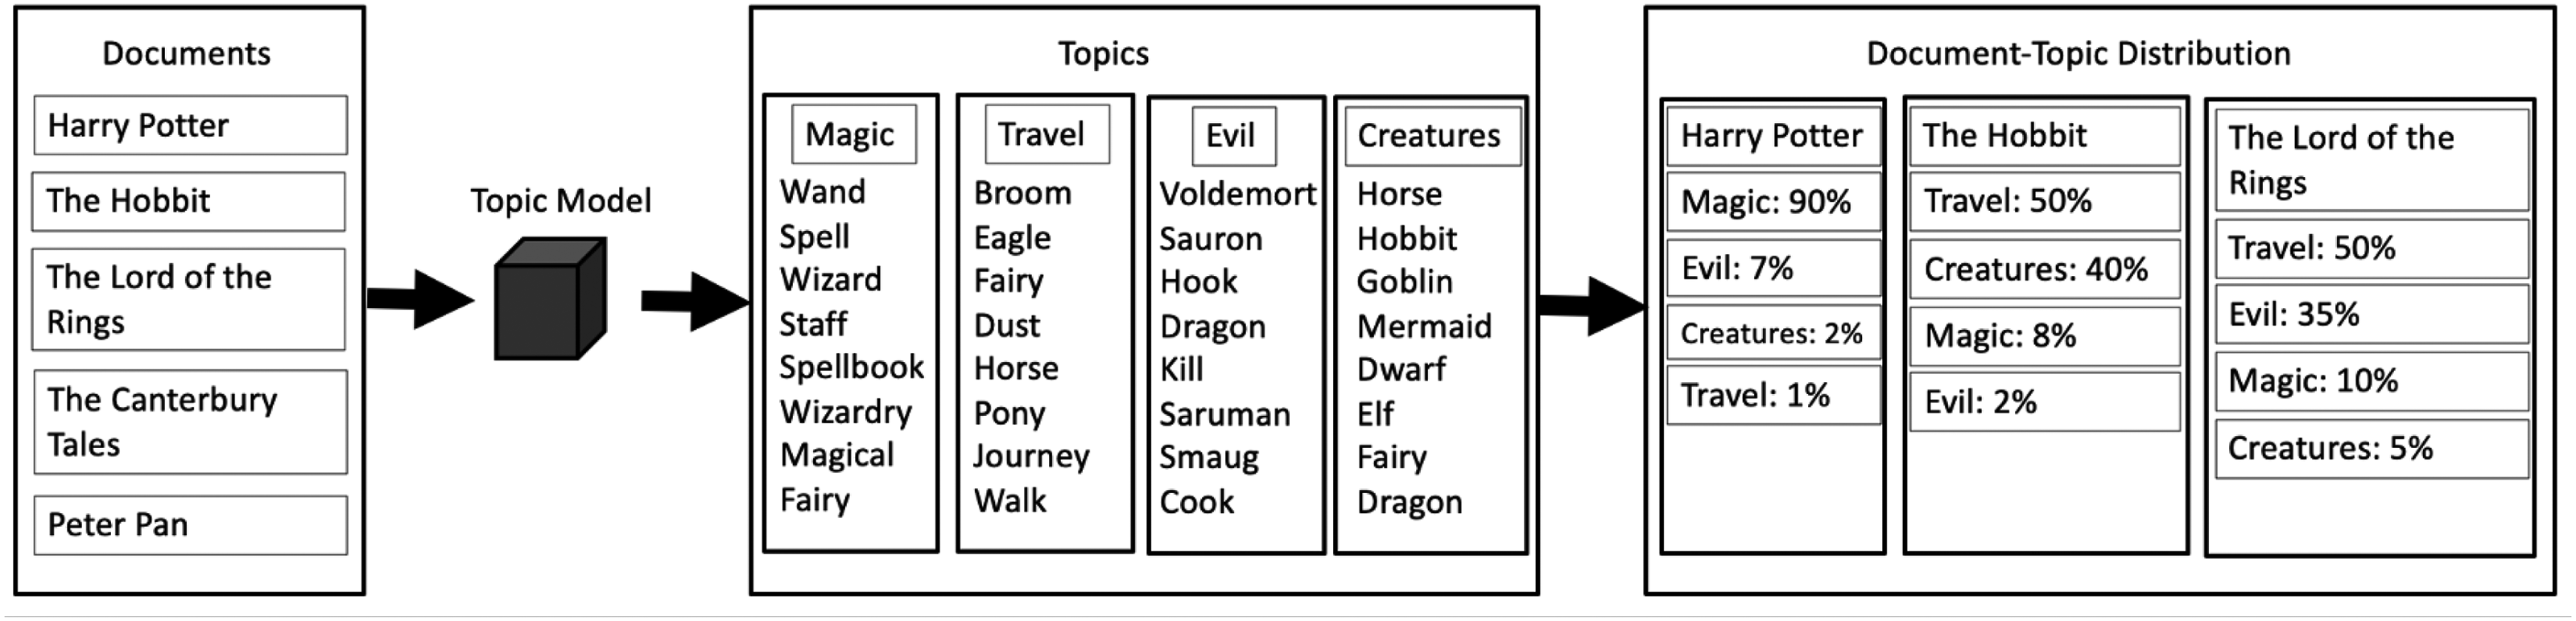
\includegraphics[trim= 0cm 0cm 0cm 0cm, clip=true, width=\textwidth]{chap1/topicModelExample.png}
    \caption{主题模型的示例} 
    \label{Chp1_1}
\end{figure}

\section{经典主题模型算法}
\subsection{潜在狄利克雷分配}
潜在狄利克雷分配(Latent Dirichlet Allocation,LDA)是一种概率主题模型,它可以给出潜在主题对应的词汇概率分布,同时给出文档集中每篇文章对应的主题概率分布。LDA也是一种词袋模型,即不考虑词与词之间的先后关系,一篇文章可以看作是词的集合。一篇文章可以有多个主题,文章中的每个词都对应一个主题。换句话说,LDA模型模拟了一篇文章的生成:先从主题集合中随机地选取一个主题,再以一定的概率从这个主题所对应的词汇集中选取一个词,不断重复上述过程,最终生成一篇文章。表\ref{MathNotationTable}描述了本节主题模型涉及概念所对应的数学符号及其说明。

\begin{table}[ht]
	\caption{在本章涉及概念对应的数学符号以及其说明}
	    \centering
	    \adjustbox{width=0.45\textwidth}{
		\begin{tabular}{cc}
		\toprule
			数学符号 & 说明  \\ 
		 \midrule
			$D$ & 语料库中文本数量  \\
			$V$ & 语料库中词表长度  \\
			$K$ & 主题数  \\ 
			$L$ & 词向量、实体向量的维度  \\   
			$N_{d}$ & 文本$d$包含的单词数  \\ 
			$w_{d,n}$ &  文本$d$中第$n$个单词 \\ 
			$z_{d,n}$ &  文本$d$中第$n$个单词的主题 \\ 
			$\vec{\theta}_{d}$ & 文本$d$对应的主题分布  \\ 
			$\vec{\alpha}$ &   $\vec\theta_{d}$狄利克雷先验超参数\\ 
			$\vec{\beta}_{k}$ & 主题$k$对应的主题-词表分布  \\ 
		   $\vec{\eta}$ &    $\vec\beta_{k}$狄利克雷先验超参数\\ 
		 \bottomrule
		\end{tabular}
		}
	\label{MathNotationTable}
\end{table}

在潜在狄利克雷分配 (LDA) 主题模型中,语料库中的一个文档 $d$ 被表示为,在 $K$ 个主题上具有狄利克雷先验的文档-主题分布 $\vec\theta_d \sim \mbox{Dirichlet}(\vec\alpha)$,而每个主题 $z$ 则通过词汇表上的主题-词分布 $\vec\beta_z\sim \mbox{Dirichlet}(\vec\eta)$ 来建模。其中狄利克雷分布的概率密度函数如公式\ref{Dirichlet}所示,
\begin{equation}
    \label{Dirichlet}
    f(x, x_2, \ldots, x_K; \vec\alpha) = \frac{\Gamma(\sum_{i=1}^K \alpha_i)}{\prod_{i=1}^K \Gamma(\alpha_i)} \prod_{i=1}^K x_i^{\alpha_i - 1}
\end{equation}
狄利克雷分布是一种连续的多变量概率分布,广泛用于概率论和统计学中,特别是作为多项分布的共轭先验分布所使用。因此,如图 \ref{lda} 所示,LDA 的生成过程描述如下:

\begin{enumerate}
    \item[(1)] 对于每一个主题 $k\in {1,\dots,K}$:
    \begin{itemize}
        \item[(a)] 采样一个主题-词分布 $\vec\beta_k\sim \mbox{Dirichlet}(\vec\eta)$ 
    \end{itemize}
	\item[(2)] 对于每一篇文档 $d \in \mathcal{D}$:
	    \begin{enumerate}
		    \item 采样一个文档-主题分布 $\vec\theta_d\sim \mbox{Dirichlet}(\vec\alpha)$
		    \item 对于 $d$ 中的每个单词 $w_{d,n}$:
		        \begin{enumerate}
			            \item 采样一个主题 $z_{d,n} \sim \mbox{Multinomial}(1,\vec\theta_d)$
			            \item 采样一个单词实体 $w_{d,n}\sim \mbox{Multinomial}(1,\vec\beta_{z_{d,n}})$
			        \end{enumerate}
		    \end{enumerate}
\end{enumerate}

\begin{figure}[ht]
    \centering
        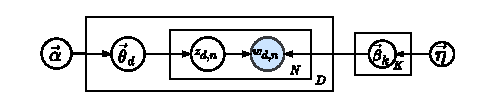
\includegraphics[width=0.8\textwidth]{chap2/LDA.pdf}
        \caption{潜在狄利克雷分配模型(LDA)的概率图模型结构} \label{lda}
\end{figure}

在这个LDA的生成框架下,文档 $d$ 的似然函数是
\begin{equation}
	\label{lda_like}
	p(d|\vec\alpha,\vec\eta)=\int_{\vec\theta_d}\left(\prod_{n=1}^{n_d}\sum_{z_n=1}^k p(z_n|\vec\theta_d)\int_{\vec\beta_k} p(w_n|z_n,\vec\beta_k)p(\vec\beta_k|\vec\eta)\dif\vec\beta_k\right)p(\vec\theta_d|\vec\alpha)\dif\vec\theta_d
\end{equation}

由于在多项式假设下文档-主题分布 $\theta$ 与主题-词分布 $\beta$ 之间的耦合性,LDA 后验推断中的隐变量 $\theta$ 和 $z$ 是难以处理的 \cite{AVITM}。因此主题模型往往采用变分推断\cite{VI}或者吉布斯采样\cite{Gibbs}进行求解。作为MCMC方法中最具有代表性的参数推断方法,吉布斯采样被广泛地应用在主题模型求解过程中。我们会在第\ref{GibbsSampling}节给出更详细的吉布斯采样介绍,这里先给出结果。在 LDA 模型中,先给每篇文章的每个词随机分配一个主题;然后循环遍历每篇文章中的每个词,此时假设当前的词隶属的主题未知,而语料库的文档中剩下的词都已明确其主题,基于此按照吉布斯采样公式计算在该词属于某一个主题的概率,并对当前的词重新采样一个主题,直到语料库的所有文章的词都被重新分配主题,不断重复上述采样过程直到模型收敛。吉布斯采样中的LDA的联合概率分布为
\begin{equation} 
	\begin{aligned}
	p(\mathcal{D},\vec{z} |\vec{\alpha},\vec{\eta}) = 
	\prod_{k=1}^K \frac{\Delta(\vec{n}_{k}+\vec{\eta})}{\Delta(\vec{\eta})}
	\prod_{d=1}^D  \frac{\Delta(\vec{n}_{d}+\vec{\alpha})}{\Delta(\vec{\alpha})}
	\end{aligned}
\label{joinProbLDA2}
\end{equation}


除了当前的单词$w$外,语料库的文档中剩下的词都已明确其主题,基于此按照吉布斯采样公式计算在该词属于某一个主题的概率为
\begin{equation} 
	p(z_w=k |\vec{z}_{\lnot w},\mathcal{D})   
	\propto  \frac{p(\mathcal{D},\vec{z} |\vec{\alpha},\vec{\eta})} 
					{p(\mathcal{D}_{\lnot w},\vec{z}_{\lnot w}|\vec{\alpha},\vec{\eta})} 
	\propto \frac{(n_{k,\lnot w}^v+\eta) }
					{\sum_{v=1}^V (n_{k,\lnot w}^v+\eta)} (n_{d,\lnot w}^k+\alpha)
\label{pzdLDA2}
\end{equation} 
其中$\Delta(\cdot)$是一个函数,例如$\Delta(\vec{\alpha}) = \frac{\prod_{k=1}^K\Gamma(\alpha)}{\Gamma(\sum_{k=1}^K \alpha)}$;$n_{k}$是主题为$k$的单词数,$n_{k}^{w}$是主题$k$下单词$w$出现的次数;$n_{d}^{k}$是文本$d$中属于主题$k$的单词数;$n_{k,\lnot w}^v$为除单词$w$外主题$k$下单词$w$的个数,$n_{d,\lnot w}^k$为除单词$w$外文章$d$属于主题$k$的单词数。

当吉布斯采样完成后,可以求解得到文档-主题分布的参数$\vec\theta$和主题-词分布的参数$\vec\beta$:
\begin{equation} 
	\begin{aligned}
	\beta_{k}^v = \frac{n_{k}^v + \eta}{\sum_{v=1}^V n_{k}^v + V\eta}
	\end{aligned}
\label{phizwLDA}
\end{equation}

\begin{equation} 
	\begin{aligned}
	\theta_{d}^k = \frac{n_{d}^k + \alpha}{\sum_{k=1}^K n_{d}^k + K \alpha}
	\end{aligned}
\label{thetadkLDA}
\end{equation}

\subsection{狄利克雷多项混合模型}
狄利克雷多项混合模型\cite{GSDMM}(Dirichlet Multinomial Mixture Model, DMM)假设数据集是包含多个主题,且每篇短文本只包含一个主题,短文本内的所有单词都由该主题生成。图\ref{DMMProbGraph}为DMM详细的生成过程。

对于整个语料库$\mathcal{D}$,DMM模型的生成式过程描述如下:
\begin{enumerate}
    	
    	\item[(1)] 采样一个语料库-主题分布$\vec{\theta} \sim \mbox{Dirichlet}(\vec{\alpha})$
    	
    	\item[(2)] 对于每一个主题 $k\in {1,\dots,K}$:
    		\begin{enumerate}
    		\item 采样一个主题-词分布 $\vec\beta_k\sim \mbox{Dirichlet}(\vec\eta)$ 
    		\end{enumerate}
    		
    	\item[(3)] 对于每一篇文档 $d \in \mathcal{D}$:
    		\begin{enumerate}
    		\item 采样一个主题$z_{d} \sim \mbox{Multinomial}(\vec{\theta})$
    		\item 对于 $d$ 中的每个单词 $w_{d,n}$:
    			\begin{enumerate}
    			\item 采样一个单词实体 $w_{d,n}\sim \mbox{Multinomial}(1,\vec\beta_{z_{d}})$
    			\end{enumerate}	
    		\end{enumerate}	 
\end{enumerate}
 
\begin{figure}[ht]
	\centering
	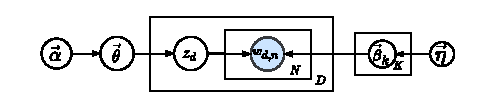
\includegraphics[width=0.8\textwidth]{chap2/DMM.pdf}\\
	\caption{狄利克雷多项混合模型(DMM)概率图模型}\label{DMMProbGraph}
\end{figure}

DMM的隐变量主题-词分布于$\vec{\beta}_{k}$和语料库-主题分布$\vec{\theta}$可以由后验分布$p(\vec{z}|d)$推理得到。同LDA的求解方法,DMM也采用吉布斯采样来求解。当除了短文本$d$外,所有其他文章的主题$\vec{z}_{\lnot d}$和所有文章$\mathcal{D}$已知时,基于吉布斯采样的参数公式如下:

\begin{equation} 
	\begin{aligned}
	p(z_d = k |\vec{z}_{\lnot d},\mathcal{D})   \propto
	\frac{n^{(k)}-1+\alpha}{D-1+K\alpha}
	\frac{\prod_{w \in d} \prod_{j=1}^{n_{d}^w}(n_{k}^w-n_{d}^w+\eta+j-1)} {\prod_{i=1}^{n_{d}}(n_{k}-n_{d}+V\eta+i-1)}
	\end{aligned}
\label{pzdDMM}
\end{equation}
其中 $n^{(k)}$是$D$篇文本中被分配给主题$k$的文章数,$n_{k}$是语料库中被分配给主题$k$的单词数,$n_{(k)}^w$是单词$w$被分配给主题$k$的次数;$n_d$是短文本$d$的长度,$n_d^w$是短文本$d$中单词$w$出现的次数。

当吉布斯采样完成后,可以求解得到文档-主题分布的参数$\vec\theta$和主题-词分布的参数$\vec\beta$:
\begin{equation} 
	\begin{aligned}
	\beta_{k}^w = \frac{n_{k}^w + \eta}{\sum_{w=1}^V n_{k}^w + V\eta}
	\end{aligned}
\label{phizw }
\end{equation}

\begin{equation} 
	\begin{aligned}
	\theta_{k} = \frac{n_{k}+\alpha}{\sum_{i=1}^K n_{i} + K\alpha}
	\end{aligned}
\label{pz-dmm}
\end{equation}

\section{吉布斯采样}\label{GibbsSampling}
上一节中主题模型的推断方法采用了吉布斯采样算法,它是马尔科夫链中随机抽取样本的一种算法。该 算法是循环采样的,同时利用了全条件概率分布来进行采样。每次采样时,只改变其中一个变量,固定其他变量,通过从某个变量相对于其他变量的条件概率分布中进行采样。具体来说,假设我们希望采样的分布由n个变量构成的$p(x_1,x_2,\dots,x_n)$,并且已经为n个变量随机选择了一个初始状态,则吉布斯采样的迭代算法如算法\ref{Gibbs}所示。
\begin{algorithm}[tb]
    \caption{吉布斯采样算法的步骤}
    \label{Gibbs}
    \LinesNumbered
    \KwIn{迭代次数 $I$}
    \KwOut{$(x_1,x_2,\dots,x_n)$的采样结果}
    随机初始化 $(x_1^{(0)},x_2^{(0)},\dots,x_n^{(0)})$\;
    \For{第$i$次迭代, $i\in 1,2,\dots,I$}{
    采样更新$x_1^{(i)}\sim p(x_1|x_2^{(i-1)},x_3^{(i-1)},\dots,x_n^{(i-1)})$\;
	采样更新$x_2^{(i)}\sim p(x_2|x_1^{(i)},x_3^{(i-1)},\dots,x_n^{(i-1)})$\;
	...\\
	采样更新$x_j^{(i)}\sim p(x_j|x_1^{(i)},x_2^{(i)},\dots,x_{j-1}^{(i)},x_{j+1}^{(i-1)},\dots,x_n^{(i-1)})$\;
	...\\
	采样更新$x_n^{(i)}\sim p(x_n|x_1^{(i)},x_2^{(i)},\dots,x_{n-1}^{(i)})$\;
    }
\end{algorithm}

在难以直接进行采样的情况下,吉布斯采样算法是一个很好的选择。该算法的思想是可以从某一个变量 的分布中抽取出一部分样本用于参数估计。上述过程中,从条件概率分布中抽取的样本可以用于近似联合概率分布的样本。

\section{基于变分自编码器的主题模型}
变分自编码器\cite{VAE}(VAE,Variational Autoencoder)是一种深度学习模型,用于无监督学习中的数据生成和编码。VAE 结合了自编码器(Autoencoder)的结构和变分推断(Variational Inference)的理论,主要用于数据的降维和生成任务。在 VAE 中,数据通过编码器映射到一个潜在空间(latent space),这个空间通常是多维高斯分布。编码器的输出不是一个固定的点,而是潜在空间中的分布参数,如均值和方差。然后从这个分布中采样,生成新的数据点,这些点通过解码器映射回原始数据空间。VAE 的关键特性是其损失函数,它包括两部分:一部分是重构误差(如均方误差),用于衡量解码数据与原始数据的相似度;另一部分是KL散度(Kullback-Leibler Divergence),用于衡量编码后的潜在分布与先验分布(通常是标准正态分布)的接近程度。这种结构使 VAE 不仅能够有效地进行数据压缩,还能生成新的、与训练数据类似的样本,应用于图像生成、风格转换等领域。

由于主题模型也可以使用变分推断的方法求解其后验分布的参数,因此一个自然的想法就是将VAE应用于LDA主题模型。如果只考虑文档-主题分布 $\theta$ 而忽略主题分配$z$以及主题-词分布的先验信息,利用符号 $\beta$ 来表示矩阵 $(\vec\beta_1,\vec\beta_2,\dots,\vec\beta_K)^{T}$,将公式\ref{lda_like}中的主题变量$z$进行积分,可以得到
\begin{equation} 
	p(d|\vec\alpha,\vec\eta)=\int_{\vec\theta_d} (\prod_{n=1}^{n_d} p(w_n|\vec\theta_d,\beta))p(\vec\theta_d|\vec\alpha)\dif\vec\theta_d
	\label{lda_like2}
\end{equation}
其中$p(w_n|\theta,\beta)$ 是一个多项式分布,使得LDA模型的生成过程变成:
\begin{enumerate}
	\item[(1)] 对于每一篇文档 $d \in \mathcal{D}$:
	    \begin{enumerate}
		    \item 采样一个文档-主题分布 $\vec\theta_d\sim \mbox{Dirichlet}(\vec\alpha)$
		    \item 对于 $d$ 中的每个单词 $w_{n}$:
		        \begin{enumerate}
			            \item 采样一个单词实体 $w_n\sim \mbox{Multinomial}(1,\vec\theta_d^{T}\beta)$
			        \end{enumerate}
		    \end{enumerate}
	\end{enumerate}
此时文档中的词将独立同分布(i.i.d)地从分布$p(x\vert\vec\theta_d;\beta)=\mbox{Multinomial}(1,\mbox{Softmax}(\vec\theta_d^{T}\beta))$中抽取,被称为“product of experts”\cite{AVITM}。

将 VAE 应用于 LDA 模型时,模型将由一个推断网络(编码器)和一个生成网络(解码器)组成。具体来说,编码器接收文档 $d$ 的词袋(BoW)表示 $x_d$ 作为输入,并输出文档-主题分布 $\theta_d \sim q(\vec\theta_d|x_d;\hat{\vec\alpha})=Dir(\hat{\vec\alpha})$,其中 $q(\vec\theta_d|x_d;\hat{\vec\alpha})$ 是真实后验 $p(\vec\theta_d|x_d)$ 的近似,通常称为变分分布;而$\hat{\vec\alpha} = f_{enc}(x_d)$ 则是通过一个多层感知机(MLP)计算得出。解码器通过给定分布 $p(w_n|\vec\theta_d,\beta)=f_{dec}(\vec\theta_d)$ ,重现接近观测值 $x_d$ 的 $\hat{x_d}$:
\begin{align}
    \hat{\vec\alpha}:&= f_{enc}(x_d;\Pi)\\
    \tilde{\vec\theta_d}&\sim q(\vec\theta_d|x_d;\hat{\vec\alpha})\\
    f_{dec}(\tilde{\vec\theta_d};\beta):&=\mbox{Softmax}(\tilde{\vec\theta_d}^{T}\beta)
\end{align}
在VAE框架下,通过最大化证据下界(ELBO)来优化编码器的参数$\Pi$和解码器的参数$\beta$:
\begin{equation} 
    \mathcal{L}(\Pi,\beta;x_d)=E_{q(\vec\theta_d|x_d)}[\log p(x_d|\vec\theta_d)]-KL(q(\vec\theta_d\vert x_d;\hat{\vec\alpha})\|p(\vec\theta_d;\vec\alpha))
\end{equation}
第一项描绘了文档BoW表示的重构误差,而第二项KL-散度作为一个正则项,使得变分分布接近先验分布。

根据随机梯度变分贝叶斯\cite{},在得到解码器的结果$\hat{\vec\alpha}$之后,需要从 $q(\vec\theta_d|x_d;\hat{\vec\alpha})$ 中采样 $\vec\theta_d$ 来估计在证据下界(ELBO)中的重构误差。通过平均多个样本的贡献来实现,如下式所示:

\begin{equation}
	\mathcal{L}(x_d)=-KL(q(\vec\theta_d|x;\hat{\vec\alpha})||p(\vec\theta_d;\vec\alpha))+\frac{1}{L}\sum_{l=1}^{L}(\log p(x_d|\vec\theta_{d,l},\beta))
	\label{elbo2}
	\end{equation}
其中 L 表示样本的数量。


随机梯度变分贝叶斯的一个基本要求是,隐变量以可微的、非中心化的参数化形式表示,以允许在优化过程中进行梯度计算。然而,狄利克雷分布的形状参数并不满足这一条件。由于狄利克雷分布可以通过伽玛随机变量来模拟,因此拒绝接受采样变分推断 \cite{RSVI} 和伽玛分布的形状增强方法被 DVAE\cite{DVAE}应用于在VAE中对狄利克雷分布进行采样。如果 $z_i \sim \mbox{Gamma}(\alpha_i, 1)$,那么 $\tilde{z}{1:K} = \frac{z{1:K}}{\Sigma_i z_i} \sim \mbox{Dir}(\alpha_{1:K})$。这一点很重要,因为存在一个高效的伽玛分布拒绝采样器:
\begin{equation}
	z=h_\Gamma(\epsilon,\alpha)=(\alpha-\frac{1}{3})(1+\frac{\epsilon}{\sqrt{9\alpha-3}})^3,\,\epsilon\sim \mbox{N}(0,1)
	\label{rejection}
\end{equation}
虽然这个函数由于有些样本会被拒绝而不等同于使用伽玛分布,但对于较高的参数 $\alpha$ 值,往往会有更高的接受率。因此可以应用拒绝采样框架\cite{RSVI}对 $\tilde{z} \sim \mbox{Gamma}(\alpha+B, 1)$ 进行采样,因为 $z \sim \mbox{Gamma}(\alpha, 1)$ 可以表示为 $z = \tilde{z} \prod_{i=1}^B u_i^{\frac{1}{\alpha+i-1}}$,其中 B 是一个正整数,且 $u_i \overset{i.i.d.}\sim \mbox{Uniform[0,1]}$。
\chapter{短文本主题模型的数据增强方法研究}\label{chap:Transferring}
\section{引言}
互联网信息媒体的徐梦发展,尤其是微博、小红书、抖音等社交媒体,带来了大量的短文本内容。如何挖掘和理解这些短文本的主题内容是许多领域的重要研究关键研究问题,例如用户兴趣分析、推荐系统和事件检测等\cite{survey_2023}。主题模型是自动将大规模文档集合压缩成内容摘要的模型,其结果表现为一系列相关单词的集合,即潜在主题。传统的主题模型,如非负矩阵分解\cite{NMF}(NMF)和潜在狄利克雷分配\cite{LDA}(LDA)等,在发现长文本中的潜在语义主题结构方面成效显著,但在短文本的应用中面临挑战。因为短文本的词汇数量有限,使得模型中在文档集中寻找单词的共现信息变得困难\cite{survey_2022},这将导致挖掘出噪声较多且缺乏连贯性的主题。

许多研究者致力于解决短文本建模中的数据稀疏性问题。一个简单的策略是使用外部元数据将短文本聚合成更长的伪文本。例如,可以使用标签、作者信息、地点和时间戳等元信息来聚合文本,然后应用LDA进行主题建模\cite{ExTwitter,PoolTwitter}。然而,这些方受限于元数据的信息,可能无法达到预期的效果。同时,这种聚合策略会减少文档数量,从而导致LDA面临文档数量较少这一问题\cite{few_documents}。BICALHO等人\cite{DREx}提出了另一种丰富单词共现模式的方法,即基于分布式表示的文本扩充方法(DREx)。DREx利用词嵌入技术从词汇表中识别相似的词汇,从而将每个短文本扩充为伪长文档。在生成伪文档之后,再对这些文档应用LDA模型。但是,根据词嵌入确定的相似词可能并不具有相同的语义,如多义词等,这将导致原始文档和伪长文档之间出现语义不一致的问题。此外,DREx仅依赖于伪长文档进行主题建模,往往会捕捉到与原始文档不一致的主题。

鉴于现有扩充方法的局限性,本章提出了一种基于提示的短文本数据增强方法。首先,我们提出了一种机制来维持短文本与伪长文本之间的语义一致性。大型语言模型(Large Language Models,LLMs)在近期展示了它们根据文本指令自动生成内容的能力\cite{glm}。受到LLMs想象力和创造力的启发,我们提出了基于提示的文本扩充方法(Instructed-Expansion,IE)。利用可以进行文本自动生成的LLMs,通过指令提示将每个短文本扩充为伪长文档。通过这种新方法,可以将LLMs的知识迁移到短文本主题建模中,而无需采集额外的辅助信息。

其次,虽然大型语言模型(LLMs)可以生成连贯的内容,但由于我们没有在目标数据集上对LLMs进行微调,IE有时会在维持原始文档主题信息的同时,带来一些额外的主题信息。因此,我们提出了一种基于短文本与伪长文本的主题模型(Text-Pairwise Topic Model,TPTM)。其假设短文本与伪长文本是一组成对数据,且短文本中的主题是从其对应伪长文本中的主题中抽取的。这种假设利用了丰富的单词共现性和短文本的独特性,以改进主题建模过程。换而言之,我们提出的TPTM使得IE方法更加灵活且便于使用。

本章工作的主要贡献概括如下:

(1)提出了一种增强短文本数据的方法,即IE方法,利用大型语言模型(LLMs)的知识将每个短文本扩充成伪长文档,用于主题建模。

(2)与以往工作不同,不单是依赖于扩充文档进行LDA主题建模,我们提出了TPTM,将伪长文档与原始短文本作为成对数据同时用于主题建模。

(3)在Tweet、SearchSnippets和StackOverflow数据集上的实验表明,相较于许多基线模型,我们提出的模型能够获得更好的主题质量和分类准确率。

% \section{短文本主题模型的数据增强方法}
% 在本节中,将介绍本章提出的主题建模框架。首先介绍我们提出的基于提示的短文本数据增强方法,它利用大型语言模型生成伪长文本。然后,我们提出了一种基于短文本与伪长文本的主题模型,该模型将伪长文档与原始短文本视为成对数据结合在主题模型中,以得到最终结果。

\section{基于提示的短文本扩充方法}
以往的研究往往将主题模型应用于文本生成这一领域。但在我们中我们采取了相反的方法,将大规模语言模型(Large Language Models,LLMs)用于辅助主题模型在短文本数据集上的建模。
LLMs,如GPT系列模型,是基于深度学习技术的先进自然语言处理工具,它们通过分析大量文本数据来理解和生成语言。这些模型通过在海量数据集上进行训练,能够捕捉到语言的复杂模式和结构,从而在文本生成任务中表现出色。LLMs的核心优势在于其能够生成连贯、有意义且常常难以区分于人类写作风格的文本。在应用方面,LLMs不仅可以高效生成文章、故事和对话,还能够进行内容摘要、自动翻译以及编写代码等。

受到LLMs丰富的想象力和创造力的启发,我们提出了基于提示的短文本数据增强方法(Instructed-Expansion,IE),使用LLMs将每个短文本扩充为一个伪长文本。具体来说,短文本中的词将被用作指导LLMs文本生成的关键词。我们将扩充后的文本称为伪长文档。通过这种方法,可以利用LLMs的外部知识缓解短文本主题建模中遇到的稀疏性问题,而无需除了短文本本身之外的任何额外标签。表\ref{expasion example} 显示了在 Tweet 数据集上,基于 Llama-2-7B\cite{llama2} 进行推断的IE方法示例,记为IE-llama2。在经过预处理后,原始文档包含了词语 "brain fluid buildup delay giffords rehab"。通过使用指令“Generate a text about 100 words based on the following words: ",IE方法获得了一个含有\textit{damage}、\textit{head}、\textit{rehabilitation}等与原文档语义相关的词来讲述故事,从而维持原始文档中的语义并增加了词的共现信息。

我们还对比了现有的另一种扩充方法,基于分布表示的扩充方法(DREx)\cite{DREx}。该方法通过词嵌入扩充短文本,即利用词嵌入计算原数据集词汇表中单词间的相似度,从而为文中单词选择相似度高的词语进行扩充。可以明显观察到我们提出的IE方法和 DREx 之间的差异。在DREx的扩充实例中,我们可以找到一些与原文本语义不相关的词,如“approve”、“push”、“pregnant”等,很难说这些词会与原文本中的单词同属于一个主题。此外,如果我们有两个短文本:“brain fluid buildup”和“pregnant stomach heart”。DREx很可能会将它们扩展为“brain fluid buildup pregnant stomach heart”和“pregnant stomach heart brain fluid buildup”。这两个扩展文本在结果上看是相同的。在某种程度上,这将减少数据集中的文档数量,并使模型认为这些词都属于同一主题。

\begin{table}
    \centering
    \caption{Tweet数据集中的一个文本示例}
    \label{expasion example}
    \adjustbox{width=\textwidth}{
    \begin{tabular}{c|l}
    \hline
    示例 & \multicolumn{1}{c}{文本内容} \\ \hline
    短文本 & brain fluid buildup delay giffords rehab \\ \hline
    \multicolumn{1}{c|}{DREx} & \begin{tabular}[c]{@{}l@{}}brain fluid buildup delay giffords rehab mixture gop supply method pregnant heart approve push \\ reaction process allow excess congresswoman detect technique avoid prevent administration adjourn \\ breathing mind halt plan require strain move liver contain force heat amount hearing rehabilitation \\ clinton affect memory announcement cause change vote stomach ongoing response scan\end{tabular} \\ \hline
    \begin{tabular}[c]{@{}c@{}}IE-llama2\end{tabular} & \begin{tabular}[c]{@{}l@{}}The brain is a complex organ that is susceptible to damage after a traumatic event such as a\\ shooting. When a bullet hits the brain, it can cause bleeding and swelling, leading to a buildup of \\fluid in the affected area. This buildup can cause delays in the healing process and can lead to further\\ damage if left untreated. In the case of former Congresswoman Gabrielle Giffords, her shooting in \\ 2011 caused significant damage to her brain, leading to a long and difficult rehabilitation process. \\Despite the challenges, Giffords has made remarkable progress and is now able to communicate and\\ function independently.
    \end{tabular} \\ \hline
    \end{tabular}
    }
\end{table}

\section{基于成对文本的主题模型}
本节首先给出一些定义。给定一个包含$D$个文档的短文本语料库$\mathbb{S}=\{S_d\}_{d=1}^D$和一个词汇表$W=\{w_1,w_2,\dots,w_V\}$。可以为$\mathbb{S}$中的每个实例使用IE方法生成一个伪文档,从而得到大小为$D$的伪文档语料库$\mathcal{P}$,表示为$\mathbb{P}=\{P_d\}_{d=1}^D$。将包含原文档和伪文档的整个数据集表示为$\mathbb{D}=\{S_d,P_d\}_{d=1}^D$。每个短文本的格式为$S_d=\{w_{d,1},w_{d,2},\dots, w_{d,M_d}\}$,其中$w_{d,n}$是$S_d$中的第$n^{th}$个词,$M_d$是$S_d$中的词数。因此,伪长文档$P_d$具有与$S_d$相同的格式,即$P_d=\{w_{d,1},w_{d,2},\dots, w_{d,N_d}\}$,其中$N_d$是$P_d$中的词数。数学符号在表\ref{notations}中解释。

\begin{table}
    \centering
    \caption{在本章涉及的数学符号及其说明}
    \label{notations}
    \adjustbox{width=0.65\textwidth}{
    {\begin{tabular}{cc}
    \toprule
    数学符号 & 说明\\
    \midrule
    $K$& 主题数量 \\
    $D$ & 短文本语料库的文本数量\\
    $V$ & 语料库中的词表长度\\
    $\mathcal{S}$ & 短文本语料库$\mathcal{S}=\{S_d\}_{d=1}^D$\\
    $\mathcal{P}$ & 伪长文本语料库$\mathcal{P}=\{P_d\}_{d=1}^D$\\
    $\mathcal{D}$ & 整个语料库$\mathbb{D}=\{S_d,P_d\}_{d=1}^D$\\
    $N_d$ & 伪长文本$P_d$包含的单词数\\
    $M_d$ & 短文本$S_d$包含的单词数\\
    $\vec\beta_k$ & 主题$k$对应的主题-词分布\\
    $\vec\eta$ & $\beta_k$的狄利克雷先验值\\
    $\vec\theta_d$ & 伪长文本$P_d$对应的文档-主题分布\\
    $\vec\alpha$ & $\theta_d$的狄利克雷先验值\\
    $z_{d,n}$ & 短文本$S_d$中第$n$个单词对应的主题编号\\
    $z_{d,n}^+$ & 伪长文本$P_d$中第$n$个单词对应的主题编号\\
    $\boldsymbol{\vec l}$ & 语料库$\mathcal{D}$中的所有单词对应的主题,$\boldsymbol{\vec l}=\{\boldsymbol{\vec z}_d^+,\boldsymbol{\vec z}_d\}_{d=1}^D$\\
    $n_{P_d}^{(k)}$ & $P_d$中属于主题$k$的单词数 \\
    $n_{S_d}^{(k)}$ & $S_d$中属于主题$k$的单词数 \\
    $n_k^{(v)}$ & 在整个语料库$\mathcal{D}$中属于主题$k$的单词数\\
    \bottomrule
    \end{tabular}}}
\end{table}

我们提出了基于成对文本的主题模型(Text-Pairwise Topic Model,TPTM)。TPTM不仅利用了伪长文档中丰富的词共现信息,还考虑了原始短文本中的内在主题。由于$S_d$和$P_d$是一一对应的,TPTM假设每个短文本$S_d$中的主题来自其对应的伪文档$P_d$。类比于新闻报道与其标题的关系,新闻标题一定体现了其报道内容的主题内容。TPTM对于短文本的生成过程可以分为两个阶段描述。第一阶段遵循LDA模型的假设来生成扩充语料库$\mathcal{P}$。在第二阶段,$S_d$中的每个词都是通过首先从$P_d$中已有的主题中采样一个主题$z$,然后从$\vec\beta_z$中采样一个词来生成的。TPTM的概率图模型如图\ref{TPTM_graph}所示,其中$\vec \alpha$和$\vec\eta$是狄利克雷先验。TPTM具体的生成过程描述如下:

\pagebreak

\begin{itemize}[]
    \item[(1)] 对于每一个主题 $k\in {1,\dots,K}$:
    \begin{itemize}
        \item[(a)] 采样一个主题-词分布 $\vec\beta_k\sim \mbox{Dirichlet}(\vec\eta)$ 
    \end{itemize}
    \item[(2)] 对于扩充后得到的每一篇伪长文本 $P_d \in \mathcal{P}$:
    \begin{itemize}
        \item[(a)] 采样一个文档-主题分布 $\vec\theta_d\sim \mbox{Dirichlet}(\vec\alpha)$
        \item[(b)] 对于 $P_d$ 中的每个单词 $w_{n}^+$:
        \begin{itemize}
            \item[i.] 采样一个主题 $z^+\sim \mbox{Multinomial}(\vec\theta_d)$
            \item[ii.] 采样一个单词实体 $w_{n}^+\sim \mbox{Multinomial}(\vec\beta_{z^+})$
        \end{itemize}
    \end{itemize}
    \item[(3)] 对于原来的每一篇短文本 $S_d \in \mathcal{S}$:
    \begin{itemize}
        \item[(a)] 对于 $S_d$ 中的每个单词 $w_{n}$:
        \begin{itemize}
            \item[i.] 从$P_d$的主题$\{z_{d,n}^+\}_{n=1}^{N_d}$中采样一个主题$z$
            \item[ii.] 采样一个单词实体$w_{n}\sim \mbox{Multinomial}(\vec\beta_z)$
        \end{itemize}
    \end{itemize}
\end{itemize}

\begin{figure}[ht]
    \centering
    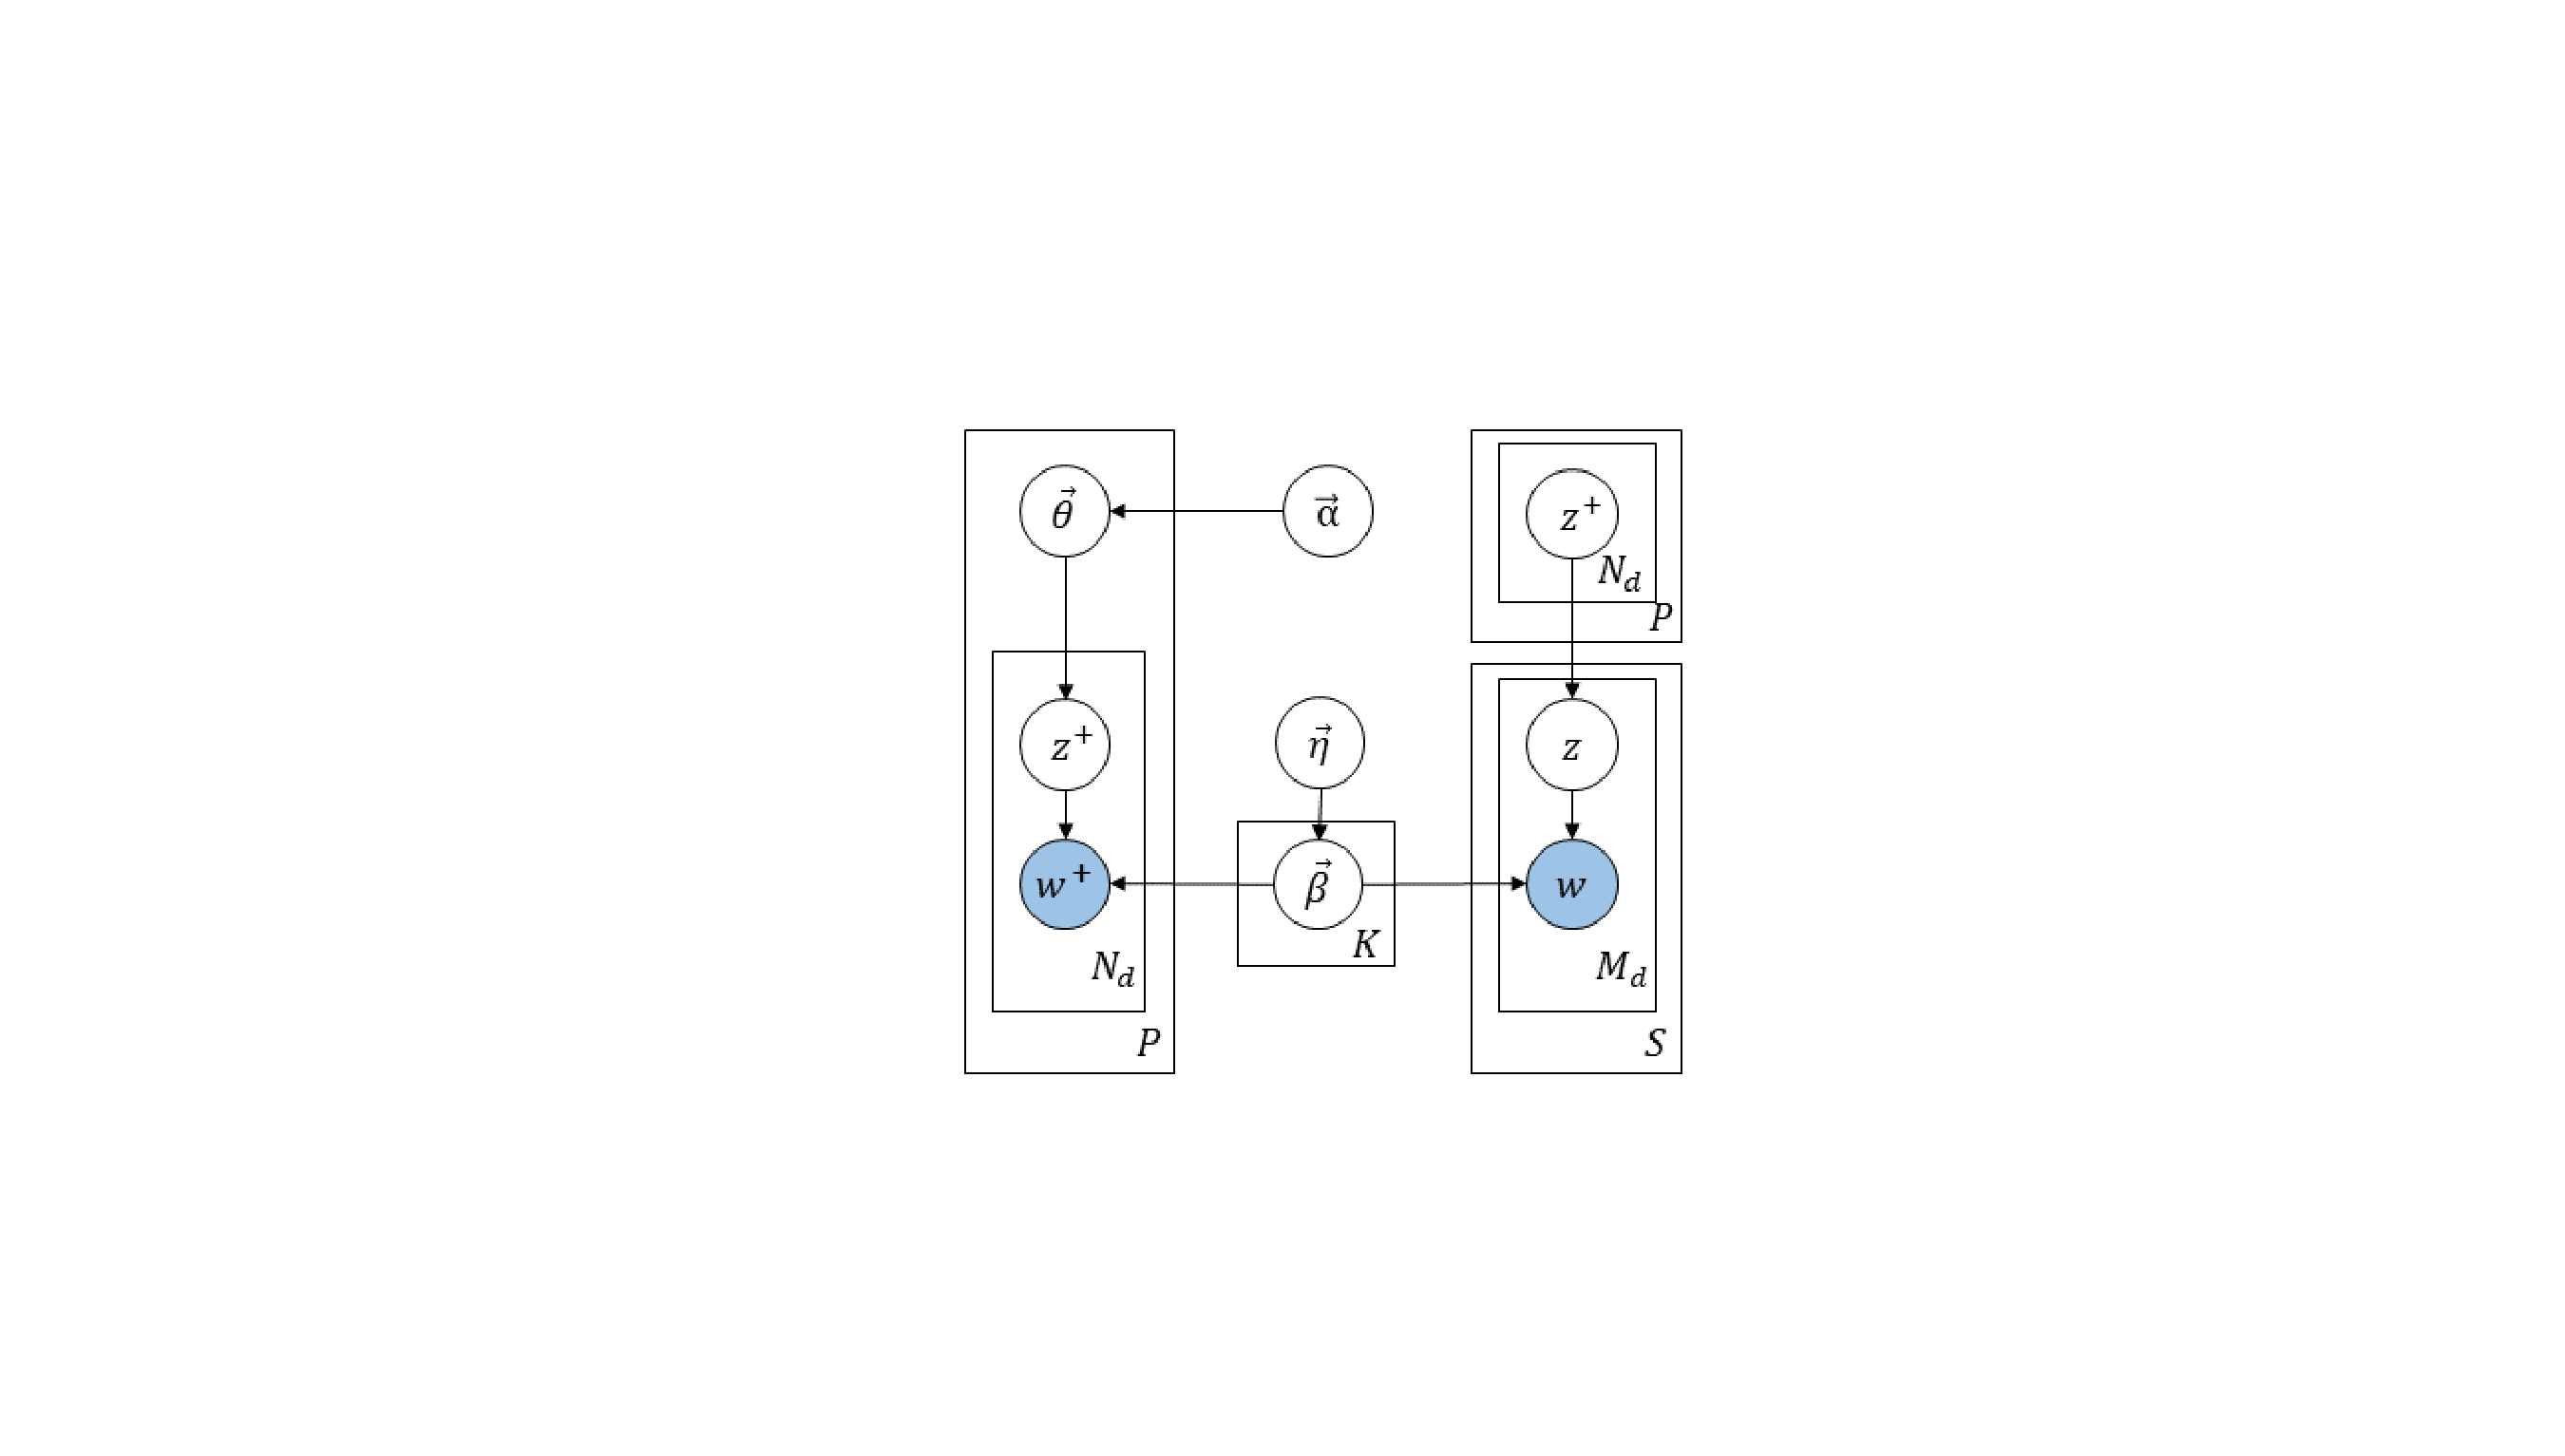
\includegraphics[trim= 15cm 5cm 15cm 5cm, clip=true, width=0.5\textwidth]{chap3/IETM.eps}
    \caption{基于成对文本的主题模型(TPTM)的概率图模型} 
    \label{TPTM_graph}
\end{figure}

\section{模型推断}
给定语料库$\mathbb{S}$和扩充语料库$\mathbb{P}$之后,需要推导出生成模型的后验分布。然而,精确的后验分布推断是不可求解的。同大部分主题模型一样,我们采用吉布斯采样算法进行后验推断。根据图\ref{TPTM_graph}中的基于成对文本的主题模型生成模型,通过对$\theta$和$\beta$进行积分,可以得到每个词对应主题的条件后验概率分布,以执行推断过程。吉布斯采样算法的详细细节可以在算法\ref{Gibbs_algo}中找到。图\ref{OverallFramework}中描绘了主题的采样过程。在每次迭代中,对于一篇伪长文档,将根据当前的主题-词分布以及这一篇文档对应的主题分布,为每个词采样一个主题。然后,为短文本中的每个词,通用利用当前的主题-词分布,从出现在其对应伪长文档中的主题中采样一个主题。

\begin{figure}[ht]
    \centering
    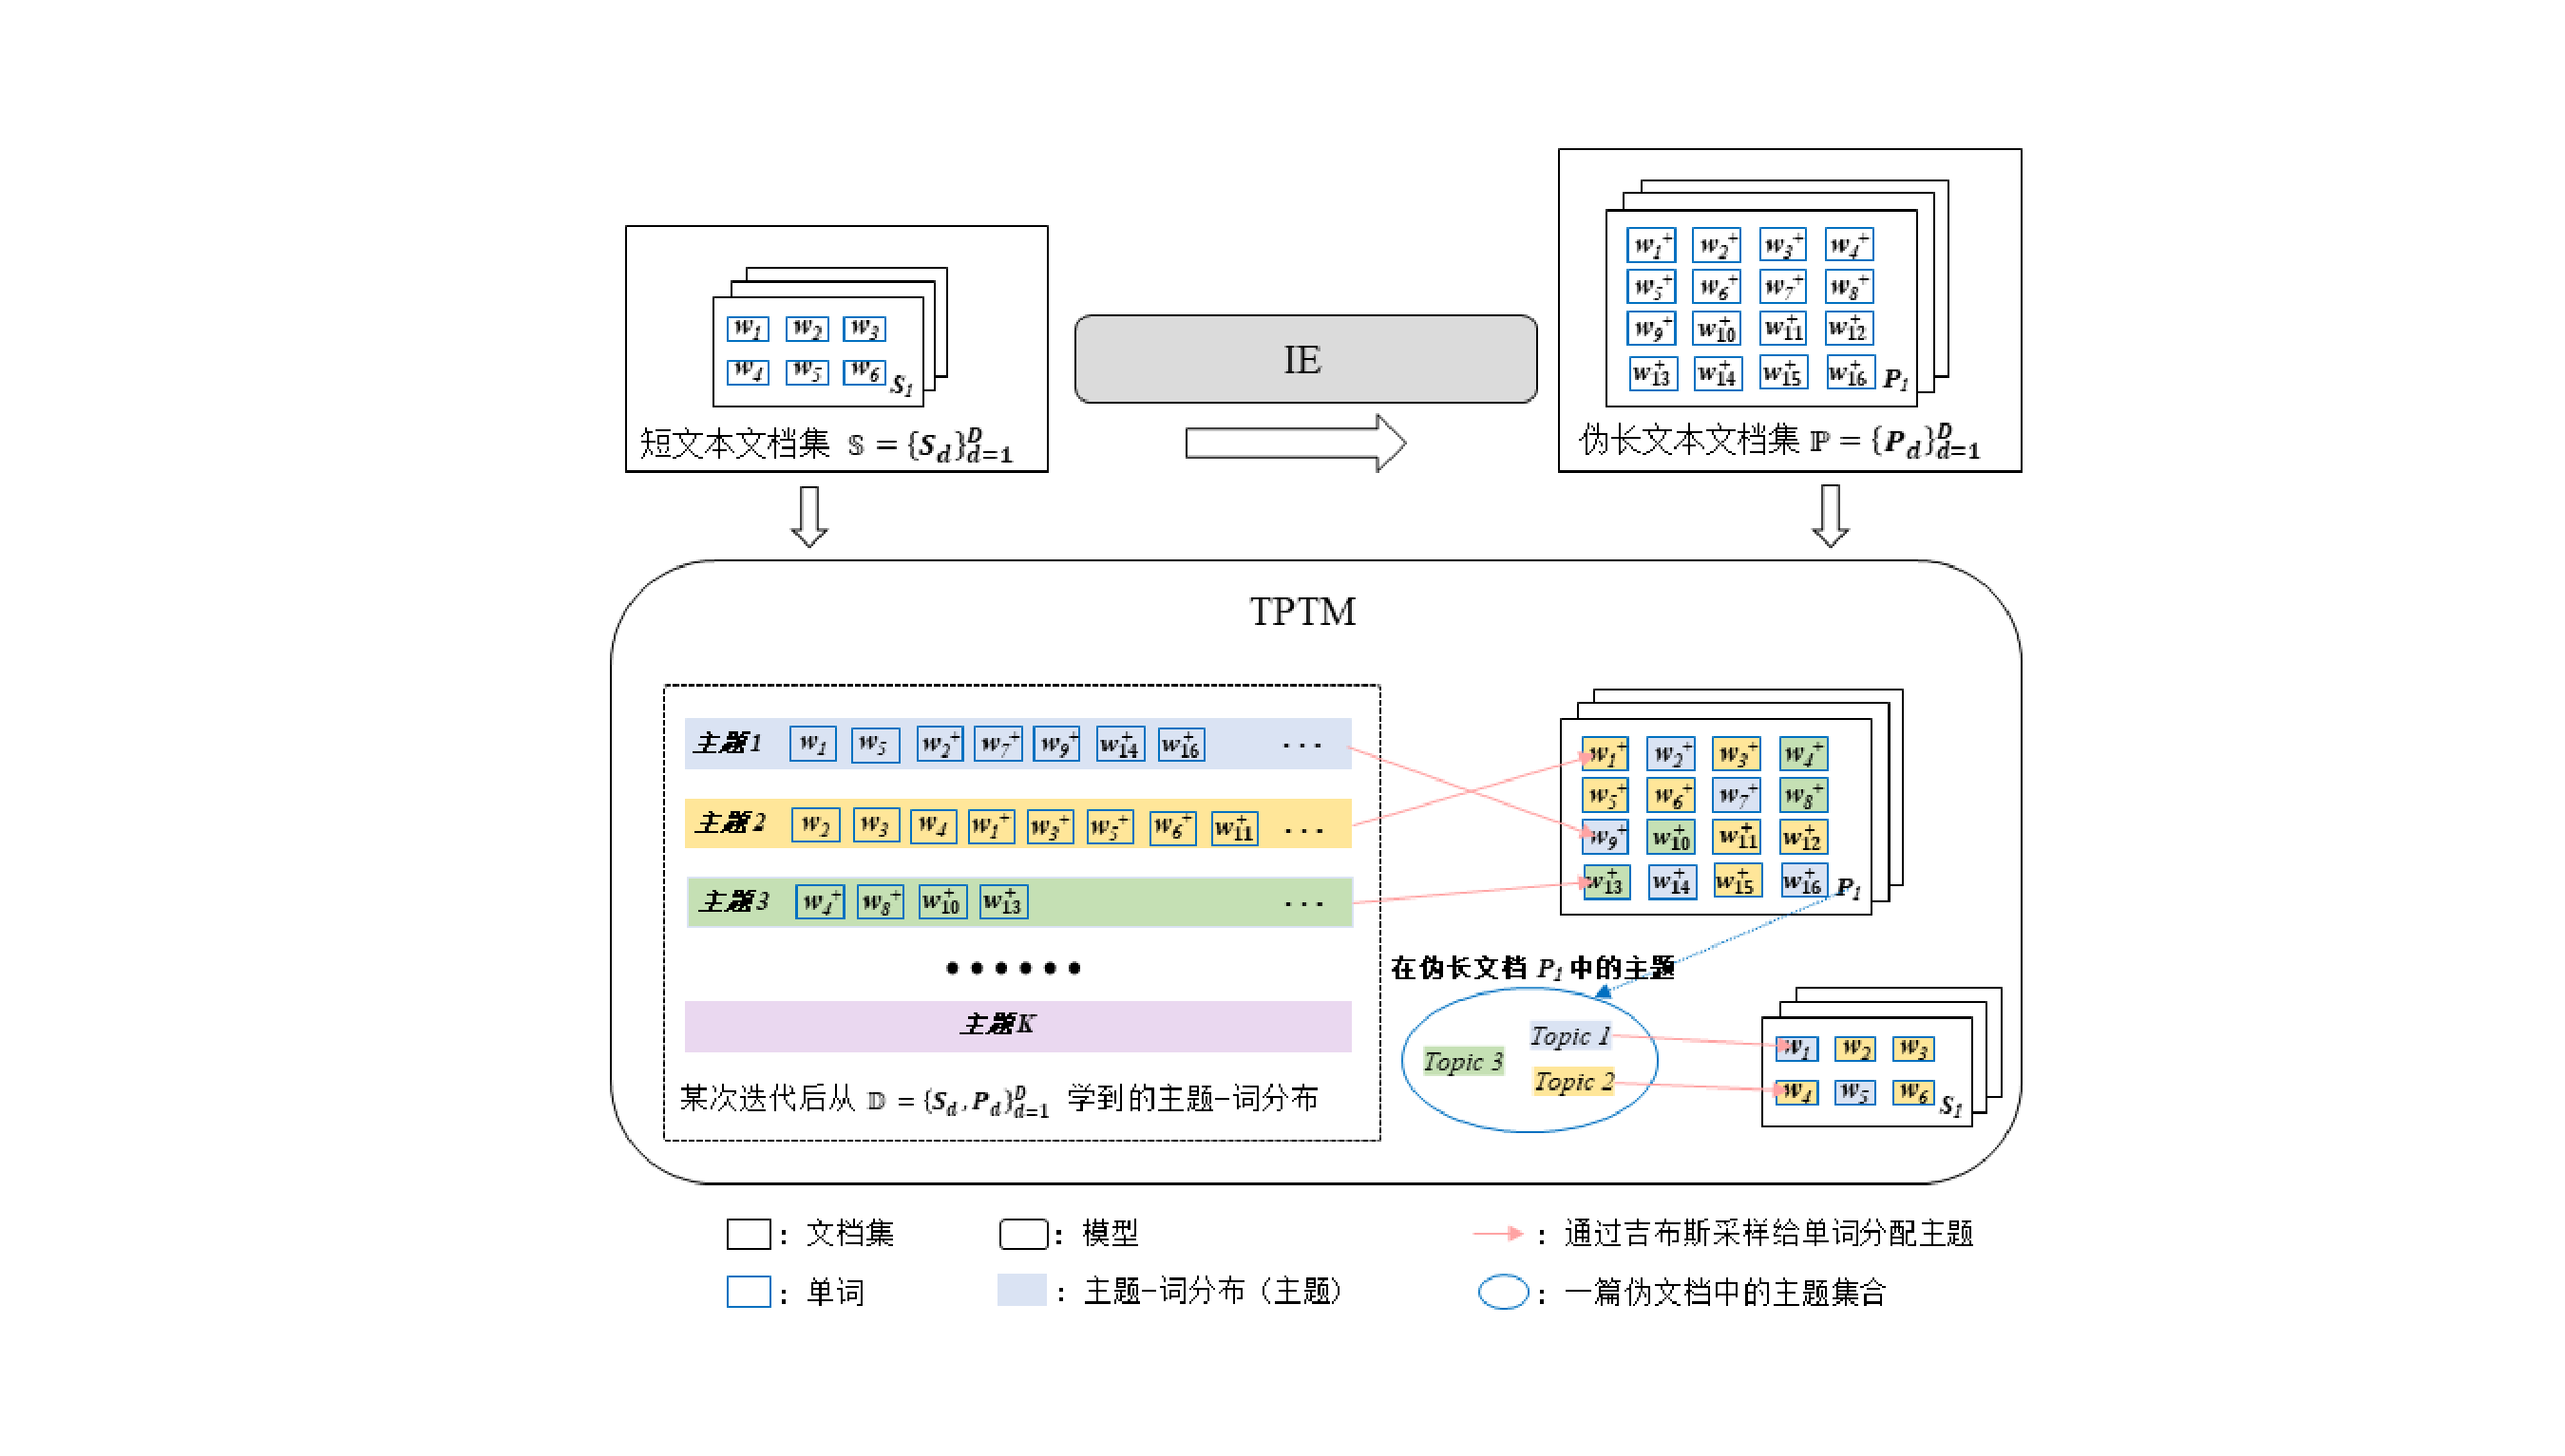
\includegraphics[trim= 10cm 2cm 8cm 2cm, clip=true, width=\textwidth]{chap3/Structure.eps}
    \caption{整体框架示意图} 
    \label{OverallFramework}
\end{figure}

\begin{algorithm}[tb]
    \caption{TPTM的吉布斯采样过程}
    \label{Gibbs_algo}
    \LinesNumbered
    \KwIn{$K$, $\alpha$, $\eta$, 文档集 $\mathcal{S}$, $\mathcal{P}$ 以及迭代次数 $I$}
    \KwOut{主题分配 $\vec{z}$ 和 $\vec{z}^+$; 主题-词的后验分布 $\beta$}
    随机初始化 $\vec{z}^+$\;
    根据 $\vec{z}^+$ 随机初始化 $\vec{z}$ \;
    初始化计数变量 $n_{P_d}^{(k)}$, $n_{S_d}^{(k)}$, $n_k^{(v)}$\;
    \For{第$i$次迭代, $i\in 1,2,\dots,I$}{
    \For{伪长文档$P_d$,$P_d\in \mathcal{P}$}{
    \For{$P_d$中的每一个单词, $w_{d,n}^+\in P_d$}{
    根据Eq.(\ref{sample1})采样一个主题$z_{d,n}^+$分配给单词$w_{d,n}^+$\;
    }
    }
    \For{短文本$S_d$,$S_d\in \mathcal{S}$}{
    \For{$S_d$中的每一个单词,$w_{d,n}\in S_d$}{
    根据Eq.(\ref{sample2})采样一个主题$z_{d,n}$分配给单词$w_{d,n}$\;
    }
    }
    }
\end{algorithm}

在吉布斯采样过程中,我们需要求解TPTM两个条件后验概率分布:(1)为伪文档$P_d$中的词$w_{d,n}^+$采样一个主题$z_{d,n}^+$的条件后验概率分布;(2)对于原始文档$S_d$中的词$w_{d,n}$,将采样一个主题$z_{d,n}$条件后验概率分布。推导过程与细节见附录A。
对于(1),我们有
\begin{equation}
\label{sample1}
\begin{aligned}
    &p(z_{d,n}^+=k|\boldsymbol{\vec l}_{\neg(P_{d,n})},\mathcal{D})\propto\\
    &\frac{n_{k,\neg(P_{d,n})}^{(v)}+\eta}{\sum_{i=1}^V(n_{k,\neg(P_{d,n})}^{(i)}+\eta)}
    \cdot\frac{n_{P_d,\neg(P_{d,n})}^{(k)}+\alpha}{N_d-1+K\alpha}\cdot\left(\frac{N_d-1}{N_d}\cdot\frac{n_{P_d,\neg(P_{d,n})}^{(k)}+1}{n_{P_d,\neg(P_{d,n})}^{(k)}}\right)^{n_{S_d}^{(k)}}
    \end{aligned}
\end{equation}
其中$\boldsymbol{\vec l}=\{\boldsymbol{\vec l}_d\}_{d=1}^D=\{\boldsymbol{\vec z}^+, \boldsymbol{\vec z}\}=\{\boldsymbol{\vec z}_d^+,\boldsymbol{\vec z}_d\}_{d=1}^D$。$n_{P_d}^{(k)}$ 和 $n_{S_d}^{(k)}$ 分别是第 $d$ 个伪文档和原始文档中属于第 $k$ 个主题的词的数量。而 $n_k^{(v)}$ 是分配给 $\mathcal{D}$ 中第 $k$ 个主题的词 $v$ 的出现次数。所有带有 $\neg\bullet$ 的计数表示排除来自 $\bullet$ 的计数。

类似地,对于(2),原始文档$S_d$中的词$w_{d,n}$,其采样一个主题$z_{d,n}$的条件后验概率分布为公式(\ref{sample2})为
\begin{equation}
    \begin{aligned}
    \label{sample2}
    p(z_{d,n}=k|\boldsymbol{\vec l}_{\neg(S_{d,n})},\mathcal{D})
    \propto\frac{n_{k,\neg(S_{d,n})}^{(v)}+\eta}{\sum_{i=1}^V(n_{k,\neg(S_{d,n})}^{(i)}+\eta)}\cdot\left(\frac{n_{P_d}^{(k)}}{N_d}\right)
    \end{aligned}
\end{equation}

显然,在这两个采样方程中,将伪文档作为辅助信息有助于提高短文本的主题学习。另一方面,我们还通过使用来自相应短文本的信息来增强伪文档的主题学习。此外,在采样迭代过程中,$n_{P_d,\neg(P_{d,n})}^{(k)}$ 可能等于零。当 $n_{P_d,\neg(P_{d,n})}^{(k)}=0$ 时,我们将公式(\ref{sample1})中的第三项设为1。

TPTM在一次迭代中需要为整个语料库$\mathcal{D}$中的每一个词都采样一次主题,所以TPTM的时间复杂度为$O(KW)$,其中$K$是主题数,$W$是整个语料库$\mathcal{D}$中的总词数。可以看出TPTM有着与LDA模型相同的时间复杂度。经过吉布斯采样迭代后,我们可以估计主题-词分布$\vec{\beta}_k$,如公式(\ref{beta})所示,从而获得最终的潜在主题。

\begin{equation}
    \label{beta}
    \beta_{k,v}=\frac{n_k^{(v)}+\eta}{\sum_{i=1}^V(n_k^{(i)}+\eta)}
\end{equation} 

\section{讨论}
TPTM利用短文本和伪文档之间存在的单词共现模式来挖掘主题。因此,TPTM在很大程度上缓解了短文本中单词共现信息的不足。另一种提高短文本建模性能的可行方法是仅依赖扩充后的伪文档来训练LDA模型。然而,由于原始文档和伪文档之间可能存在的不一致性,这种方法可能会忽略甚至消除短文本中的独特信息。与此相反,TPTM将原始文档和其伪文档视为两个不同但几乎具有相同语义的数据集进行主题挖掘。

TPTM从扩展文档中抽取主题的思想是新颖的。不过,TPTM的概率图模型结构类似于自聚合主题模型(SATM)\cite{SATM}。在标准主题建模中,SATM假设每个短文本都是从一个未观察到的长伪文档中抽样得来的,并从中推断出潜在主题。相反,在本文中,我们可以获得用于主题建模的每个伪文档的具体内容。此外,SATM直接从伪文档中的词汇中抽样短文本中的词汇,而TPTM首先为短文本抽样主题,然后从主题-词分布中抽样词汇。因此,TPTM放宽了SATM中的假设,使其在建模短文本时更加合理和灵活。

此外,我们希望探讨TPTM与COTM\cite{COTM}之间的相似性和差异性。COTM是为建模短文本而设计的,这些短文本的特点是它们与通常较长的普通文档共现。例如,一个新闻文章后面可能跟着多条用户评论。因此,COTM是一种一对多的模型,并且短文本中的内容可能与其对应的普通文档讨论不同的主题。然而,在TPTM中,通过Instructed-Expansion方法,可以获得与原始文档几乎完全相同语义的伪文档。由于TPTM是一对一的模型,我们不必担心这原语料库与伪文档语料库之间的语义不一致。更重要的是,许多短文本模型的难点在于缺乏与它们对应的普通文档或辅助信息。但在本文中,我们可以通过大型语言模型(LLMs)生成伪文档,并使用TPTM更好地建模原始语料库与扩展语料库之间的关联。

\section{实验设置}
本节基于现实生活中的短文本数据集,同许多短文本主题模型一起进行了一系列的实验,以评估本章提出的短文本扩充方法及主题模型的有效性。

\subsection{数据集}
本章采用了三个真实的短文本数据集进行实验分析,分别是:(1)Tweet\cite{GSDMM}数据集,包含2,472个推文,涵盖了89个类别;(2)SearchSnippets数据集,包含来自8个不同领域的网络搜索片段\cite{SearchSnippets}。(3)StackOverflow数据集,包含从20个不同领域的问题中随机选择的20,000个问题的标题\cite{SearchSnippets}。

对于所有数据集,我们进行了以下预处理步骤:(1)将字母转换为小写;(2)去除非拉丁字符和停用词;(3)利用NLTK的WordNet词形还原器的单词进行词干提取;(4)过滤掉长度小于2的短文本。我们采用GPT-3.5(text-davinci-003)\cite{GPT3}、配置了Low-Rank Adaptation(LoRA)\cite{lora} 的Llama-7b\cite{llama}, 以及Llama2-7b-chat\cite{llama2},应用于我们提出的Instructed-Expansion方法,分别记为IE-GPT、IE-llama和IE-llama2。使用指令:“Generate a text about 100 words based on the following words:”,并结合预处理后的短文本中的词汇,我们获得了扩展后的伪文档数据集。对于伪文档数据集,还有一个额外的预处理步骤,即移除不在原始语料库中的单词。每个数据集预处理后的统计数据汇总在表\ref{TableCopusInformation}中,其中$D$代表每个数据集中的文档数量,$V$表示词汇表的大小,$C$指数据集中的类别数量,$N$表示语料库中文本的平均长度。最后三行是不同大模型得到的伪长文档集的平均长度。

\begin{table}
    \centering
    \caption{数据集的基本信息}
    \label{TableCopusInformation}
    \adjustbox{width=0.55\textwidth}{
        \begin{tabular}{lccc}
        \hline
        数据集  & Tweet & SearchSnippets & StackOverflow \\ \hline
        $D$        & 2,472  & 12,295          & 16,407         \\
        $V$        & 4,758  & 3,803           & 1,682          \\
        $C$        & 89    & 8              & 20            \\
        短文本-$N$ & 8.5   & 14.4           & 4.8           \\
        IE-GPT-$N$   & 44.1  & 47.1           & 49.2          \\
        IE-llama-$N$ & 40.3  & 43.4           & 49.2          \\
        IE-llama2-$N$   & 42.4     & 50.9        & 38.7        \\\hline
        \end{tabular}
        }
\end{table}

\subsection{对比模型}
为了验证我们提出的短文本主题模型的有效性,本节将所提出的模型与多种现有模型进行对比并根据评价指标来分析结果,参与对比的模型有(1)LDA模型; (2)基于DMM的模型:DMM模型、GPUDMM模型、MultiKE-DMM模型和TSSE-DMM模型;(3)基于文本自聚合的模型:PTM模型和PYSTM模型;(4)BTM模型和SeaNMF模型。对比模型的详细介绍如下:

\textbf{(1)LDA\cite{LDA}:}该方法以狄利克雷分布作为先验分布,将每个文档视为主题的概率分布,每个主题则视为词汇的概率分布,通过推断这些分布的后验分布来揭示文档的潜在主题内容。

\textbf{(2)DMM\cite{GSDMM}:}该模型假设每篇文档由单一主题生成。它基于Dirichlet分布指派文档至特定主题,并通过多项分布来确定该主题下的词汇分布,从而揭示文档的主要主题。

\textbf{(3)GPUDMM\cite{GPUDMM}:}该模型是基于外部知识的方法,利用广义波利亚罐模型将词向量引入DMM模型中,以增强DMM模型的主题挖掘能力

\textbf{(4)MultiKE-DMM\cite{MKEDMM}:}引入词向量与知识图谱两种外部知识,构建多知识加权的词表示向量,并利用多知识融合的度量方法来捕捉单词更全面的相互关系。

\textbf{(5)TSSE-DMM\cite{TSSE}:}通过语义增强机制,提高模型对短文本中稀疏特征的处理能力,从而更有效地识别和区分主题。

\textbf{(6)PTM\cite{PTM}:}该模型将相关的短文本组合成一个较长的伪文档,以隐式地增加数据的丰富性和上下文信息,从而改善主题模型在处理短文本时的表现和准确性。

\textbf{(7)PYSTM\cite{PYSTM}:}该模型通过从Dirichlet过程中采样来参数化PTM模型中伪长文本的数量,能够灵活地考虑多少短文本是出自于一个伪长文本。

\textbf{(8)BTM\cite{BTM}:}该模型基于“biterms”(文档中词对的集合)而非整个文档或单个词来建模,从而直接捕捉词汇间的共现模式。

\textbf{(9)SeaNMF\cite{SeaNMF}:}该模型通过非负矩阵分解,将短文本集的上下文语义和词嵌入信息引入模型中。

\subsection{参数设置}
所有基准模型的参数值都按照其作者在论文中的推荐值设置。我们为TPTM选择了$\alpha=1.0$ 和 $\beta=0.01$。同时将所有对比模型的迭代次数设定为2,000次。 每个模型在每个数据集上都会运行5次,并记录其平均值作为最终结果。由于主题建模是一种无监督学习方法,对于主题数的设置没有一个很好的参考。在本节中,实验中所有模型的主题数量都设定为$K=25, 50$。

\subsection{评估指标}
为了对实验结果进行评估,我们专注于两个常用的评估指标:主题一致性和主题多样性。主题一致性是衡量主题可解释性的定量指标。在计算主题一致性时,需要使用外部数据集来根据术语共现为词对打分。我们采用标准化点互信息(Normalized Pointwise Mutual Information,NPMI)\cite{coherence} 来评估模型所挖掘出的主题在外部的语料库(英文维基百科文章)上的主题一致性。NPMI 暗示了一个主题的最可能单词倾向于在同一文档中共同出现。给定一个主题 $k$ 及其概率最高的前 $T$ 个单词 $(w_1,w_2,\dots,w_T)$,主题 $k$ 的 NPMI 为:
\begin{equation}
    \mbox{NPMI}(k)=\sum_{j=2}^T\sum_{i=1}^{j-1}-\frac{\log\frac{P(w_i,w_j)}{P(w_i)P(w_j)}}{\log P(w_i,w_j)}
 \end{equation}
其中 $p(w_i)$ 是单词 $w_i$ 出现在文档中的概率,$p(w_i,w_j)$ 是单词 $w_i$ 和 $w_j$ 同时出现在同一文档中的概率。NPMI数值越大意味着一个主题中的单词倾向于在同一文档内共同出现。本节计算所有主题前5、10和15个词的NPMI平均值作为最终结果。

主题多样性对应于每个词在同一模型的其他主题中出现的平均概率\cite{DVAE}。本节对所有主题的前15个词使用主题独特性(Topic Unique,TU)进行度量\cite{TU}。对于主题 $K$ 的前 $T$ 个单词,它被定义为
\begin{equation}
    TU(k) = \frac{1}{T}\sum_{i=1}^T\frac{1}{cnt(w_i)}
\end{equation}
其中 $cnt(w_i)$ 是单词 $w_i$ 在所有主题的前 $T$ 个单词中出现的总次数。TU接近1表示主题更加多样化,接近0则表示这个主题重复出现,是冗余的。

直观上,较高的NPMI通常会导致较低的TU,因为一致的主题倾向于被重复发现,而较高的TU则会带来较低的NPMI,因为其鼓励发现更多边缘主题\cite{NQTM}。因此,我们更倾向于在上述两个方面之间取得良好平衡的主题。为了衡量这一点,与Adji等人\cite{overallQuality,iclr/0003G0ZTCZ22}相同,我们采用了主题质量(Topic Quality,TQ)分数作为总体评估的指标,该得分被定义为NPMI和TU值的乘积,$\mbox{TQ}=\mbox{NPMI}\times \mbox{TU}$。%对于所有指标,$t$检验显示SpareNTM与每个基线之间的性能差异在平均值方面是否具有统计学显著性。如果从$t$检验中得到的$P$值低于0.05,我们认为成对性能差异是显著的。

\section{实验结果与分析}
\label{experiment_r}

\subsection{主题质量评估}
本节将TPTM的实验结果与其他基线模型进行对比分析。TPTM-GPT、TPTM-llama和TPTM-llama2分别代表使用IE-GPT、IE-llama和IE-llama2的TPTM。如表\ref{TableTopicQuality50}和\ref{TableTopicQuality100}所示,可以观察到,我们提出的TPTM-llama2在所有三个数据集中几乎都取得了最佳的主题质量(TQ)得分。这验证了TPTM-llama2在主题一致性和多样性之间达到了比其他基线更好且更均衡的主题质量。从表\ref{TableTopicQuality50}和表\ref{TableTopicQuality100}也可以看到,DREx相比于其他基线模型获得了最佳的主题质量,尤其是在NPMI方面。由于DREx通过使用词嵌入来选择词汇表中的相似词来扩展短文本,所以相似词共享相同主题这一点是直观的,这确实提高了主题一致性。不幸的是,DREx容易产生重复主题。这是因为DREx会模糊主题之间的区别。例如,如果我们有两个短文本:“brain fluid buildup”和“pregnant stomach heart”,我们不能简单地将这些词视为属于同一主题。然而,DREx可能会将它们扩展为“brain fluid buildup pregnant stomach heart”和“pregnant stomach heart brain fluid buildup”。这两个扩展文本在结果上看是相同的。在某种程度上,这将减少数据集中的文档数量,并使模型认为这些词都属于同一主题。此外,在基于DMM的模型中,GPUDMM和MultiKE-DMM因为使用了外部知识取得了更好的结果。基于上述分析,可以证明本文提出的TPTM成功地通过从LLMs转移知识,为短文本数据集挖掘出了更高质量的潜在主题。

\begin{table}[ht]
    \centering
    \caption{当主题数为25时的主题质量,其中加粗表示最好的结果}
    \label{TableTopicQuality50}
    \adjustbox{width=0.85\textwidth}{
    \begin{tabular}{lccc|ccc|ccc}
    \hline
    \multicolumn{1}{c}{\multirow{2}{*}{模型}} & \multicolumn{3}{c|}{Tweet} & \multicolumn{3}{c|}{SearchSnippets} & \multicolumn{3}{c}{StackOverflow} \\
    \multicolumn{1}{c}{} & NPMI & TU & \textbf{TQ} & NPMI & TU & \textbf{TQ} & NPMI & TU & \textbf{TQ} \\\hline
    LDA         & 0.187          & 0.872          & 0.163          & 0.234          & 0.799          & 0.187          & 0.212          & 0.592          & 0.126          \\
    BTM         & 0.186          & 0.758          & 0.141          & 0.245          & 0.668          & 0.164          & 0.196          & 0.357          & 0.070          \\
    SeaNMF      & 0.178          & \textbf{0.966} & 0.172          & 0.250          & 0.776          & 0.194          & 0.199          & 0.605          & 0.120          \\
    DMM         & 0.191          & 0.822          & 0.157          & 0.244          & 0.675          & 0.165          & 0.195          & 0.430          & 0.084          \\
    GPUDMM      & 0.196          & 0.751          & 0.147          & 0.25           & 0.725          & 0.183          & 0.201          & 0.360          & 0.072          \\
    TSSE-DMM    & 0.198          & 0.714          & 0.141          & 0.225          & 0.569          & 0.128          & 0.188          & 0.457          & 0.086          \\
    MultiKE-DMM & 0.190          & 0.792          & 0.150          & 0.219          & 0.745          & 0.163          & 0.163          & 0.418          & 0.068          \\
    PTM         & 0.184          & 0.813          & 0.150          & 0.240          & 0.772          & 0.185          & 0.211          & 0.577          & 0.122          \\
    PYSTM       & 0.184          & 0.853          & 0.157          & 0.233          & 0.851          & 0.198          & 0.195          & 0.725          & 0.141          \\
    DREx        & \textbf{0.262} & 0.793          & \textbf{0.207} & \textbf{0.283} & 0.744          & 0.210          & \textbf{0.279} & 0.586          & 0.163          \\\hline
    TPTM-GPT    & 0.223          & 0.818          & 0.182          & 0.252          & 0.889          & 0.224          & 0.242          & 0.727          & 0.176          \\
    TPTM-llama  & 0.216          & 0.905          & 0.195          & 0.246          & \textbf{0.965} & \textbf{0.237} & 0.224          & \textbf{0.893} &\textbf{0.200}  \\
    TPTM-llama2 & 0.230          & 0.877          & 0.202          & 0.265          & 0.878          & \textbf{0.237} & 0.238          & 0.789          &\textbf{0.200}   \\\hline
    \end{tabular}
    }
\end{table}
    
\begin{table}[ht]
    \centering 
    \caption{当主题数为50时的主题质量,其中加粗表示最好的结果}
    \label{TableTopicQuality100}
    \adjustbox{width=0.85\textwidth}{
    \begin{tabular}{lccc|ccc|ccc}
        \hline
        \multicolumn{1}{c}{\multirow{2}{*}{模型}} & \multicolumn{3}{c|}{Tweet} & \multicolumn{3}{c|}{SearchSnippets} & \multicolumn{3}{c}{StackOverflow} \\
        \multicolumn{1}{c}{} & NPMI & TU & \textbf{TQ} & NPMI & TU & \textbf{TQ} & NPMI & TU & \textbf{TQ} \\\hline
        LDA & 0.184 & 0.810 & 0.149 & 0.225 & 0.723 & 0.163 & 0.200 & 0.605 & 0.121 \\
        BTM & 0.181 & 0.641 & 0.116 & 0.241 & 0.562 & 0.135 & 0.192 & 0.294 & 0.056 \\
        SeaNMF & 0.162 & 0.925 & 0.150 & 0.248 & 0.747 & 0.185 & 0.180 & 0.581 & 0.105 \\
        DMM & 0.206 & 0.580 & 0.119 & 0.240 & 0.546 & 0.131 & 0.197 & 0.415 & 0.082 \\
        GPUDMM & 0.189 & 0.579 & 0.109 & 0.242 & 0.571 & 0.138 & 0.194 & 0.255 & 0.049 \\
        TSSE-DMM & 0.200 & 0.643 & 0.129 & 0.223 & 0.458 & 0.102 & 0.187 & 0.534 & 0.100 \\
        MultiKE-DMM & 0.190 & 0.672 & 0.128 & 0.205 & 0.629 & 0.129 & 0.150 & 0.359 & 0.054 \\
        PTM & 0.183 & 0.746 & 0.137 & 0.225 & 0.650 & 0.146 & 0.211 & 0.516 & 0.109 \\
        PYSTM & 0.181 & 0.750 & 0.136 & 0.226 & 0.748 & 0.169 & 0.189 & 0.637 & 0.120 \\
        DREx & \textbf{0.257} & 0.737 & 0.189 & \textbf{0.282} & 0.664 & 0.187 & \textbf{0.276} & 0.442 & 0.122 \\\hline
        TPTM-GPT & 0.220 & 0.815 & 0.179 & 0.230 & 0.880 & 0.202 & 0.215 & 0.751 & 0.161 \\
        TPTM-llama & 0.220 & 0.813 & 0.179 & 0.220 & 0.964 & \textbf{0.212} & 0.195 & \textbf{0.836} & 0.163 \\
        TPTM-llama2 & 0.225 & \textbf{0.871} & \textbf{0.196} & 0.241 & 0.874 & \textbf{0.211} & 0.218  & 0.773 & \textbf{0.169} \\\hline
    \end{tabular}
    }
\end{table}

\subsection{分类效果评估}
与潜在主题本身的内在评估相比,根据它们在应用领域的表现进行的外在评估已经变得不再受到重视\cite{survey_2022,survey_2023}。然而,在本节中,由于数据集为文档提供了类别标签,本节将文本分类作为主题模型的下游任务来进行外在性能评估。根据Quan\cite{SATM}和Li\cite{GPUDMM}等人的方法,这里使用基于词汇的求和(SW)来推断$p(z|d)$作为每个短文本的表示:
\begin{equation}
p(z=k|d)\propto\sum_w p(z=k|w)p(w|d)
\end{equation}
其中$p(w|d)$是基于词汇$w$在文档$d$中的频率来估计的。

\begin{figure}[ht]
    \centering
    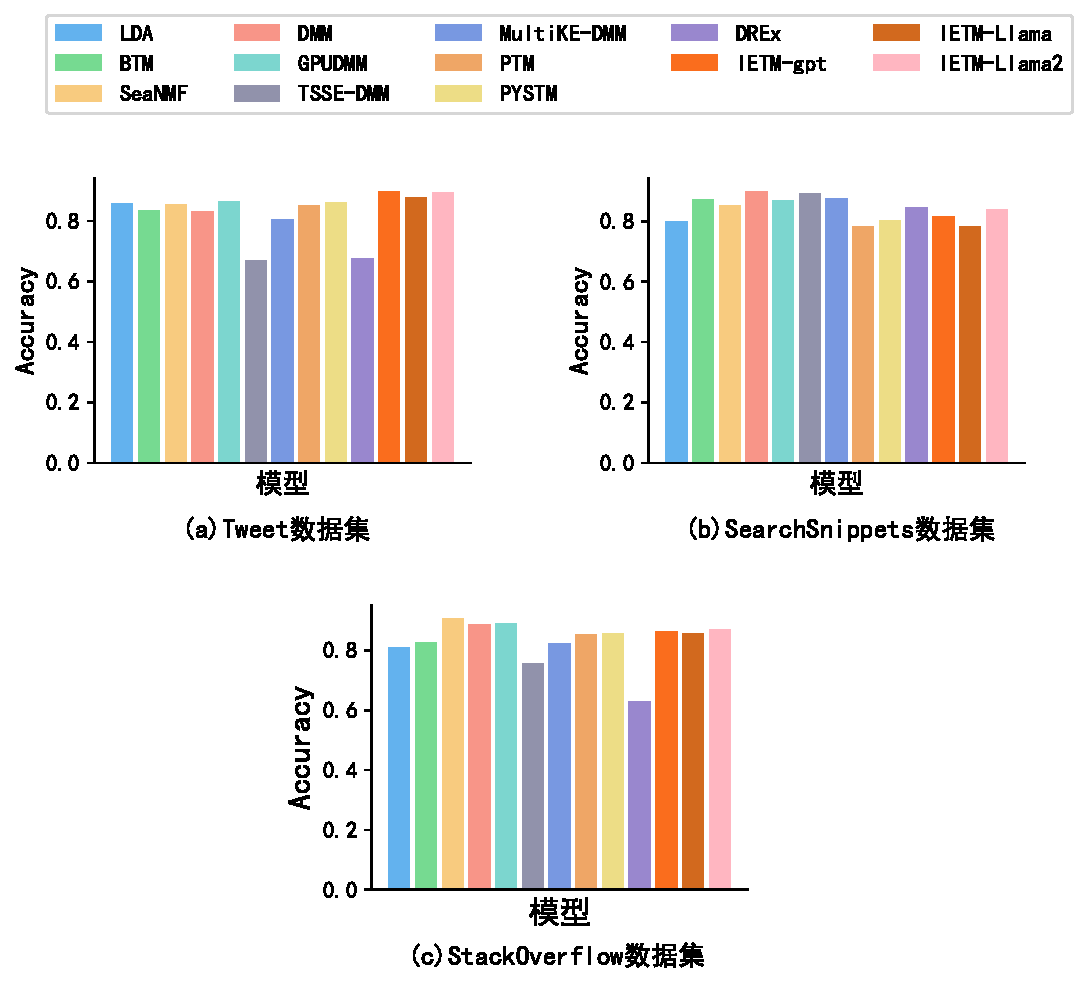
\includegraphics[width=0.85\textwidth]{chap3/Accuracy Chart.pdf}
    \caption{三个数据集的分类准确率结果图}
    \label{AccuracyChart}
\end{figure}

使用线性核支持向量机(SVM),实验在三个数据集上进行了5折交叉验证并记录平均准确率得分。具体来说,使用不同模型学习到的主题分布作为特征,并训练SVM分类器来预测每个短文本的类别。图\ref{AccuracyChart}显示,我们提出的TPTM在Tweet和StackOverflow数据集中的表现高于平均水平。然而,在SearchSnippets数据集中,TPTM无法与基线模型相比达到竞争性能。其表现不佳的一个可能原因是SearchSnippets并非严格意义上的短文本.对于Instructed-Expansion而言,这可能会导致LLMs引入不相关的语义信息。鉴于SearchSnippets数据集中只有8个类别,另一个原因可能是基于DMM的模型中使用的假设,即一个文档只关注一个主题,这对于分类任务来说更为合适。此外,可以观察到没有模型在所有数据集中都具有绝对优势。类似的结果可以在\cite{STTM}中找到。总之,我们模型学习到的主题分布具有辨别力,因此可以用于短文本分类的下游任务。

\subsection{消融实验}
如果只考虑TPTM的第一阶段,TPTM将退化为标准的LDA模型,这意味着使用LDA模型直接建模扩展后的伪文档。在本节中,我们主要讨论,与单纯使用伪文档进行LDA建模相比,通过TPTM联合建模原始文档和伪文档的有效性。本节对IE-GPT、IE-llama和IE-llama2获得的伪文档语料库使用LDA进行建模,分别命名为LDA-GPT、LDA-llama和LDA-llama2,并设定$\alpha=1.0$ 和 $\beta=0.01$。在$K=50$的条件下的结果呈现在表\ref{TableModelValidityTweet}中,其中最佳值以粗体显示。对于所有指标,本节进行了$t$检验,以显示TPTM和LDA在结果平均值上的性能差异是否具有统计显著性。如果从$t$检验中得到的$P$值低于0.05,可以认为成对性能差异是显著的。TPTM-GPT在TU得分方面表现出比LDA-GPT统计上更好的表现,而在NPMI方面的下降不显著。对于TPTM-llama和TPTM-llama2,结果也是类似的。这表明,我们提出的TPTM模型在综合主题质量方面比仅使用LDA建模伪文档更优。

\begin{table}
\centering
\caption{三个数据集在LDA和TPTM下的主题质量}
\label{TableModelValidityTweet}
\adjustbox{width=0.9\textwidth}{
\begin{tabular}{lccc|ccc|ccc}
\toprule
\multicolumn{1}{c}{\multirow{2}{*}{模型}} & \multicolumn{3}{c|}{Tweet} & \multicolumn{3}{c|}{SearchSnippets} & \multicolumn{3}{c}{StackOverflow} \\
\multicolumn{1}{c}{} & NPMI & TU & TQ & NPMI & TU & TQ & NPMI & TU & TQ \\ \midrule
LDA & 0.187 & 0.872 & \multicolumn{1}{c|}{0.163} & 0.234 & 0.799 & \multicolumn{1}{c|}{0.187} & 0.212 & 0.592 & 0.126 \\
LDA-GPT & 0.227 & 0.785$\downarrow$ & \multicolumn{1}{c|}{0.178} & 0.258 & 0.816$\downarrow$ & \multicolumn{1}{c|}{0.211$\downarrow$} & \textbf{0.242} & 0.680$\downarrow$ & 0.165$\downarrow$ \\
LDA-llama & 0.219 & 0.877$\downarrow$ & \multicolumn{1}{c|}{0.192} & 0.249 & 0.954 & \multicolumn{1}{c|}{\textbf{0.238}} & 0.228 & 0.874$\downarrow$ & 0.199 \\
LDA-llama2 & \textbf{0.230} & 0.858$\downarrow$ & \multicolumn{1}{c|}{0.197$\downarrow$} & \textbf{0.266} & 0.816$\downarrow$ & \multicolumn{1}{c|}{0.217$\downarrow$} & 0.240 & 0.743$\downarrow$ & 0.178$\downarrow$ \\ \midrule
TPTM-GPT & 0.223 & 0.818 & \multicolumn{1}{c|}{0.182} & 0.252 & 0.889 & \multicolumn{1}{c|}{0.224} & \textbf{0.242} & 0.727 & 0.176 \\
TPTM-llama & 0.216 & \textbf{0.905} & \multicolumn{1}{c|}{0.195} & 0.246 & 0.965 & \multicolumn{1}{c|}{\textbf{0.237}} & 0.224 & \textbf{0.893} & \textbf{0.200} \\
TPTM-llama2 & \textbf{0.230} & 0.877 & \multicolumn{1}{c|}{\textbf{0.202}} & \textbf{0.265} & 0.878 & \multicolumn{1}{c|}{0.233} & 0.238 & 0.789 & 0.188
\\\bottomrule
\end{tabular}}
\end{table}

\begin{figure}[ht]
    \centering
    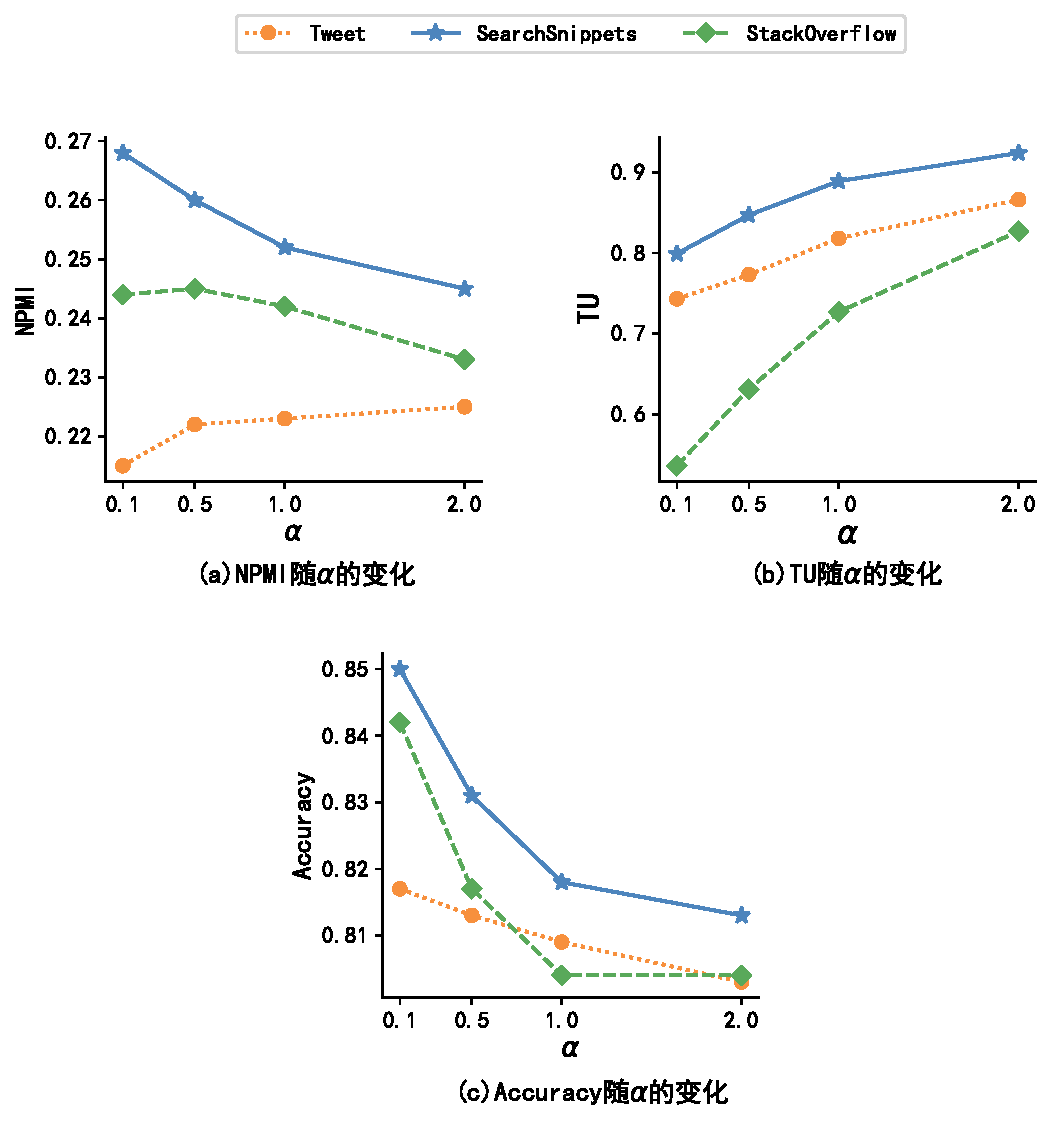
\includegraphics[width=0.8\linewidth]{chap3/resultOfAlpha.pdf}
    \caption{不同超参数值$\alpha$下的 TPTM 性能}
    \label{influenceofAlpha}
\end{figure}

\subsection{\texorpdfstring{参数$\alpha$的影响}{参数alpha的影响}}
本节在三个数据集上执行主题推断和分类任务,同时将$K$固定在50,以分析参数$\alpha$的影响。通过调整$\alpha$在${0.1, 0.5, 1, 2}$中的值,得到的结果如图\ref{influenceofAlpha}所示。总体而言,随着$\alpha$的增加,NPMI倾向于下降,而TU随着$\alpha$的增加而上升。然而,分类准确度(ACC)随着$\alpha$的增加而趋于下降。为了在主题质量和分类/聚类指标之间达到平衡,我们在上述实验中为TPTM选择了$\alpha=1.0$。

\subsection{主题展示}
本节展示了潜在主题的定性评估。以SearchSnippets数据集作为示例,因为它只包含八个类别。本节选择了与“computer”相关的主题作为示例。表\ref{Topics}展示了基线模型和TPTM挖掘出的主题示例。每个主题通过前十个词进行可视化。加粗的词表示噪音大且缺乏代表性。可以观察到这些主题聚焦于硬件、软件、操作系统、算法和网络。基线模型生成了一些具有重复词汇或主题内混淆词汇的重复主题。例如,在LDA模型得到的主题中,我们发现了一些“comedy”之类与“computer”主题无关的单词;GPU-DMM则包含“advertising”等词,并且会将细分主题网络和硬件混淆在一起;TSSE-DMM则包含许多重复且无关的单词;DREx只能挖掘出少部分与“computer”相关的词,并且也存在细分主题混淆的问题,再次验证DREx具有模糊主题之间区别的可能。相反,可以看到TPTM-llama2为对应的每个细分领域生成了一个的连贯的主题,且主题质量更高。

\section{本章小结}
在本章中,我们提出了基于提示的数据增强方法(Instructed-Expansion),以丰富短文本的词汇共现信息。此外,为了充分利用原始短文本和扩充后的伪文档,我们设计了一种新颖的方法,即基于成对文本数据的主题模型(TPTM)。在三个基准数据集上的实验表明,TPTM显著优于基线模型,有效克服了短文本的数据稀疏问题。

\begin{table}[ht]
\centering
\caption{利用各个模型从SearchSnippets数据集中挖掘的主题}
\label{Topics}
\adjustbox{width=0.9\textwidth}{
\begin{tabular}{ll}
\\\toprule
模型 & \multicolumn{1}{c}{与“computer”相关的主题示例} \\\midrule
\multirow{5}{*}{LDA} & compute parallel \textbf{comedy} \textbf{edu} \textbf{org} performance archive www http cluster \\
    & web page search home online job com dictionary definition \textbf{information} \\
    & memory intel computer chip processor apple virtual server core microsoft  \\
    & program computer language code data java tutorial web algorithm source \\
    & software system release linux download analysis project design \textbf{information} process  \\\midrule
% \multirow{5}{*}{BTM} & program java document xml instruction machine library language code web &  \\
%     & intel processor chip core amd \textbf{duo} pentium \textbf{athlon} cpu news &  \\
%     & \textbf{computer} \textbf{system} data parallel compute \textbf{edu} research information design analysis &  \\
%     & software \textbf{computer} web linux network device release security internet server &  \\
%     & memory \textbf{computer} access cache ram virtual definition disk \textbf{webopedia} \textbf{system} &  \\\midrule
\multirow{6}{*}{SeaNMF} & web search server page browser service site google website design \\
    & computer virus \textbf{memory} architecture personal \textbf{software} graphic network parallel application \\
    & program language java degree master objectoriented \textbf{tutorial} \textbf{phd} \textbf{learn} \textbf{graduate} \\
    & \textbf{software} device linux \textbf{memory} driver virtual xml disk window hardware \\
    & internet test service network connection speed bandwidth security access provider \\
    & intel processor core chip duo \textbf{pentium} amd cpu \textbf{athlon} \textbf{itanium} \\\midrule
% \multirow{5}{*}{DMM} & data algorithm \textbf{disney} system structure walt analysis consumption \textbf{consumer} design &  \\
%     & web release \textbf{software} machine instruction access \textbf{beta} wireless linux \textbf{instant} &  \\
%     & program computer \textbf{software} \textbf{wikipedia} linux driver language device web system &  \\
%     & internet network computer security bandwidth service virus test connection speed &  \\
%     & intel chip processor computer core amd cpu pentium news athlon &  \\\midrule
\multirow{5}{*}{GPUDMM} & \textbf{system} data structure xml algorithm document library respiratory analysis information \\
    & internet service share bandwidth test video connection speed \textbf{photo} \textbf{advertising} \\
    & intel memory processor chip computer amd cpu cache core virtual \\
    & computer device linux network security apple driver unix \textbf{system} virus \\
    & program web java software page computer server machine language code \\\midrule
\multirow{4}{*}{TSSE-DMM} & memory computer virtual \textbf{webopedia} cache definition \textbf{encyclopedia} \textbf{wiki} \textbf{wikipedia} web \\
    & internet network \textbf{computer} device security bandwidth access wireless \textbf{wiki} encyclopedia \\
    & programming web software java \textbf{digital} systems linux library \textbf{computer} data \\
    & intel \textbf{wiki} encyclopedia \textbf{computer} wikipedia chip software processor amd news \\\midrule
% \multirow{5}{*}{PTM}
%     & program job web java search com computer code \textbf{employment} language &  \\
%     & software management \textbf{product} system \textbf{development} tool service database engineering design &  \\
%     & computer network \textbf{digital} internet web apple \textbf{camera} \textbf{review} access wireless &  \\
%     & memory degree master virtual julia robert \textbf{graduation} cache ram \textbf{picasso} &  \\
%     & intel chip processor cpu core amd budget \textbf{pentium} \textbf{fund} athlon &  \\\midrule
\multirow{5}{*}{PYSTM} & intel chip processor amd core apple \textbf{pentium} consumption nanotechnology athlon \\
    & computer memory virtual linux operating system disk windows cache architecture \\
    & parallel computing degree \textbf{course} \textbf{thesis} master stress \textbf{phd} program \textbf{edu} \\
    & programming software java code web language source descartes release developer \\
    & server machine instruction \textbf{hypotheses} client cabinet spam web virus spyware \\\midrule
\multirow{3}{*}{DREx} 
    & network access service system security mobile computer social internet personal \\
    & computer device digital cell desktop mobile hardware intel flash memory \\
    & system information process solution product resource data management tool strategy \\\midrule
\multirow{5}{*}{TPTM-llama2} & computer memory compute virtual performance intel processor parallel chip architecture \\
    & system software device design user linux code developer download tool \\
    & data process model method analysis tool approach structure application algorithm \\
    & internet share network access user platform medium communication connect message \\
    & home web website page welcome server visit client homepage http www \\\bottomrule
\end{tabular}
}
\end{table}


\chapter{短文本主题模型的模型增强方法研究}\label{chap:sparentm}
\section{引言}
上一章提出了一种利用大规模语言模型的短文本扩充方法Instructed-Expansion,以及一种基于成对文本数据的主题模型TPTM。利用可以进行文本生成的LLMs,通过指令提示将每个短文本扩充为伪长文档,从而将LLMs的知识迁移到主题建模中。此外TPTM同时对短文本数据集和伪长文本数据集进行主题挖掘,假设短文本中的主题是从其对应伪文档中的主题中抽取的,以减轻文本生成过程中引入额外的主题信息对结果的影响。主题建模中潜在分布的参数估计是通过吉布斯采样来训练的。然而,我们也可以看到这种推理方式不够灵活,涉及大量的统计符号和公式推导,且对于大型语料库而言计算代价高昂。

近年来,深度学习的发展促使人们探索变分自编码器(VAE)\cite{VAE}来简化主题模型的推理过程 \cite{NVDM,AVITM},这一类利用神经网络搭建主题模型的方法称为神经主题模型\cite{NTMsurvey}(Neural Topic Models)。值得注意的是,使用狄利克雷分布是LDA模型成功让分布考虑平滑性和稀疏性的关键之一\cite{ZhaoPHJ}。狄利克雷变分自编码器模型(DVAE)\cite{DVAE}已成功地将狄利克雷先验约束施加于VAE网络中的表示层。然而,由于学习到的文档分布的稀疏性,VAE-LDA模型中狄利克雷先验的使用会对其挖掘出的潜在主题的质量造成影响\cite{overallQuality}。设置一个较小的狄利克雷先验值可以生成更稀疏的文档-主题分布,但这会迫使VAE将某些文档中存在的词汇分配一个几乎为零的概率,从而削弱其捕捉整个语义结构的能力\cite{DVAE,AVITM}。从而导致挖掘出的主题质量不佳的问题。因此,对文本稀疏结构的建模需要超越VAE-LDA模型中的狄利克雷先验的额外机制。上一章我们讨论了如何利用大规模语言模型增强短文本中的词共现信息。本章则聚焦于如何从模型增强的角度出发,构建一个增强稀疏表达的主题模型。

现有的工作往往修改了VAE-LDA模型中的网络架构以应对这一问题。例如批量归一化(Batch Normalization)和Dropout层被用来防止网络在训练过程中过分关注稀疏性\cite{Pachinko}。另一种方法是DVAE.Sp模型\cite{DVAE},它采用sigmoid激活函数来选择与每个文档相关的主题,旨在狄利克雷分布中解耦稀疏性和平滑性。然而,这些修改只影响训练过程,并没有将主题选择纳入主题模型的生成过程中。鉴于VAE-LDA模型中狄利克雷先验的局限性,将稀疏性考虑整合到LDA的生成过程中可能更为合适。

因此,本章在VAE-LDA框架中提出了一种新的稀疏增强的非均场主题模型(Sparsity Reinforced and Non-Mean-Field Topic Model,SpareNTM),包括两种创新的方法。首先,我们考虑一种除狄利克雷先验外的,辅助先验知识来进行稀疏性建模。在自编码框架中,一种可能的方式是使用Beta分布,如CRNTM模型\cite{CRNTM}所采用的先验,但这不能产生真正稀疏的表示。另一种方式是如TONOLINI和FALLAH等人\cite{VSC,VSCT,EVO_bi}在VAE中采用的“Spike and Slab”\cite{spike&slab}先验。但这些研究使用稀疏先验应用于图像生成领域。我们将这一想法纳入VAE-LDA模型中。因此,我们提出的SpareNTM使用二元潜变量来建模文档-主题分布中的稀疏性,即将伯努利先验引入到LDA的生成过程中。具体来说,SpareNTM为每个文档构建了一个使用伯努利变量的\textit{主题选择器},用以过滤掉不相关的主题。这样,每个文档的狄利克雷先验将被限制在所选主题的范围内。通过这种方式,我们的SpareNTM模型不仅维持了主题模型的解释性,还提高了其在处理文档集时的性能,尤其是在稀疏性较高的场景中。这种方法的关键优势在于它将稀疏性直接整合到模型的生成过程中,而不仅仅是作为训练过程中的一个调节因素。此外,通过引入二元潜变量,SpareNTM能够更有效地区分相关和不相关的主题,从而生成更加精确和一致的文档-主题分布。

其次,为了进行SpareNTM的推断步骤,我们设计了一个新颖的VAE网络,该网络采用非均场近似来估计真实后验。据我们所知,SpareNTM是首批使用非均场推理的神经主题模型之一。以往的神经主题模型\cite{CRNTM,TopicRNN,VRTM,SGTM}在引入VAE-LDA的辅助潜变量时,采用均场理论\cite{VI}对损失函数的推导过程进行简化。然而,TURNER和DREFS等人\cite{MFnegative,EVO}已经讨论了均场理论的负面影响,因为它未能解释潜变量之间的相关性。相反,我们的模型SpareNTM能够考虑到文档-主题分布与伯努利主题选择器在后验分布之间的关系。然后,我们应用“重参数化技巧”\cite{VAE}和Gumbel-Softmax估计器\cite{gumbel}来生成后验主题选择器。实验表明了我们方法在主题质量和稀疏性方面就有较大的优势。

本章的主要贡献可以总结如下:

(1)提出了一种神经主题模型,该模型使用伯努利先验对稀疏性进行建模,以获得主题质量与表示稀疏性之间的更好平衡。

(2)在VAE框架下开发了一个有效的网络结构来学习推理过程,该过程实现了后验近似中的非均场推理,以捕捉潜变量中的相关性。

(3)通过一系列实验,证明了SpareNTM在不同数据集上的主题质量和稀疏性方面优于现有模型。

\section{稀疏主题模型}
本节将描述我们提出的方法。本节首先会介绍SpareNTM的生成过程。接着提出了经过调整后的VAE主题模型,同时解释了非均场推理是如何应用的。最后详细介绍了模型对应的神经网络框架。

回顾前面章节给出的定义,给定一个包含$D$篇文本的语料库,其词汇$W$共有$V$个词汇,每篇文档$x$被处理成词袋(BOW)向量,形式为$x=[x_1,x_2,\dots,x_V]$,其中$x_i$代表第$i$个词在文档$x$中出现的次数。

% \subsection{VAE-LDA}
% 首先回顾VAE-LDA模型的框架。语料库中的每一篇文本$x$都可以被表示为在$K$个主题上,具有狄利克雷先验的一个文档-主题分布$\theta\sim Dir(\alpha)$。且主题-词分布$\beta_z$在词汇表$W$的$V$个词上对主题$z$进行建模。如果用$\beta$来表示矩阵$\beta=(\beta_1,\beta_2,\dots,\beta_K)^{T}$,文档中的词将独立同分布(i.i.d)地从分布$p(x\vert\theta;\beta)=\mbox{Multinomial}(1,\mbox{Softmax}(\theta^{T}\beta))$中抽取,被称为“product of experts”\cite{AVITM}。

% 将VAE应用于LDA模型时,模型会增加一个\textit{编码器}网络$f_{enc}$。具体来说,编码器将BOW $x$作为输入,并输出$\hat{\alpha}$,然后使用参数$\hat{\alpha}$的狄利克雷分布或其他分布$q(\theta|x;\hat{\alpha})$来近似真实的后验分布$p(\theta|x)$:
% \begin{align}
%     \hat{\alpha}:= f_{enc}(x;\Pi)\\
%     \tilde{\theta}\sim q(\theta|x;\hat{\alpha})\\
%     f_{dec}(\tilde{\theta};\beta):=\mbox{Softmax}(\tilde{\theta}^{T}\beta)
% \end{align}
% 在VAE框架下,通过最大化证据下界(ELBO)来优化编码器和解码器的参数:
% \begin{equation} 
%     \mathcal{L}(\Pi,\beta;x)=E_{q(\theta|x)}[\log p(x|\theta)]-KL(q(\theta\vert x;\hat{\alpha})\|p(\theta;\alpha))
% \end{equation}
% 在只采样一个样本的策略下\cite{VAE}, $E_{q(\theta|x)}[\log p(x|\theta)]\simeq x^{T}\log\ f_{dec}(\tilde{\theta})$.

\subsection{SpareNTM}
稀疏主题模型在传统主题模型的基础上引入稀疏假设(即每篇文档只和少量主题相关)。为了使得离散分布的采样过程能够得到有效的梯度计算以及反向传播,我们提出了稀疏增强的神经主题模型(Sparsity Reinforced Neural Topic Model, SpareNTM)。通过引入伯努利先验到文档-主题分布中,间接控制文档中的主题数量,将LDA模型与稀疏性相结合。简单来说,SpareNTM为每个主题构建一个伯努利变量,来决定该主题是否出现在当前文档中,因此每篇文档只关注少数几个主题。这样的设计可以直接在主题模型中引入稀疏性,使得每个文档的主题分布更加集中。在SpareNTM中,每个文档$d$被表示为一个包含$K$个主题的文档-主题分布$\theta\sim Dir(b_d\cdot\alpha)$,其中$b_d$是一个被称为主题选择器的向量。主题选择器$b_d=(b_{d1},…,b_{dK})$是一个长度为$K$的向量,由$K$个参数为$\lambda=(\lambda_1,\dots,\lambda_K)$的伯努利变量组成。因此,向量$b_d$鼓励文档$d$只关注一部分潜在的主题。当$b_d$的分量全为1时,SpareNTM将退化为标准的LDA模型。SpareNTM模型的生成过程如下:

\begin{enumerate}
	\item[(1)] 对于每一篇文档 $d \in \mathcal{D}$:
	\begin{enumerate}
		\item 对于主题选择器 $b_d$中的每一个分量:
		\begin{enumerate}
			\item 采样 $b_{d,k}\sim \mbox{Bernoulli}(\lambda_k)$
		\end{enumerate}
		\item 采样一个文档-主题分布 $\theta\sim \mbox{Dirichlet}(b\cdot\alpha)$
		\item 对于 $d$ 中的每个单词 $w_{n}$:
		\begin{enumerate}
			\item[] 采样一个单词实体 $w_n\sim \mbox{Multinomial}(1,\theta^{T}\beta)$
		\end{enumerate}
	\end{enumerate}
\end{enumerate}
因此,SpareNTM的编码器框架是:
\begin{align}
    \hat{\alpha},\hat{\lambda}:= f_{enc}(x;\Pi)\\
    \tilde{\theta}\sim q(\theta,b|x;\hat{\alpha},\hat{\lambda})\\
    f_{dec}(\tilde{\theta};\beta):=\mbox{Softmax}(\tilde{\theta}^{T}\beta) 
\end{align}

对于文档$d$,其联合概率密度函数为:
\begin{equation}
	\label{spLDA_joint}
	p(x,\theta,b\vert\alpha,\lambda,\beta)=p(b\vert\lambda)p(\theta\vert b;\alpha)\prod_{n=1}^{n_d} p(w_n\vert\theta;\beta)
\end{equation}
其中,假设$b$中每个分量都是独立的,有$p(b\vert\lambda)=\prod_{k=1}^{K}p(b_k\lambda_k)$。此外,可以从解码分布$p(w_n\vert\theta;\beta)=\mbox{Softmax}(\theta^T\beta)$中生成每个单词。

\subsection{目标函数}
基于上述伯努利先验的引入,我们假设一篇文章$x$对应的主题分布是$\theta$,及其伯努利主题筛选变量是$b$,其中1表示对应主题出现在该文本中,0则表示不含该主题。因此论文的目的是求得后验概率分布$p(\theta,b\vert x)$。由于此后验分布是不可求解的。在变分推断的框架下,需要推导一个变分分布$q(\theta,b|x;\hat{\alpha},\hat{\lambda})$以逼近这个后验分布。在本节中,论文为变分分布$q(\theta,b|x;\hat{\alpha},\hat{\lambda})$设计了一种基于神经网络的推断方法。传统的变分推断使用平均场理论,对潜变量之间的独立性做出强独立假设,以实现推断方法的可扩展性和易优化性\cite{VI}。以往的神经主题模型,如 TopicRNN \cite{TopicRNN}、CRNTM\cite{CRNTM}、VRTM\cite{VRTM}和SGTM\cite{SGTM},就采用平均场理论将辅助潜变量引入VAE-LDA时。然而,许多研究\cite{EVO,MFnegative}已经就无法解释潜变量之间的相关性讨论了许多关于平均场理论的负面影响。相比之下,我们定义了一个非均值场假设的变分分布Eq.(\ref{vq})来捕捉真实后验$p(\theta,b\vert x)$中$\theta$和$b$之间的相关性。
\begin{equation}
    q(\theta,b\vert x)=q(b\vert x;\hat{\lambda})q(\theta\vert x,b;\hat{\alpha})
    \label{vq}
\end{equation}
我们假设$q(b\vert x;\hat{\lambda})=\prod_{k=1}^{K}q(b_k\vert \hat{\lambda}_k)$,其中$q(b_k\vert \hat{\lambda}_k)$是具有概率$\hat{\lambda}_k$的伯努利分布。根据$p(\theta\vert b,\alpha)=\mbox{Dir}(b\cdot\alpha)$,类似地定义$q(\theta\vert x,b;\hat{\alpha})=\mbox{Dir}(b\cdot\hat{\alpha})$。在本章中,我们没有考虑$b_k$之间的依赖关系。这是因为目前我们希望模型能够捕捉到全局变量$\theta$和$b$之间的相互影响,这对于提高模型的表达能力而言更加重要。如前所述,狄利克雷分布在促进稀疏表示中也起着作用。因此,与仅依赖于二元潜变量(伯努利分布)作为先验的模型不同,$b\cdot\hat{\alpha}$有助于减轻忽略$b_k$之间依赖关系的负面影响。根据VAE-LDA模型的框架, 变分参数$\alpha$和$\hat{\lambda}=(\hat{\lambda}_1,\dots,\hat{\lambda}_K)$, 是编码器网络的输出。

通过推导变分推断背景下的证据下界(Evidence Lower Boubd,ELBO),可以优化这个非均值场的变分分布,以逼近真实的后验分布,从而提高模型在短文本主题建模中的性能和准确度。基于上述的定义,SpareNTM的证据下界(ELBO)由Eq.(\ref{myelbo})给出。这个目标可以被分解成如下形式:$\mathcal{L}=\mathcal{L}_{rec}+\mathcal{L}_\theta+\mathcal{L}_b$, where $\mathcal{L}_{rec}=E_{q(\theta,b\vert x)}\left[\log p(x\vert\theta)\right]$, $\mathcal{L}_\theta=-E_{q(\theta,b\vert x)}\left[\log\frac{q(\theta\vert x,b)}{p(\theta\vert b)}\right]$, and $\mathcal{L}_b=-E_{q(\theta,b\vert x)}\left[\log\frac{q(b\vert x)}{p(b)}\right]$。 我们的目标是最大化$\mathcal{L}$,以找到最佳的变分参数和模型参数。为了阐明ELBO所展示的内容,我们接下来详细讨论了ELBO中这三项期望的具体形式。
\begin{align}
    \label{myelbo}
    &\log(p(x,\theta,b\vert\alpha,\lambda,\beta))\geq\mathcal{L}(\Pi,\beta;x)=E_{q(\theta,b\vert x)}\left[\log p(x,\theta,b\vert \alpha,\lambda,\beta) - \log q(\theta,b\vert x)\right]\nonumber\\
	&=E_{q(\theta,b|x)}\left[\log p(x|\theta)\right]-E_{q(\theta,b|x)}\left[\log\frac{q(\theta|x,b)}{p(\theta|b)}\right]-E_{q(\theta,b|x)}\left[\log\frac{q(b|x)}{p(b)}\right]\nonumber\\
\end{align}

\textbf{(1)$\boldsymbol{\mathcal{L}_b}$}

对于$\mathcal{L}_b$,我们可以得到$\mathcal{L}_b=-\sum_{k=1}^{K}KL(q(b_k\vert x)\|p(b_k))$(推导细节见附录B.1),然后利用伯努利分布之间的KL散度计算得到解析表达式(\ref{kl2})。

\begin{equation}
    \label{kl2}
    KL(q(b_k\vert x;\hat{\lambda}_k)\|p(b_k;\lambda_k))=\hat{\lambda}_k\log\frac{\hat{\lambda}_k}{\lambda_k}+(1-\hat{\lambda}_k)\log\frac{1-\hat{\lambda}_k}{1-\lambda_k}
\end{equation}

\textbf{(2)$\boldsymbol{\mathcal{L}_\theta}$}

对于$\mathcal{L}_\theta$,我们可以得到$\mathcal{L}_\theta=-E_{q(b\vert x)}\left[KL(q(\theta\vert x,b)||p(\theta\vert b))\right]$(推导细节见附录B.2)。尽管此期望存在解析表达式,由于向量b的离散空间很大($2^K$),论文决定利用VAE中的重参数技巧\cite{VAE}处理这一表达式。通过Gumble-Softmax估计,可以从Bernoulli($\hat{\lambda}_k$)中采样得到$\tilde{b}_k,k=1,\dots,K$。因此$\mathcal{L}_{\theta}\approx-KL(q(\theta\vert x,\tilde{b})\|p(\theta\vert\tilde{b}))$,即利用狄利克雷分布之间的KL散度计算即可。

\begin{align}
	\label{kl1}
	&KL(q(\theta\vert x,\tilde{b})||p(\theta\vert \tilde{b}))=\log\Gamma(\sum_k\tilde{b}_k\cdot\hat{\alpha}_k)-\log\Gamma(\sum_k\tilde{b}_k\cdot\alpha_k)\nonumber+\sum_k\log\Gamma(\tilde{b}_k\cdot\alpha_k)\\
	&-\sum_k\log\Gamma(\tilde{b}_k\cdot\hat{\alpha}_k)+\sum_k\tilde{b}_k\cdot(\hat{\alpha}_k-\alpha_k)(\psi(\tilde{b}_k\cdot\hat{\alpha}_k)-\psi(\sum_k\tilde{b}_k\cdot\hat{\alpha}_k))
\end{align}

\textbf{(3)$\boldsymbol{\mathcal{L}_{rec}}$}

重构项是$\mathcal{L}{rec}=E_{q(\theta,b\vert x)}\left[\log p(x\vert\theta)\right]$。由于向量$b$已经在$\mathcal{L}_\theta$中被采样,并且变分分布是$q(\theta,b\vert x)=q(b\vert x)q(\theta\vert x,b)$,我们采用两步来从$q(\theta,b\vert x)$中采样$\theta$。首先,我们采样$\tilde{b}$,然后采样$\tilde{\theta}\sim\mbox{Dir}(\tilde{b}\cdot\hat{\alpha})$。因此,$\mathcal{L}{rec}$项可以近似为$\mathcal{L}{rec}\approx \log p(x\vert\tilde{\theta})=x^{T}\log\ f_{dec}(\tilde{\theta})$。

在应用SGVB(随机梯度变分贝叶斯)对变分下界(\ref{myelbo})进行优化后,现在可以重新给出模型的目标函数$\tilde{\mathcal{L}}\approx\mathcal{L}$,如下所示:
\begin{equation} 
	\begin{aligned}
		&\tilde{\mathcal{L}}(\Pi,\beta;x)=x^{T}\log\ f_{dec}(\tilde{\theta})-KL(q(\theta\vert x,\tilde{b})\|p(\theta\vert \tilde{b}))-\sum^K_{k=1}KL(q(b_k)\|p(b_k))\\
	\end{aligned}
	\label{elbo_approx}
\end{equation}
其中$\tilde{b}_k\sim\mbox{Bernoulli}(\hat{\lambda}_k)$,$k=1,2,\dots K$,且$\tilde{\theta}\sim\mbox{Dir}(\tilde{b}\cdot\hat{\alpha})$。 对于这个目标函数,我们可以明显地看出其与自编码器的联系。模型的编码器网络将文档词袋$x$映射到变分参数$\hat{\alpha}$和$\hat{\lambda}$,然后从相关分布中采样$\tilde{b}$和$\tilde{\theta}$。随后,解码器网络将$\tilde{\theta}$作为函数$\log p(x\vert\tilde{\theta})$的输入,该函数等于观测$x$的概率密度。解码器网络的目标是生成能够最大程度地重建原始观察值x的输出。网络的具体细节将在下一节中描述。

\subsection{网络框架}

完成了目标函数的推导之后,我们为其设计相应的变分自编码器网络框架。其中一个挑战是如何在VAE中实现对离散伯努利变量的采样。为了解决这个问题,我们采用类别自编码器的思想,并利用Gumbel-Softmax估计方法,以实现对伯努利变量的采样,并能够进行梯度反传优化。如图\ref{framework}所示,输入的文本$x$通过Relu激活函数以及dropout层进行线性变换。然后,上述变换的结果经过分支\ding{172},通过线性变换和批量归一化得到变分参数$\hat{\alpha}$。由于Dirichlet的参数不能为非正数,所以我们采用Softplus函数进行变换。分支\ding{173}进入主题选择模块,再次利用线性变换和批量归一化来得到$u_1$和$u_2$,分别代表主题是否被选中的比例。所以变分参数$\hat{\lambda}$(主题被选中的后验概率)是基于$u_1$和$u_2$的Softmax函数来计算的。现在可以用Gumbel-Softmax估计法从Bernoulli($\hat{\lambda}$)中对主题选择器$\tilde{b}$进行采样。对于主题第$k$个主题,定义$(\pi_{k1},\pi_{k2})=(\hat{\lambda}_k,1-\hat{\lambda}_k)$,有

\begin{equation}
	\tilde{b}_k=\frac{\exp{((\log(\pi_{k1})+g_1)/\tau})}{\sum_{i=1}^2\exp{((\log(\pi_{ki})+g_i)/\tau})}
\end{equation}
其中$g_1,g_2$是从Gumbel(0, 1)分布\footnote{Gumbel(0, 1)分布可以通过逆变换采样来抽样,方法是抽取$u\sim\mbox{Uniform(0, 1)}$,然后计算$g=-\log(-\log(u))$。}中独立同分布(i.i.d)抽样得到的,且$\tau$在实验中被设定为1。在生成主题选择器$\tilde{b}=(\tilde{b}_1,\dots,\tilde{b}_K)$之后,我们使用拒绝采样以及Gamma分布的增强采样方法\cite{DVAE,RSVI},采样稀疏的$\tilde{\theta}\sim\mbox{Dir}(\tilde{b}\cdot\hat{\alpha})$。

\begin{figure}[ht]
    \centering
    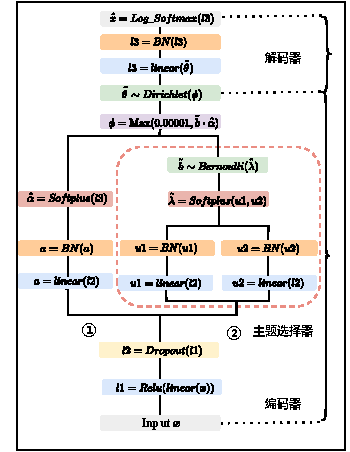
\includegraphics[trim=0cm 0.1cm 0cm 0.1cm, clip=false, width=0.65\textwidth]{chap4/network.pdf}
    \caption{SpareNTM的网络架构图} \label{framework}
\end{figure}


\section{实验设置}
\subsection{数据集}
模型的性能评估将在上一章介绍的三个短文本数据集上进行,同时增加两个常规文本对模型的鲁棒性进行评估,分别是20NewsGroups(20NG)和Wikitext-103(Wiki)\cite{wiki}。具体详情如下:
\begin{itemize}
\item \textbf{20NG} 包含大约18,000篇新闻文章,分为20个不同类别。
\item \textbf{Wiki} 是WikiText数据集的一个版本,包括来自Wikipedia的大约28,500篇文章。
\end{itemize}

对数据集进行同上一章对文本进行预处理的操作,移除了停用词以及长度等于1或出现频次少于100的单词。这两个数据集的基础信息在表\ref{corpus}中总结,其中$N$ 表示每个数据集中的文档数量,$L$ 显示每个文档的平均长度,$V$ 表示词汇表的大小。

\begin{table}
	\centering
	\caption{常规文本数据集的基本信息} \label{corpus}
	\adjustbox{width=0.35\textwidth}{
		\begin{tabular}{l|c|c|c}
			\hline
			数据集&$N$&$L$&$V$\\
			\hline
			20NG&18,846&87.5&2,000\\
                Wiki&28,532&133.4&20,000\\
			\hline
		\end{tabular}
	}
\end{table}

\subsection{对比模型}
本节将SpareNTM与LDA和以及多种不同的神经主题模型进行对比。对于常规主题模型,我们考虑了ProdLDA,DVAE。在考虑稀疏性的神经主题模型方面,我们将与DVAE.Sp,GSM,NSMDM \cite{SparseMax},SCHOLAR,和SBVAE进行比较。对于短文本数据集,我们还对比了NQTM \cite{NQTM}的效果。DVAE和SCHOLAR是最先进的神经主题模型,而NQTM在短文本中的表现优于传统主题建模。此外,我们还评估了SpareNTM-MF(使用均场假设的SpareNTM),以展示非均场推理的有效性。对比模型的详细介绍如下:

\textbf{(1)ProdLDA\cite{AVITM}:}该方法以拉普拉斯分布近似狄利克雷分布,以实现文档-主题分布在变分自编码器中的有效采样。

\textbf{(2)DVAE\cite{DVAE}:}该方法利用拒绝接受采样和伽马分布的增强采样方法,成功在变分自编码器总将狄利克雷分布作为文档-主题分布的先验分布。

\textbf{(3)DVAE.Sp\cite{DVAE}:}该方法是DVAE的稀疏化版本,其利用sigmoid激活函数构建了同我们一个目标的主题选择器变量。

\textbf{(4)GSM\cite{GSM}:}该方法利用高斯sotfmax构造( Gaussian Softmax Construction),在网络中强化隐变量的稀疏属性。

\textbf{(5)NSMDM\cite{SparseMax}:}该方法不同于GSM的稀疏构造,其采用sparsemax激活函数以进一步强化隐变量的稀疏属性。

\textbf{(6)SCHOLAR\cite{SCHOLAR}:}该方法是一种基于稀疏可加性生成模型的神经网络框架,灵活地结合了文档的元数据。

\textbf{(7)SBVAE\cite{SBVAE}:}该模型将狄利克雷过程中的Stick Breaking构造应用于变分自编码器,基于此开发了适用于主题建模的网络架构

\textbf{(8)NQTM\cite{NQTM}:}该模型基于VQ-VAE(Vector Quantised Variational AutoEncoder)构建了适用于短文本数据集的稀疏文档-主题分布。

\subsection{参数设置}
基线模型的网络结构和参数设置是根据其作者的指导构建和设置的。隐藏单元的数量设定为500,所有数据集使用200的批量大小。我们使用0.0001的学习率,并采用Adam优化器进行优化。

\section{实验结果与分析}

\subsection{与基线模型对比}
在本节中,我们将SpareNTM与基线模型进行比较。狄利克雷先验的值设置为0.02。对于SBVAE,stick-breaking先验和学习率分别设置为10和0.01。此外,对于20NG和Wiki,SpareNTM的伯努利先验设置为0.05,而在短文本数据集中设置为0.2。表\ref{Tweet topic quality},\ref{SearchSnippets topic quality}和\ref{StackOverflow topic quality}展示了在短文本数据集上,模型的NPMI指标、TU指标,以及整体主题质量TQ指标的结果。而表\ref{20News topic quality}和表\ref{Wiki topic quality}则展示了常规文本数据集上,模型的NPMI指标、TU指标和TQ指标的结果。对于每个模型,结果后的$\uparrow$或$\downarrow$表示根据5%显著性水平的t检验,该基准模型的表现显著优于或劣于我们提出的SpareNTM,并且最佳值以粗体标记。$K=50$和$K=100$的平均排名表示为av.rank。

\begin{table}
    \centering
    \caption{Tweet数据集在不同模型下的主题质量}
    \label{Tweet topic quality}
    \footnotesize
    \adjustbox{width=0.85\textwidth}{
    \begin{tabular}{cccc|cccc}
    \toprule
    \multirow{2}{*}{\textbf{Tweet}} & \multicolumn{3}{c}{K=25}&\multicolumn{3}{c}{K=50}&\\
    \cmidrule(lr){2-7}
    &NPMI&TU&\textbf{TQ}&NPMI&TU&\textbf{TQ}&av.rank\\
    \midrule
    LDA&0.187$\downarrow$ &0.872$\downarrow$ &0.163$\downarrow$ &0.184$\downarrow$ & 0.810 & 0.149$\downarrow$&3.5\\
    ProdLDA&0.181$\downarrow$&0.522$\downarrow$&0.094$\downarrow$&0.182$\downarrow$&0.415$\downarrow$&0.076$\downarrow$&10\\
    DVAE&0.179$\downarrow$&0.692$\downarrow$&0.124$\downarrow$&0.183$\downarrow$&0.426$\downarrow$&0.07$\downarrow$8&8.5\\
    DVAE.Sp&0.161$\downarrow$&0.820$\downarrow$ &0.132$\downarrow$ &0.148$\downarrow$ &0.730$\downarrow$ &0.108$\downarrow$ &6.5\\
    SBVAE&0.147$\downarrow$ &0.816$\downarrow$ &0.120$\downarrow$ &0.122$\downarrow$ &0.739$\downarrow$ &0.090$\downarrow$ &8.5\\
    GSM&0.172$\downarrow$&0.936$\downarrow$&0.161$\downarrow$&0.155$\downarrow$&0.779&0.121$\downarrow$&4.5\\
    NSMDM&0.178$\downarrow$&\textbf{0.953}&0.170$\downarrow$&0.173$\downarrow$&0.635$\downarrow$&0.110$\downarrow$&4.0\\
    SCHOLAR&0.174$\downarrow$ &0.845$\downarrow$ &0.147$\downarrow$ &0.171$\downarrow$ &0.621$\downarrow$ &0.106$\downarrow$ &6.5\\
    NQTM\cite{NQTM}&0.184$\downarrow$&\textbf{0.953}$\uparrow$&0.175$\downarrow$&0.180$\downarrow$&0.868$\uparrow$&0.156&2.0\\
    SpareNTM&\textbf{0.210} & 0.939 & \textbf{0.197} &\textbf{0.218} & 0.781 &\textbf{0.170} &1.0\\
    \bottomrule
\end{tabular}
}
\end{table}

\begin{table}
    \centering
    \caption{SearchSnippets数据集在不同模型下的主题质量}
    \label{SearchSnippets topic quality}
    \footnotesize
    \adjustbox{width=0.85\textwidth}{
    \begin{tabular}{cccc|cccc}
    \toprule
    \multirow{2}{*}{\textbf{SearchSnippets}} & \multicolumn{3}{c}{K=25}&\multicolumn{3}{c}{K=50}&\\
    \cmidrule(lr){2-7}
    &NPMI&TU&\textbf{TQ}&NPMI&TU&\textbf{TQ}&av.rank\\
    \midrule
    LDA&0.237$\downarrow$&0.804$\downarrow$&0.191$\downarrow$&0.225$\downarrow$ & 0.723$\downarrow$ & 0.163$\downarrow$&7.5\\
    ProdLDA&0.100$\downarrow$&0.709$\downarrow$&0.071$\downarrow$&0.094$\downarrow$&0.576$\downarrow$&0.054$\downarrow$&9.5\\
    DVAE&0.239$\downarrow$&0.915$\downarrow$&0.219$\downarrow$&0.246$\downarrow$&0.690$\downarrow$&0.170$\downarrow$&6.5\\
    DVAE.Sp&0.190$\downarrow$&0.868$\downarrow$&0.165$\downarrow$&0.172$\downarrow$&0.708$\downarrow$&0.122$\downarrow$&9.0\\
    SBVAE&0.230$\downarrow$&0.969$\downarrow$&0.223$\downarrow$&0.173$\downarrow$&0.702$\downarrow$&0.121$\downarrow$&7.5\\
    GSM&0.256$\downarrow$&0.968$\downarrow$&0.248$\downarrow$&0.236$\downarrow$&\textbf{0.960}&0.227$\downarrow$&2.0\\
    NSMDM&0.261$\downarrow$&0.947$\downarrow$&0.247$\downarrow$&0.214$\downarrow$&0.887$\downarrow$&0.190$\downarrow$&4.0\\
    SCHOLAR&0.253$\downarrow$&0.975$\downarrow$&0.247$\downarrow$&0.239$\downarrow$&0.863$\downarrow$&0.206$\downarrow$&3.5\\
    NQTM&0.245$\downarrow$&0.992&0.243$\downarrow$&0.238$\downarrow$&0.944&0.225$\downarrow$&4.0\\
    SpareNTM&\textbf{0.287} & \textbf{1.0} & \textbf{0.287} & \textbf{0.261} & 0.952 & \textbf{0.248}&1.0\\
    \bottomrule
\end{tabular}
}
\end{table}

\begin{table}
    \centering
    \caption{StackOverflow数据集在不同模型下的主题质量}
    \label{StackOverflow topic quality}
    \footnotesize
    \adjustbox{width=0.85\textwidth}{
    \begin{tabular}{cccc|cccc}
    \toprule
    \multirow{2}{*}{\textbf{StackOverflow}} & \multicolumn{3}{c}{K=25}&\multicolumn{3}{c}{K=50}&\\
    \cmidrule(lr){2-7}
    &NPMI&TU&\textbf{TQ}&NPMI&TU&\textbf{TQ}&av.rank\\
    \midrule
    LDA&\textbf{0.212}$\uparrow$ &0.592$\downarrow$ &0.126$\downarrow$ &\textbf{0.200} & 0.605$\downarrow$ & 0.121$\downarrow$&5.5\\
    ProdLDA&0.100$\downarrow$ &0.709$\downarrow$ &0.071$\downarrow$ &0.094$\downarrow$ &0.576$\downarrow$ &0.054$\downarrow$ &10\\
    DVAE&0.178$\downarrow$ &0.771$\downarrow$ &0.137$\downarrow$ &0.178$\downarrow$ &0.544$\downarrow$ &0.097$\downarrow$ &6.5\\
    DVAE.Sp&0.150$\downarrow$ &0.768$\downarrow$ &0.115$\downarrow$ &0.146$\downarrow$ &0.628$\downarrow$ &0.092$\downarrow$ &8.0\\
    SBVAE&0.123$\downarrow$ &0.797$\downarrow$ &0.098$\downarrow$ &0.117$\downarrow$ &0.637$\downarrow$ &0.075$\downarrow$ &9.0\\
    GSM&0.183$\downarrow$ &0.79$\downarrow$ &0.144$\downarrow$ &0.172$\downarrow$ &0.656$\downarrow$ &0.113$\downarrow$ &5.0\\
    NSMDM&0.182$\downarrow$ &\textbf{0.968}$\uparrow$ &0.176$\downarrow$ &0.170$\downarrow$ &\textbf{0.845}$\uparrow$ &0.144 &2.5\\
    SCHOLAR& 0.157$\downarrow$& 0.949&0.149$\downarrow$ & 0.14$\downarrow$& 0.732$\downarrow$&0.102$\downarrow$ &5.0\\
    NQTM&0.172$\downarrow$ & 0.957&0.164$\downarrow$ &0.176$\downarrow$ &0.844$\uparrow$ &{0.149} &2.0\\
    SpareNTM &0.203 & 0.943 & \textbf{0.191} & 0.190 & 0.785 & \textbf{0.149} &1.0\\
    \bottomrule
\end{tabular}
}
\end{table}

\textbf{(1)短文本数据集} 

从表\ref{Tweet topic quality},\ref{SearchSnippets topic quality}和\ref{StackOverflow topic quality}可以看到,SpareNTM主题质量上表现最佳。这再次证明,考虑稀疏性的模型比不考虑稀疏性的模型具有更好的主题质量。并且,由于短文本的稀疏特性,大多模型的在不同主题数量$K$下的表现不同,即模型受主题数量这一参数影响较大。所有模型在$K=50$时的主题质量都有所下降。此外,ProdLDA、DVAE.Sp和SBVAE在多数情况下的表现并不如LDA主题模型,这可能是因为这些模型的先验假设(如拉普拉斯近似狄利克雷分布,狄利克雷过程等)并在神经主题模型中并不适用。而考虑稀疏性的模型往往可以更好地挖掘出短文本中的潜在主题。尽管NQTM的表现仅次于SpareNTM,其使用离散自编码器在短文本建模中也具有天然优势,但其高内存要求使其不适用于常规文本数据集。简而言之,SpareNTM引入了额外的先验来建模稀疏性,通过非均值场的推断,同时利用了上一章提出的Instructed-Expansion方法,从而产生了较大的协同效应。
\newpage
\textbf{(2)常规文本数据集} 

从表\ref{20News topic quality}和表\ref{Wiki topic quality}可以观察到,在20NG数据集上,SpareNTM和NSMDM取得了最好的主题质量,其次是SCHOLAR和LDA。尽管在K=100时,NSMDM的表现略优于SpareNTM,但在K=50时,SpareNTM具有很大优势。在较长的Wiki数据集上,SpareNTM比其他模型表现得更好。论文提出的模型可以发现更有意义和更多样化的主题。与不考虑稀疏性的模型相比,其中DVAE具有最佳主题质量,SpareNTM表现出显著更好的主题质量。这表明狄利克雷先验优于其他先验假设。同时,作为DVAE的稀疏增强版本的SpareNTM证明了狄利克雷先验不足以满足稀疏建模的要求。考虑稀疏性的模型可以实现更好的主题质量。总之,我们发现SpareNTM相较其他模型而言,具有更广泛的适用性和鲁棒性,体现了其引入了额外的先验来建模稀疏性,且通过非均值场的推断的优越性。

\begin{table}
    \centering
    \caption{20News数据集在不同模型下的主题质量}
    \label{20News topic quality}
    \footnotesize
    \adjustbox{width=0.85\textwidth}{
    \begin{tabular}{cccc|cccc}
    \toprule
    \multirow{2}{*}{\textbf{20News}}& \multicolumn{3}{c}{K=50}&\multicolumn{3}{c}{K=100}&\\
    \cmidrule(lr){2-7}
    &NPMI&TU&\textbf{TQ}&NPMI&TU&\textbf{TQ}&av.rank\\
    \midrule
    LDA \cite{LDA}&0.248&0.580$\downarrow$&0.144$\downarrow$&0.249$\uparrow$&0.494$\downarrow$&0.123&3.5\\
    ProdLDA \cite{AVITM}&0.271$\uparrow$&0.475$\downarrow$&0.129$\downarrow$&0.250$\uparrow$&0.356$\downarrow$&0.089$\downarrow$&7.0\\
    DVAE \cite{DVAE}&\textbf{0.272}$\uparrow$&0.530$\downarrow$&0.144$\downarrow$&\textbf{0.262}$\uparrow$&0.385$\downarrow$&0.101$\downarrow$&5.0\\
    DVAE.Sp \cite{DVAE}&0.225$\downarrow$&0.525$\downarrow$&0.118$\downarrow$&0.218$\downarrow$&0.359$\downarrow$&0.078$\downarrow$&8.0\\
    SBVAE \cite{SBVAE}&0.171$\downarrow$&0.524$\downarrow$&0.090$\downarrow$&0.148$\downarrow$&0.363$\downarrow$&0.054$\downarrow$&9.0\\
    GSM \cite{GSM}&0.210$\downarrow$&0.644$\downarrow$&0.135$\downarrow$&0.200$\downarrow$&0.519$\downarrow$&0.104$\downarrow$&5.0\\
    NSMDM \cite{SparseMax}&0.222$\downarrow$&\textbf{0.784}&0.174$\downarrow$&0.200$\downarrow$&\textbf{0.651}$\uparrow$&\textbf{0.130}&1.5\\
    SCHOLAR \cite{SCHOLAR}&0.258$\uparrow$&0.603$\downarrow$&0.156$\downarrow$&0.239$\uparrow$&0.424$\downarrow$&0.101$\downarrow$&4.5\\
    SpareNTM&0.244&0.763&\textbf{0.186}&0.229&0.549&0.126&1.5\\
    \bottomrule
    \end{tabular}
    }
\end{table}

\begin{table}
    \centering
    \caption{Wiki数据集在不同模型下的主题质量}
    \label{Wiki topic quality}
    \footnotesize
    \adjustbox{width=0.85\textwidth}{
    \begin{tabular}{cccc|cccc}
    \toprule
    \multirow{2}{*}{\textbf{Wiki}} & \multicolumn{3}{c}{K=50}&\multicolumn{3}{c}{K=100}&\\
    \cmidrule(lr){2-7}
    &NPMI&TU&\textbf{TQ}&NPMI&TU&\textbf{TQ}&av.rank\\
    \midrule
    LDA&0.280$\downarrow$&0.617$\downarrow$&0.173$\downarrow$&0.286$\downarrow$&0.596$\downarrow$&0.170$\downarrow$&6.0\\
    ProdLDA&0.357$\downarrow$&0.471$\downarrow$&0.168$\downarrow$&0.377$\uparrow$&0.405$\downarrow$&0.153$\downarrow$&7.0\\
    DVAE&\textbf{0.403}&0.669$\downarrow$&0.270$\downarrow$&\textbf{0.396}$\uparrow$&0.491$\downarrow$&0.194$\downarrow$&5.0\\
    DVAE.Sp&0.197$\downarrow$&0.841$\downarrow$&0.166$\downarrow$&0.168$\downarrow$&0.701$\downarrow$&0.118$\downarrow$&9.5\\
    SBVAE&0.287$\downarrow$&0.967&0.278$\downarrow$&0.224$\downarrow$&0.580$\downarrow$&0.130$\downarrow$&6.5\\
    GSM&0.300$\downarrow$&0.974&0.292$\downarrow$&0.279$\downarrow$&\textbf{0.877}$\uparrow$&0.245$\downarrow$&3.5\\
    NSMDM&0.354$\downarrow$&\textbf{0.979}&0.347$\downarrow$&0.220$\downarrow$&0.625$\downarrow$&0.138$\downarrow$&5.0\\
    SCHOLAR&0.398&0.937$\downarrow$&0.373$\downarrow$&0.366&0.691$\downarrow$&0.253$\downarrow$&2.0\\
    SpareNTM&0.401&0.973&\textbf{0.390}&0.364&0.831&\textbf{0.302}&1.0\\
    \bottomrule
    \end{tabular}
    }
\end{table}

\subsection{消融实验} 
\textbf{(1)Instructed-Expansion数据增强的有效性}

为了评估Instructed-Expansion所得到的伪长文本对SpareNTM的影响,本节在原始短文本数据集和伪长文本数据集上分别运行SpareNTM进行比较,分别记为SpareNTM-short和SpareNTM-IE。表\ref{ablation1}展示了在这两种数据集上的运行结果。对于每个模型,结果后的$\uparrow$或$\downarrow$表示根据5%显著性水平的t检验,该基准模型的表现显著优于或劣于SpareNTM-IE可以看到Instructed-Expansion数据增强对短文本建模的提升效果是显著的。此外,尽管SpareNTM在原始短文本上的效果不如SpareNTM-IE,但与表\ref{Tweet topic quality},\ref{SearchSnippets topic quality}和\ref{StackOverflow topic quality}中的模型相比,也具有一定的竞争优势。

\begin{table}[ht]
    \centering
    \caption{原始短文本数据集和伪长文本数据集在SpareNTM下的结果。}
    \label{ablation1}
    \adjustbox{width=0.95\textwidth}{
    \begin{tabular}{lccc|ccc|ccc}
    \toprule
    \multicolumn{10}{c}{K=25}\\\hline
    \multicolumn{1}{c}{\multirow{2}{*}{模型}} & \multicolumn{3}{c|}{Tweet} & \multicolumn{3}{c|}{SearchSnippets} & \multicolumn{3}{c}{StackOverflow} \\
    \multicolumn{1}{c}{} & NPMI & TU & \textbf{TQ} & NPMI & TU & \textbf{TQ} & NPMI & TU & \textbf{TQ} \\\hline
    SpareNTM-short & 0.188$\downarrow$ &0.837$\downarrow$ &0.157$\downarrow$ & 0.230$\downarrow$&0.998&0.230$\downarrow$ & 0.176$\downarrow$ &0.973$\uparrow$ &0.167$\downarrow$  \\
    SpareNTM-IE & 0.210 & 0.939 & 0.197 & 0.287 & 1.0 & 0.287 & 0.203 & 0.943 & 0.191 \\\midrule
    \multicolumn{10}{c}{K=50}\\\hline
    \multicolumn{1}{c}{\multirow{2}{*}{模型}} & \multicolumn{3}{c|}{Tweet} & \multicolumn{3}{c|}{SearchSnippets} & \multicolumn{3}{c}{StackOverflow} \\
    \multicolumn{1}{c}{} & NPMI & TU & \textbf{TQ} & NPMI & TU & \textbf{TQ} & NPMI & TU & \textbf{TQ} \\\midrule
    SpareNTM-short & 0.180$\downarrow$ & 0.767$\downarrow$ & 0.138$\downarrow$ & 0.244$\downarrow$ & 0.978$\uparrow$ & 0.239$\downarrow$ & 0.157$\downarrow$ & 0.787 & 0.123$\downarrow$  \\
    SpareNTM-IE & 0.218 & 0.781 &0.170 & 0.261 & 0.952 & 0.248 & 0.190 & 0.785 & 0.149 \\
    \bottomrule
    \end{tabular}
    }
\end{table}

\textbf{(2)稀疏性与非均场推理方法的有效性}

为了评估将稀疏性纳入生成网络,以及SpareNTM中使用的非均场推理方法的有效性,表\ref{ablation2}将SpareNTM与,DVAE和SpareNTM-Mean-Field(SpareNTM-MF)进行比较。对于每个模型,结果后的$\uparrow$或$\downarrow$表示根据5%显著性水平的t检验,该基准模型的表现显著优于或劣于SpareNTM。尽管DVAE的NPMI得分会高于SpareNTM-MF,但在TU得分方面表现不佳。因此,在所有数据集中,SpareNTM-MF的主题质量均优于DVAE,这表明引入稀疏性增强了性能。此外,SpareNTM在它们中获得了最高的主题质量,特别是在TU得分方面,这表明了本章所提出方法的优越性,归功于在SpareNTM中应用的主题选择器和非均场推断方法。

\begin{table}
    \centering
    \caption{20News、Wiki 和 SearchSnippets分别在SpareNTM和SpareNTM-MF(使用均值场推断)下的结果}
    \label{ablation2}
    \adjustbox{width=0.95\textwidth}{
    \begin{tabular}{lccc|ccc|ccc}
    \toprule
    \multicolumn{1}{c}{\multirow{2}{*}{模型}} & \multicolumn{3}{c|}{20News} & \multicolumn{3}{c|}{Wiki} & \multicolumn{3}{c}{SearchSnippets} \\
    \multicolumn{1}{c}{} & NPMI & TU & \textbf{TQ} & NPMI & TU & \textbf{TQ} & NPMI & TU & \textbf{TQ} \\\midrule
    DVAE & 0.272$\uparrow$&0.530$\downarrow$&0.144$\downarrow$ & 0.403 & 0.669$\downarrow$ & 0.270$\downarrow$ & 0.190$\downarrow$&0.868$\downarrow$&0.165$\downarrow$ \\
    SpareNTM-MF & 0.236$\downarrow$&0.684$\downarrow$&0.161$\downarrow$ & 0.379$\downarrow$&0.940$\downarrow$&0.356$\downarrow$ & 0.214$\downarrow$ & 1.000$\uparrow$ & 0.214$\downarrow$  \\
    SpareNTM & 0.244 & 0.763 & 0.186 & 0.401 & 0.973 & 0.390 & 0.244 & 0.978 & 0.239 \\
    \bottomrule
    \end{tabular}
    }
\end{table}

\subsection{TPTM与SpareNTM的对比}
本节将SpareNTM与上一章提出的TPTM模型进行了对比。表\ref{TPTM vs SpareNTM}展示了SpareNTM和TPTM,在Tweet,SearchSnippets和StackOVerflow对应的IE-llama2数据集上的结果。对于每个模型,结果后的$\uparrow$或$\downarrow$表示根据5%显著性水平的t检验,该基准模型的表现显著优于或劣于SpareNTM。可以看到,TPTM在Tweet和StackOVerflow上的表现优于SpareNTM。一个可能的原因是Tweet数据集的样本量只有2,472,在神经网络模型中面对着样本数较少的问题,因此SpareNTM很难准确估计神经网络中的大量参数。对于StackOVerflow而言,则有可能是LLMs在获得其对应伪长文本的同时,引入了额外的主题的信息,因此TPTM更适用于此类伪文档的主题挖掘。而在SearchSnippets数据集上,SpareNTM的表现要全面优于TPTM。总之,如同Qiang\cite{STTM}等人的研究证明,没有任何一个短文本主题模型能在所有的短文本数据集上达到最优。

\begin{table}[ht]
    \centering
    \caption{K=50时,TPTM与SpareNTM在三个伪长文本数据集上的结果}
    \label{TPTM vs SpareNTM}
    \adjustbox{width=0.95\textwidth}{
    \begin{tabular}{lccc|ccc|ccc}
    \toprule
    \multicolumn{1}{c}{\multirow{2}{*}{模型}} & \multicolumn{3}{c|}{Tweet} & \multicolumn{3}{c|}{SearchSnippets} & \multicolumn{3}{c}{StackOverflow} \\
    \multicolumn{1}{c}{} & NPMI & TU & \textbf{TQ} & NPMI & TU & \textbf{TQ} & NPMI & TU & \textbf{TQ} \\\midrule
    TPTM-llama2 & 0.225 & 0.871$\uparrow$ & 0.196$\uparrow$ & 0.241$\downarrow$ & 0.874$\downarrow$ & 0.211$\downarrow$ & 0.218$\uparrow$ & 0.773 & 0.169$\uparrow$\\
    SpareNTM & 0.218 & 0.781 &0.170 & 0.261 & 0.952 & 0.248 & 0.190 & 0.785 & 0.149 \\
    \bottomrule
    \end{tabular}
    }
\end{table}

\subsection{参数影响实验}
在本节,我们首先研究了伯努利先验$\lambda$的影响。我们选择在20NG数据集上运行SpareNTM,并将狄利克雷先验$\alpha$设为0.02。表\ref{selected topics}展示了在不同$\lambda$值下,在测试集数据上计算得到的平均主题数量。可以观察到,当增加$\lambda$的取值时,SpareNTM找到的平均主题数量也随之增长,并且几乎遵循二项分布$E[\mbox{B}(K,\lambda)]=\lambda\cdot K$的期望值,而DVAE.Sp只能永远固定选择$K$个主题的一半。因此,通过结合伯努利先验,SpareNTM可以灵活地强制每篇文档专注于$K$个主题的一小部分。

图\ref{Performance_Bern}展示了在不同$\lambda$值和$K=50$条件下SpareNTM的NPMI和TU得分。可以观察到NPMI在0.230到0.250的小范围内变化,这表明本章在LDA模型中考虑稀疏性以挖掘语义信息这一方法是稳定的。相比之下,当$\lambda$增大时,TU得分下降,并在$\lambda=0.05$时获得最佳值。此时每篇文档平均选择了3个主题,这个数量小于参数设置中的主题数量$K$,甚至小于20NG中实际类别的数量。这是因为每篇文档专注于少数几个主题的假设是合理的。

\begin{table}[ht]
    \centering
    \caption{在20NG上,不同$\lambda$下,SpareNTM选择的平均主题数与DVAE.Sp进行对比} 
    \label{selected topics}
    \adjustbox{width=0.65\textwidth}{
        \begin{tabular}{c|ccccc|cc|ccc}
            \toprule
            \multicolumn{1}{c}{}&\multicolumn{7}{c}{SpareNTM}&\multicolumn{3}{c}{DVAE.Sp}\\
            \midrule
            K&\multicolumn{5}{c}{50}&100&200&50&100&200\\
            \midrule
            $\lambda$&0.2&0.4&0.5&0.6&0.8&0.1&0.1&-&-&-\\
            \midrule
            Avg.num&10&21&27&31&41&11&20&25&46&102\\
            \bottomrule
        \end{tabular}
    }
\end{table}

\begin{figure}
    \centering
        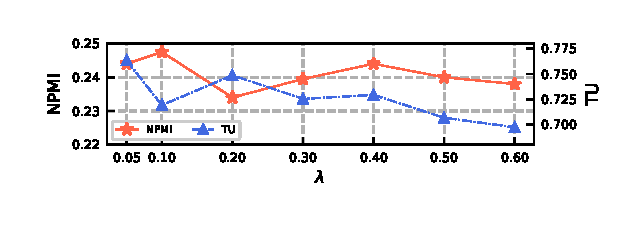
\includegraphics[trim=0.3cm 0.4cm 0.25cm 0.3cm, clip=true, width=0.8\textwidth]{chap4/Bernoulli.eps}
        \caption{在20NG数据集上,K=50时,SpareNTM在不同Bernoulli先验$\lambda$值下的NPMI和TU} \label{Performance_Bern}
\end{figure}


\begin{figure}
    \centering
        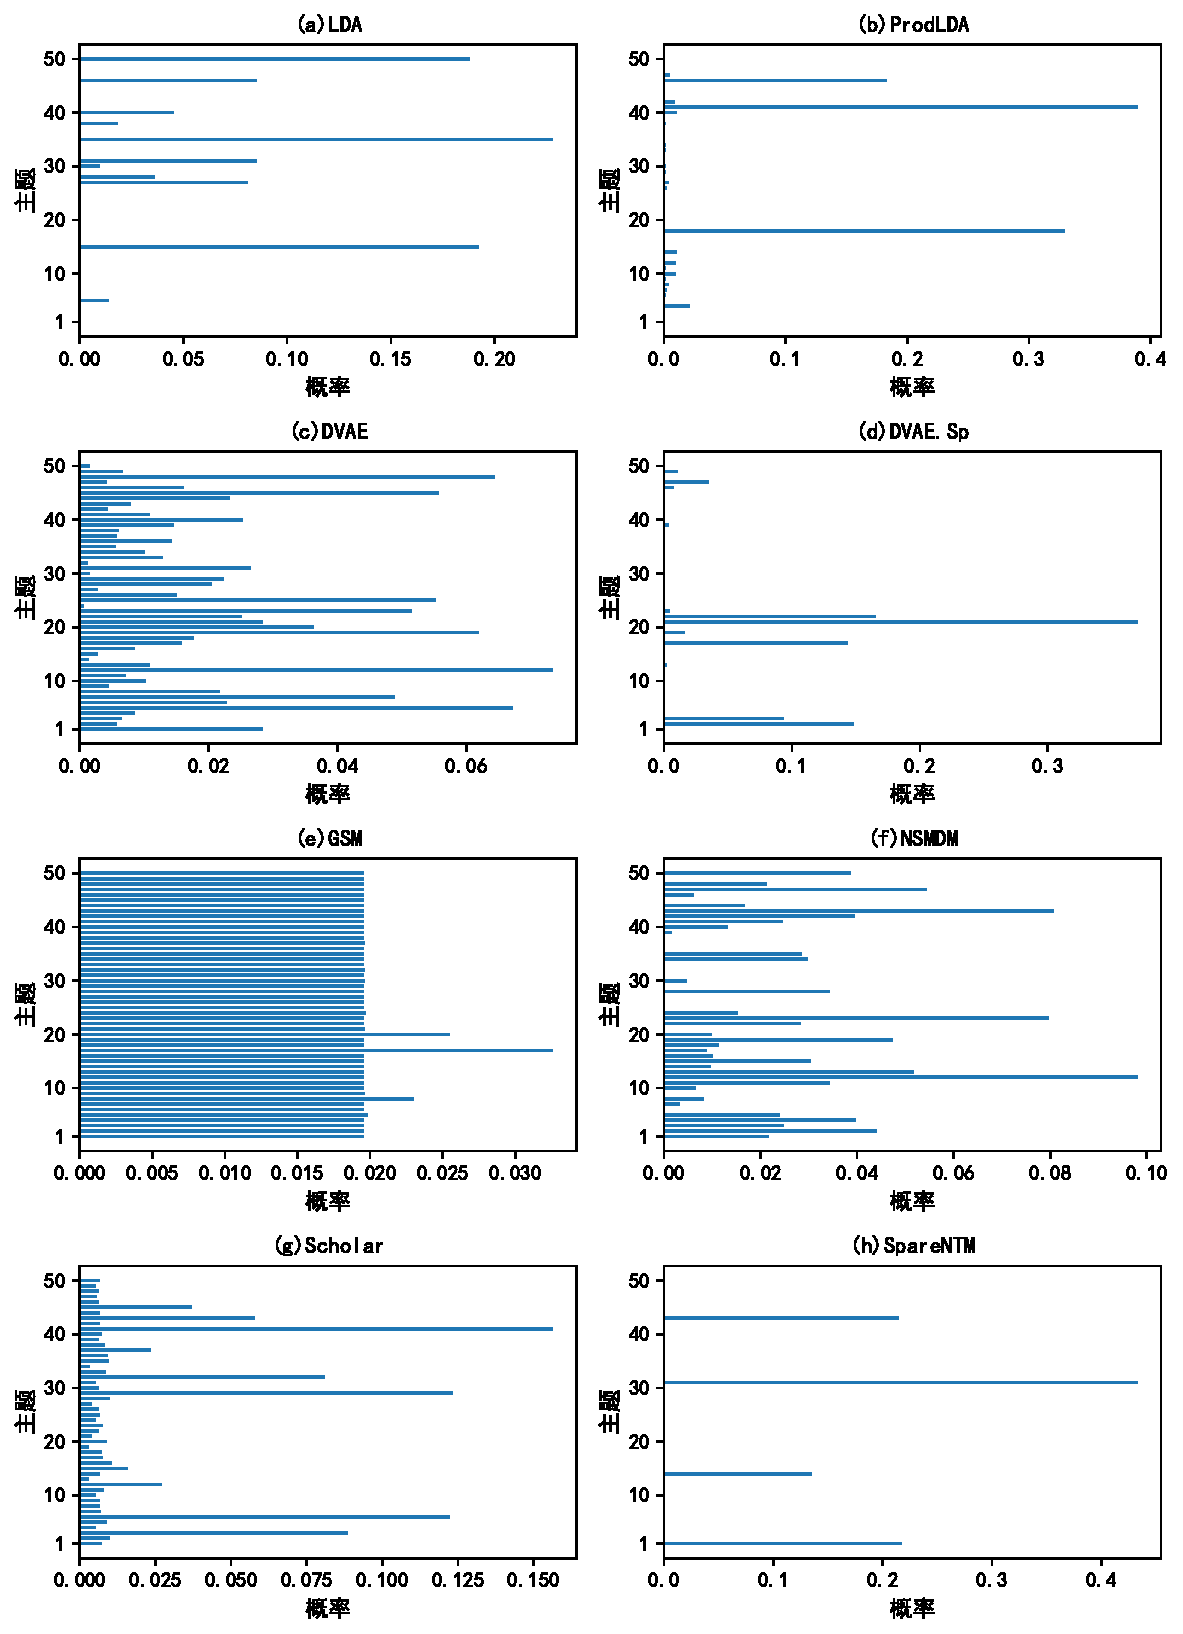
\includegraphics[trim=0.4cm 0.4cm 0.3cm 0.3cm, clip=false, width=\textwidth]{chap4/document_topic.pdf}
        \caption{当K=50时,20NG数据集中某个随机文本的文档-主题表示。以子图(h)为例,反应出该文本在只关注50个主题中的4个主题,以及在这4个主题上的概率大小。} \label{document_topic_figure}
\end{figure}
\subsection{文档-主题分布示例}
\textbf{(1)文档-主题表示示例}

本节从20NG数据集中随机选择了一篇与宗教相关的文档,并在K=50的情况下分析了不同模型生成的文档-主题表示。图\ref{document_topic_figure}中每个子图的y轴代表主题$T=[1,2,\dots,50]$,而x轴对应于主题概率。图\ref{document_topic_figure}清楚地展示了SpareNTM生成了更清晰的文档表示,这归功于其能够捕捉到每篇文档中更精确的语义信息。虽然一些基线模型也可以产生稀疏的主题分布,但我们提出的模型在稀疏的主题分布下实现了更好的主题质量。

\textbf{(2)主题示例评估} 

为了定性地展示SpareNTM生成的高质量主题,表\ref{topic examples}展示了在20NG数据集中与宗教相关的主题词,这些词是由LDA、DVAE、NSMDM、SCHOLAR和SpareNTM生成的。此外,表\ref{topic examples}将图\ref{document_topic_figure}中每个主题分布对应的两个概率最高的主题加粗显示。其他模型倾向于生成重复的主题,其中包含重复的单词。LDA和NSMDM则将不相关的主题分配给文档。相比之下,SpareNTM生成了与相关主题一致且多样化的主题。

\begin{table}[ht]
	\centering
	\caption{不同模型生成的与宗教相关的主题}
	\label{topic examples}
	\footnotesize
	\adjustbox{width=0.65\textwidth}{
		\begin{tabular}{ll}
			\toprule
            模型&\multicolumn{1}{c}{与宗教相关的主题}\\
            \midrule
            LDA&\makecell{\textbf{god believe truth one evidence}\\god jesus christian church christ\\\textbf{writes system morality keith organization}}\\
            \midrule
            DVAE&\makecell{\textbf{god Christians gods faith bible}\\jesus god bible christ faith\\heaven christ jesus sin lord\\\textbf{god Christians bible christ sin}\\morality objective evidence moral definition}\\
            \midrule
            NSMDM&\makecell{\textbf{christians biblical holy jesus sin}\\god gods faith atheist heaven\\morality objective absolute values mac\\\textbf{constitution government catholic amendment moral}}\\
            \midrule
            SCHOLAR&\makecell{god belief faith existence evidence\\god bible jesus christians christian\\christian christians god christ church\\\textbf{jesus christ church faith christians}\\\textbf{morality moral keith objective definition}}\\
            \midrule
            SpareNTM&\makecell{\textbf{jesus sin christians christ bible}\\ christ mary lord jesus heaven\\existence atheist belief islam exist\\\textbf{morality objective moral values keith}}\\
            \bottomrule
            \end{tabular}
        }
\end{table}


\section{本章小结}

本章提出了一种带有辅助伯努利变量的SpareNTM主题模型,以更好地建模文本潜在语义结构的稀疏性,并开发了一个有效的VAE网络来学习推理过程。所提出的方法可以通过识别哪些主题出现在文档中,从而发现文档-主题的稀疏性,在主题质量和泛化能力方面均优于现有方法。在多个语料库上的实验结果表明,我们的模型获得了比其他方法更高的NPMI得分和更多样化的主题。在未来的工作中,计划在在SpareNTM中考虑伯努利潜变量的相互影响时的影响。

\chapter{总结与展望}
短文本是一种非常常见的文本类型,特别是随着互联网的发展,网络上出现了大量短文本数据集,比如微博、新闻标题、商品或图片的描述、评论、问答网站的问题等等。和常规文本不同,这些短文本的长度非常有限。要挖掘这些短文本中的信息,最常用的一类方法就是主题模型。主题模型首先构造了一个隐变量:主题,并通过文本采样生成主题,再由主题采样生成词语。主题本身就成为对文本内容的归纳总结,主题和词语的关系,也让主题成为一个语义概念,人们就可以通过主题来理解文本内容。只是,传统的主题模型只适用于常规长度的文本,对于短文本集,并不能取得很好的效果。这是因为短文本集中词语共现信息不足,造成词语的共现矩阵是稀疏的。而主题模型需要利用共现矩阵产生主题稀疏的共现矩阵必然让算法的结果变的很差。我们在充分的调研已有的工作之后,提出了新的短文本主题模型方法,解决主题模型在短文本上效果不佳的问题。本文主要介绍了两个研究内容,说明了如何通过这两个研究,不断提高主题模型在短文本集上的效果。在本章中,首先对所做的主要研究工作进行了总结,归纳了创新点,然后对未来的工作进行了展望。

\section{主要贡献}

1、许多研究针对主题模型提出了各种策略和方法来解决短文本数据的稀疏性问题。一个常用的类策略是通过构建一个辅助的常规文本集, 用迁移学习的方式,先从常规长度的文本中得到语义信息,这种语义信息通常以词嵌入的形式迁移到短文本主题模型中。然而,在这类算法中,错误信息往往并来自于辅助文本集和短文本集的内容不匹配,从辅助文本集得到的语义信息并不能够代表短文本集的语义信息。此外,构建辅助文本集的直接方法是从短文本自身入手,对其扩充而达到数据增强的目的,从而增加文档层面的词共现信息。但现有的文本扩充方法无法保留文本原来的语义信息,即扩充之后的“伪”长文与原来的短文之间存在语义不一致的问题。

为了解决以上问题,本文提出了一种数据增强的新方法,将每个短文基于大规模语言模型扩充为一个(伪)长文本,解决了以往短文本集和伪长文本集在语义上不一致的问题。与以往大多数工作中使用传统主题模型对扩充后得到的长文本进行主题挖掘不同,本论文研究了一个将伪长文本与原始的短文联合建模的主题模型,完善了数据增强之后的主题建模方法。

2、一些主题模型针对短文本的稀疏性问题引入了额外的正则化约束项或稀疏先验分布。在传统的非深度学习框架下,这些模型的推导求解非常复杂。而这些主题模型中潜在分布的参数估计往往是通过吉布斯采样来学习的。然而,这种推理方式不够灵活,且对于大型语料库而言计算代价高昂。基于神经网络(如变分自编码器)的主题模型可以加快推理速度,但这些神经主题模型更多地针对长文本设计,缺乏文本稀疏性相关的研究。

为了解决以上问题,本论文提出研究神经稀疏主题建模方法,弥补了神经主题模型在稀疏性建模上的不足。同时,突破了自编码器变分推断中常用的均值场假设,首次利用变分自编码器实现基于非均值场推断的主题模型,提高了模型的表达能力,更好地捕捉到文本集的主题结构。

\section{未来展望}
尽管,在短文本主题挖掘领域,本文提出了一系列解决方法和新模型,在该领域中仍然还有许多待探索和解决的关键问题。未来 的研究可能有以下几个方向。

1、本文第三章的方法是将大型语言模型的知识转移到短文本主题建模中,以此来改进挖掘出的潜在主题的质量。然而,本文在基于指导的文本扩充中所使用的指令提示可能是随意和简单的,可能会导致扩充得到的伪文档质量不高。因此如何在目标数据集上对大规模语言模型进行微调以获得更适合于主题建模的伪文档是一个可能研究方向。此外,在本文中,数据增强的方法与主题建模的方法是分开的,需要探讨的是,是否有可能仅依靠大规模语言模型,比如直接使用原始短文本作为大模型的输入,来有效地完成主题建模任务,而不需要额外的数据处理或算法支持。

2、在第四章本文定义的基于非均值场假设的变分分布中,我们更关注两个全局变量“文档-主题分布”和“主题选择器”之间的相互影响,而忽略了“主题选择器”各个分量之间的依赖关系。已有研究提出了一些二元隐变量(稀疏编码)的非均值场变分神经网络。尽管这些模型只用了这一稀疏编码作为数据的隐变量,一个可以参考的方向就是利用他们的方法对“主题选择器”的依赖关系进行建模,从而进一步提高本文模型的表达能力。
%- 
\backmatter% 初始化其他部分环境,不建议注释
%-
\szubibliography% 导入参考文献
%-
\chapter[附录]{附录A\ \ xxxxxx}
\markboth{附录A\ \ xxxxxx}{}

% 导入附录
\chapter*{附录B\ \ xxxxxx}
\markboth{附录B\ \ xxxxxx}{}

%-
%- 2020年新增,添加答辩记录,建议分成三个独立的PDF文件,
%- \szuaddpdf命令包含两个参数,[]中为可选参数,用于生成目录,{}中为PDF文件名,默认在Image下
% \szuaddpdf[指导教师对研究生学位论文的学术评语]{pingyu}
% \szuaddpdf[学位论文答辩委员会决议书]{dabian1}
%-\szuaddpdf{dabian2}% 前一页生成目录即可
%-
\chapter[致谢]{致\quad{}谢}
% 导入致谢
%-
\chapter{攻读硕士学位期间的研究成果}

%- 可以直接使用引用的格式

\begin{enumerate}[label = {[\arabic*]}]
    \item \underline{Chen, J.}, Wang, R., He, J., Li, M. J. (2023, September). Encouraging Sparsity in Neural Topic Modeling with Non-Mean-Field Inference. In Joint European Conference on Machine Learning and Knowledge Discovery in Databases, ECML-PKDD (pp. 142-158). Cham: Springer Nature Switzerland. (CCF B 类会议)
    \item Li, M. J., \underline{Chen, J.}, Li, J., Wang, R., Zhang, Q.. Transferring Knowledge from Large Language Models for Short Text Topic Modeling. International Conference on Data Engineering, ICDE. (CCF A 类会议,在投)
    \item He, J., \underline{Chen, J.}, Li, M. J. (2022, November). Multi-knowledge Embeddings Enhanced Topic Modeling for Short Texts. In International Conference on Neural Information Processing (pp. 521-532). Cham: Springer International Publishing. (CCF C 类会议)
    \item Li, M. J., Wang, R., Li, J., Bao, X., He, J., \underline{Chen, J.}, He, L. (2023, November). Topic Modeling for Short Texts via Adaptive P{\'{o}}lya Urn Dirichlet Multinomial Mixture. In International Conference on Neural Information Processing (pp. 364-376). Singapore: Springer Nature Singapore. (CCF C 类会议)
\end{enumerate}

% 导入研究成果
%-
\end{document}
% %---------------------------------------------------------------------------%
